\documentclass{like}

%\selectlanguage{english}
%\selectlanguage{german}

\usepackage{amsmath}
\usepackage{pgfplotstable}
\usepackage{pgfplots}

%benötigt für code include
\usepackage{listings}
\usepackage{color}
\begin{document}



%%%%%%%%%%%%%%%%%%%%%%%%%%%%%%%%%%%%%%
%% Ab hier beginnt der Text
%%%%%%%%%%%%%%%%%%%%%%%%%%%%%%%%%%%%%%
  

%\normalsize
%Define our elements for our title page
\makeatletter

\renewcommand{\title}[1]{\gdef\@title{#1}}
\newcommand{\artderarbeit}[1]{\gdef\@artderarbeit{#1}}
\renewcommand{\author}[1]{\gdef\@author{#1}}
\newcommand\@matrikelnummer{\relax}
\newcommand{\matrikelnummer}[1]{\gdef\@matrikelnummer{#1}}
\newcommand{\professor}[1]{\gdef\@professor{#1}}
\newcommand\@studiengang{\relax}
\newcommand{\studiengang}[1]{\gdef\@studiengang{#1}}
\newcommand{\university}[1]{\gdef\@university{#1}}
\newcommand{\faulogo}[1]{\gdef\@faulogo{Abbildungen/#1}}
\newcommand{\likelogo}[1]{\gdef\@likelogo{Abbildungen/#1}}
\newcommand{\submitdate}[1]{\gdef\@submitdate{#1}}
\newcommand{\startdate}[1]{\gdef\@startdate{#1}}
\newcommand{\declaration}[1]{\gdef\@declaration{#1}}
\newcommand\@betreuerB{\relax}
\newcommand{\betreuerB}[1]{\gdef\@betreuerB{#1}}
\newcommand\@betreuerC{\relax}
\newcommand{\betreuerC}[1]{\gdef\@betreuerC{#1}}
\newcommand\@betreuerD{\relax}
\newcommand{\betreuerD}[1]{\gdef\@betreuerD{#1}}
 
%-----------------------------------------------------------------------
% Title page definition.
%-----------------------------------------------------------------------
\newcommand{\titlep}{
        \thispagestyle{empty}
        \begin{titlepage}
		\enlargethispage{4cm}
%        \null
		\vspace*{-2cm} 
        \begin{center}
{\rmfamily\large \textbf{ Friedrich-Alexander-Universität Erlangen-Nürnberg}}
\vskip 1,4cm
\begin{center}
%\includegraphics[scale=0.80, natwidth=1024, natheight=200]{\@faulogo} \hfill
\includegraphics[scale=0.80]{\@faulogo} \hfill
\vskip .8cm
{\large \bfseries Lehrstuhl für Informationstechnik\\(Schwerpunkt Kommunikationselektronik)}
\vskip 1.2cm
%\includegraphics[scale=0.40, natwidth=1024, natheight=200]{\@likelogo} \hfill
\includegraphics[scale=0.40]{\@likelogo} \hfill
\end{center}
\vskip .3cm
{\Large \@artderarbeit~mit dem Thema:\\}
\vskip 1.7cm
{\rmfamily\Large\bfseries\expandafter{\@title}}
        \end{center}
\vskip 1.5cm
		
\begin{table}[h!]
	\flushleft
%\setlength{\tabcolsep}{10pt}
	\large
\renewcommand{\arraystretch}{1,1}
	\begin{tabular}{p{4cm}l}
Bearbeiter     & {\rmfamily\large\expandafter{\@author}}\tabularnewline[.6ex]
\ifthenelse{\equal{\@matrikelnummer}{\relax}}{} {Matrikelnr. & \textrm{\@matrikelnummer}\tabularnewline[.6ex]}
\ifthenelse{\equal{\@studiengang}{\relax}}{}    {Studiengang & \textrm{\@studiengang}\tabularnewline[.6ex]}
Betreuer  & {\rmfamily\large\expandafter{\@professor}}\tabularnewline[.6ex]
                & \ifthenelse{\equal{\@betreuerB}{\relax}}{\vspace*{-0.6cm}}{\rmfamily\large{\@betreuerB}} \tabularnewline[.6ex]
                & \ifthenelse{\equal{\@betreuerC}{\relax}}{\vspace*{-0.9cm}}{\rmfamily\large{\@betreuerC}}  \tabularnewline[.6ex]
                & \ifthenelse{\equal{\@betreuerD}{\relax}}{\vspace*{-0.7cm}}{\rmfamily\large{\@betreuerD}} \tabularnewline[.6ex] Beginn         & {\rmfamily\large\expandafter{\@startdate}}\tabularnewline[.6ex]
Ende           & {\rmfamily\large\expandafter{\@submitdate}}            
	\end{tabular}
\end{table}
	        \vskip1cm
        \end{titlepage}
        \newpage}
        \makeatother
        
 


%-----------------------------------------------------------------------
% redefined \maketite
%-----------------------------------------------------------------------
\renewcommand{\maketitle}{%
                \titlep
	     }
%-----------------------------------------------------------------------
%  hier die eigenen Daten eintragen
%----------------------------------------------------------------------
    
\title{Modellfehler in optimierungsbasierter kombinierter Planung und Regelung für Rennwagen} % Mussfeld
\artderarbeit{Masterarbeit}         % Mussfeld
\author{Weller Sebastian}               % Mussfeld
\studiengang{Informations und Kommunikationstechnik}        % if Feld
\matrikelnummer{21777345}         % if Feld
\faulogo{fau.png}                   % Mussfeld
\likelogo{like.png}                 % Mussfeld
\professor{Prof. Dr.-Ing. Jörn Thielecke}       % Mussfeld
\betreuerB{Henrik Bey, M.\,Sc.}           % if Feld
%\betreuerC{Florian Particke, M.\,Sc.}              % if Feld
%\betreuerD{Betreuer D}             % if Feld  u.U. auskommentieren 
\startdate{08. Januar 2018}         % Mussfeld
\submitdate{09. Juli 2018}        % Mussfeld

% \maketitle

\maketitle
%BESTÄTIGUNG

\chapter*{Bestätigung}


\textbf{Erklärung:}\\

Ich versichere, dass ich die Arbeit ohne fremde Hilfe und ohne Benutzung anderer als der angegebenen Quellen angefertigt habe und, dass die Arbeit in gleicher oder ähnlicher Form noch keiner anderen Prüfungsbehörde vorgelegen hat und von dieser als Teil einer Prüfungsleistung angenommen wurde. Alle Ausführungen, die wörtlich oder sinngemäß übernommen wurden, sind als solche gekennzeichnet.
\vskip 2.5 cm
Erlangen, den (hier Datum eintragen)%{\rmfamily{\@submitdate}}
 \underline{\hspace{7cm} }
\vskip 1.5 cm

%DANKSAGUNG
%\pagestyle{scrheadings}
\chapter*{Danksagung}
%\headmark%chapter = Titel
%\section*{}
Ich möchte mich bei meinen Betreuern und meiner Familie bedanken.....

 %Optional
%Thema und Aufgabenstellung
 
%\pagestyle{scrheadings}

\chapter*{Thema und Aufgabenstellung}
\markboth{Thema und Aufgabenstellung}{Thema und Aufgabenstellung}
\textbf{Thema:}\par\smallskip

 Modellfehler in optimierungsbasierter kombinierter Planung und Regelung für Rennwagen

\textbf{Aufgabenstellung:}\par\smallskip
\par\smallskip  
Die Automatisierung des Fahrens schließt sowohl die Planung als auch die Regelung des Fahrzeugs mit ein. Häufig werden beide Bestandteile hierarchisch voneinander getrennt. Dies ist sinnvoll, solange das kontrollierte Fahrzeug sicher innerhalb der Aktuator\-li\-mi\-tie\-rungen betrieben werden soll, oder wenn die Trennung bereits durch die Problemstellung gegeben ist (Zieltrajektorie bereits vorgegeben) \cite{Williams2016AggressiveDW}.  

In anderen Fällen, z.B. wenn die gewünschte Dynamik wie in einer Rennsituation im Grenzbereich liegt, bietet sich eine kombinierte Planung und Regelung an. In diesem Beispiel würde die Kostenfunktion eine Minimierung der Rundenzeit beinhalten, während gleichzeitig die Beschränkungen des Fahrzeugs berücksichtigt werden.

Für derartige Probleme ist die modellprädiktive Regelung (MPC) bzw. eines ihrer Derivate besonders geeignet. Dabei kommt es immer zu einem sogenannten Modellfehler, der von der Komplexität und Genauigkeit des verwendeten Modells abhängt.

Das Ziel dieser Arbeit ist es, den Abfall bei der Leistung des Regelungsansatzes durch den Modellfehler zu untersuchen. Dafür soll eine Simulation verwendet werden.
Die Arbeit soll folgende Punkte beinhalten:
\begin{itemize}
\item Auswahl einer passenden Simulationsumgebung und deren Inbetriebnahme
\item Implementierung verschiedener (gegebener) Modelle für die Simulation
\item Implementierung des MPC-Ansatzes
\item Entwicklung einer einfachen Evaluationsmethode, um die Leistungsfähigkeit des Reglers zu untersuchen
\item Vergleich verschiedener Kombinationen aus Regler- und Simulationsmodellen
\end{itemize}
%Kurzzusammenfassung

\chapter*{Kurzzusammenfassung}

Mit zunehmender Rechenleistung und Erfahrung der Automobilbranche mit autonomen Fahrzeugen rückt auch das Thema der selbstfahrenden Rennautos immer mehr in den Fokus. Das ROBORACE Projekt ist hier Vorreiter mit seiner ausgefeilten Hardwareplattform und dem bereits in öffentlichen Events gezeigten Fahrleistungen. Auch die Formula Student (FS) verschließt sich nicht vor dem Trend und hat 2017 die Rubrik Driverless ins Leben gerufen. \\
Diese Masterarbeit beschreibt einen Ansatz zur Echtzeitregelung und Trajektionsplanung für ein eben solches Driverless-Racecar. Die Basis hierfür ist ein Model Predictive Control (MPC) Algorithmus. Er vereint die Regelung und Trajektionsplanung und ist sehr adaptiv bezüglich verschiedener Fahrsituationen und Ziele.
Als Ausgangssituation wird angenommen, dass das Fahrzeug bereits eine Runde auf einem unbekannten Kurs absolviert und nun eine genaue Karte des Kurses errechnet hat. 
Um das MPC nutzen zu können muss ein Fahrzeugmodell hinterlegt werden. Je genauer dieses ist, desto näher kann die Regelung an die Grenzen des realen Fahrzeuges gehen. Neben der Auslegung für das aktuellste FS-Fahrzeug des High Octane Motorsports für die Driverless Umrüstung, wird untersucht ab welchem Punkt ein kinematisches Modell nicht mehr ausreicht um das Fahrzeug sicher auf dem Rennkurs zu führen.



%\abstract 
\chapter*{Abstract}
In recent years with more and more computational power and sophisticated algorithms, autonomous cars are close to becoming a reality. An ancillary effect of this development is the emerging of driverless racecars. For this idea to become a reality, three key ingredients have to be met. A very good approximation of the location of the racecar in a virtual map, a trajectory planning algorithm and a controller that will drive the car on the computed path. In this thesis the model predictive control(MPC) algorithm is used, to combine the trajectory planning and controlling for an autonomous race car, build for the formula student driverless competition. A simulation environment will be developed to evaluate the effectiveness of the approach. One key part of this thesis is to investigate how prone to model errors the MPC-approach is and what performance can be expected for the use of a kinetic bicycle model as system description in the (MPC)-algorithm.
%%Abkürzungsverzeichnis
%\pagestyle{scrheadings}
%\chapter*{Abkürzungsverzeichnis}

\chapter*{Abkürzungsverzeichnis}
\addcontentsline{toc}{chapter}{Abkürzungsverzeichnis} %Abkürzungsverzeichnis kommt ins InhaV.





\begin{acronym}[SEPSEP] 
 \acro{Abk.}{Abkürzung}
 \acro{z.B.}{zum Beispiel}
 \acro{MPC}{Model Predictive Control}
 \acro{JIT}{just-in-time}
 \acro{SLSQP}{Sequential Least SQuarez Programming}
\end{acronym}


 (nach hinten verschoben)

\tableofcontents % erstelle hier das Inhaltsverzeichnis
\markboth{Contents}{Contents}
%\listoffigures % erstelle hier das Abbildungsverzeichnis 
%\listoftables % erstelle hier das Tabellenverzeichnis
\enlargethispage{2cm} %Bitte 2x kompilieren - sonst erscheint es nicht


\pagenumbering{arabic} %Seitennummerierung arabisch
\setcounter{page}{1}   %1. Kapitel soll mit Seitenzahl 1 beginnen
%------------------------------------------------------------------

\chapter{Einleitung}
Neben neu aufkommenden Trends in der Automobilindustrie, wie dem Elektroauto, Carsharing und dem aktuellen SUV-Boom, hat sich vor allem das autonome Auto in den letzten zwei Jahren mit dem Aufkommen von Teslas Autopilot stark in das Zentrum der Aufmerksamkeit von Firmen und Konsumenten gerückt. Das Jahr 2018 markiert dabei einen ganz besonderen Meilenstein. 
Ende des Jahres wird die Alphabet-Tochter Waymo die ersten vollautonomen Taxis in Phoenix für die Öffentlichkeit in Betrieb nehmen \cite{Waymo:1}. 
Dies ist jedoch nur möglich, da Google im gesamten Gebiet, in dem sie ihren Service anbieten werden, eine hochgenaue Umgebungskarte in die Software der Fahrzeuge integriert. Sollen die Fahrzeuge in unbekannten Umgebungen agieren, müssen sowohl die Sensorsysteme, als auch die Algorithmen noch deutlich weiterentwickelt werden, bevor autonome Autos der sogenannten Stufe 5 frei verfügbar sind. Die Unterteilung dieser Level wurde von der Bundesanstalt für Straßenwesen zur Klassifizierung von selbst fahrenden Autos erstellt \cite{BASt5L}. Die Spanne geht von Stufe 0, keinerlei Assistenz beim Fahren, bis Stufe 5, Vollautomatisierung. In dieser höchsten Stufe kann das Fahrzeug jederzeit ohne das Eingreifen des Fahrers navigieren. 
Nicht nur in den großen Automobilkonzernen wird deshalb zum Erreichen der höchsten Automatisierungsstufe geforscht. Bereits in der Schule, aber vor allem an Universitäten und Hochschulen, gibt es immer mehr Projekte, an denen die Studenten sich intensiv mit der Entwicklung autonomer Roboter und Fahrzeugplattformen beschäftigen. Ein solches Projekt ist der \ac{FS} Driverless-Wettbewerb.

\section{Formula Student Driverless}
Die Formula Student ist ein Ingenieurswettbewerb für Studenten. Er hat seine Wurzeln in den USA und wurde im Jahre 1981 das erste mal ausgetragen. Das Ziel des Wettbewerbes ist es, im Verlauf eines Jahres ein eigenes Rennauto zu konzipieren, designen, fertigen und sich schlussendlich mit anderen Teams zu messen. Dass der Wettbewerb sehr erfolgreich ist, machen nicht nur die inzwischen fast 700 Teams weltweit \cite{FsWorldRank:1} deutlich, sondern auch die Anzahl der verschiedenen Events, die überall auf der Welt im Sommer stattfinden. Seit dem Jahr 2017 gibt es neben der ursprünglichen Combustion-Klasse und der vor 10 Jahren eingeführten Electric-Klasse auch noch die Driverless-Klasse.
In dieser wird von den Teams ein Altfahrzeug mit Sensoren und Aktoren so erweitert, dass das Rennauto die Kurse autonom befahren kann.
Der Wettbewerb ist unterteilt in dynamische und statische Disziplinen. In letzteren werden verschiedene Präsentationen von den Teams ausgearbeitet. Diese beziehen sich auf die technische Realisierung, Softwaredesign, Kostenaufstellung und einen Businessplan.
Die dynamischen Disziplinen, in denen das Fahrzeug selbstständig fährt, sind:
\begin{itemize}
	\item Acceleration \\ Ein 75 Meter langer Beschleunigungsstreifen. Punkte werden nach der Zeit, nicht nach der Endgeschwindigkeit vergeben.
	\item Skidpad \\ Eine liegende 8, bei der an der Engstelle eingefahren wird und jeweils zwei rechte und zwei linke Runden gefahren werden. Die zweite Runde geht jeweils in die Zeitmessung ein. Die Abmaße sind exakt vorgegeben.
	\item Trackdrive \\ Ein bis zu 800 Meter langer Kurs mit maximal 80 Meter langen Geraden und Kurven mit einem minimalen Innenradius von neun Metern. Es werden elf Runden gefahren und die Teams erhalten im Vornherein keine Möglichkeit, Messungen am Kurs vorzunehmen.
\end{itemize}

Für die vorliegende Arbeit ist vor allem der Trackdrive von Interesse. Es wird davon ausgegangen, dass das Fahrzeug bereits die erste Runde absolviert und sich damit eine genaue Karte des Rennkurses erstellt hat. Die Messungen und Vergleiche beziehen sich damit auch immer auf einen Kurs, der so in einem \ac{FS}-Event für die Driverless-Fahrzeuge vorkommen könnte. 
In der Abbildung \ref{fig:zurichDriverless} ist das autonome Rennauto von Zürich zu sehen, wie es den Trackdrive absolviert.
\begin{figure}[hb!]
	\centering
	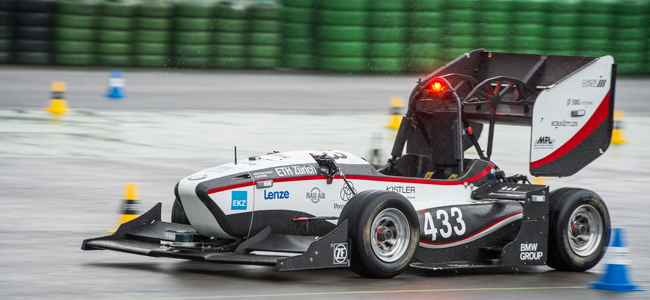
\includegraphics[width=270pt]{Abbildungen/amz-driverless-long.jpg}
	\caption{Zürichs \ac{FS}-Driverless-Fahrzeug im Jahr 2017 während des Trackdrive}
	\label{fig:zurichDriverless}
\end{figure}

\section{Problemstellung}
Im Laufe dieser Arbeit soll ein Algorithmus entwickelt werden, der die Trajektorienplanung und Regelung eines \ac{FS} Driverless Racecars berechnet. Der dafür gewählte Ansatz ist \ac{MPC}. Es handelt sich dabei um ein Verfahren, welches die Planung von Trajektorien und die Steuerung des Rennautos in einem Algorithmus vereint. Wie der Name schon sagt, wird hierfür ein Modell des zu kontrollierenden Systems benötigt, mit dem daraufhin das zukünftige Verhalten vorausberechnet werden kann. Dieses Wissen wird genutzt um mit Hilfe einer Kostenfunktion die Steuerparameter so zu variieren, dass das Rennauto eine möglichst schnelle Rundenzeit erreicht. In der Arbeit wird untersucht, wie groß die Unterschiede zwischen einem rein geometrischen Fahrzeugmodell und einem um Reifenkräfte erweiterten, für hohe Geschwindigkeiten realistischeren, Modell sind. Zudem wird evaluiert, unter welchen Einschränkungen der \ac{MPC}-Ansatz mit hinterlegtem kinematischen Modell ein dynamisches Modell im Simulator steuern kann. Das Ziel ist also eine möglichst niedrige Rundenzeit zu erreichen unter der Voraussetzung, dass das Fahrzeug immer auf dem Kurs bleibt.


\chapter{Stand der Technik}
Obwohl es zum Zeitpunkt der Arbeit noch keine öffentliche, autonome Rennserie außerhalb der Formula Student gibt, ist das Interesse an den dafür benötigten Technologien sehr groß.
Einen guten Rennfahrer zeichnet die Tatsache aus, dass er sein Fahrzeug in absoluten Grenzsituationen noch unter Kontrolle halten kann. Diese Eigenschaft ist nicht nur für autonome Rennautos wichtig, sondern ganz besonders auch für aktive Fahrassistenzsysteme. In kritischen Fahrsituationen, in denen ein ungeübter Fahrer einen Unfall nicht mehr verhindern kann, können diese Systeme noch eingreifen. Um einen guten Rennfahrer in Software nachstellen zu können, müssen drei Grundvoraussetzungen geschaffen werden:
\begin{itemize}
	\item Genaue Kenntnis der Umgebung (dem Rennkurs) und der eigenen Position
	\item Möglichst viel Wissen über das Verhalten des Fahrzeugs (Fahrzeugmodell)
	\item Kurze Reaktionszeiten (engl.: muscle memory)
\end{itemize}

Um die Position des Fahrzeugs genau bestimmen zu können, werden verschiedene Sensortypen mit Hilfe von Filterverfahren fusioniert. Die Genauigkeit der Schätzung steigt im Vergleich zu den einzelnen Messsystemen durch die Kombination signifikant an \cite{GPS_Fusion}, \cite{GPS_IMU_Fusion}.  
\newline
Um das Rennauto mit hoher Geschwindigkeit einen Rennkurs abfahren zu lassen, wird ein Modell benötigt, welches das dynamische Verhalten des Fahrzeugs abbilden kann. Erst dieses Wissen ermöglicht die Berechnung von Trajektorien, welche das Rennauto an die Grenzen seiner Traktion bringt. Es muss dabei ein guter Kompromiss aus Komplexität (Rechenaufwand) und Genauigkeit der Abbildung gefunden werden.
Eine sehr genaue Systembeschreibung ermöglicht das Berechnen präziserer Trajektorien. Ist dies jedoch nicht mehr in Echtzeit berechenbar, kann das Modell nicht verwendet werden.
Die Ansätze variieren je nach Komplexität und zu bewältigenden Fahrsituationen:
\begin{itemize}
	\item Ein einfaches kinematisches Modell \cite{MPC_Kinetic}, basierend auf einem Einspursystem, welches sehr schnell berechenbar ist, aber keine dynamischen Effekte berücksichtigt
	
	\item Die Nutzung einer dynamischen Fahrzeugbeschreibung die das Einspurmodell um ein lineares oder nichtlineares Reifenmodell erweitert \cite{rc_car_1_43}, \cite{MPC_Dynamic}, \cite{MPC_Dynamic_Tire_Model}
	
	\item Ein sehr genaues Zweispurmodell, die zehn Freiheitsgrade betrachtet und sogar das Einfedern des Fahrzeugs berücksichtigt \cite{doi:10.1137/S0036144502414942} 
\end{itemize}

Um ein mathematisches Fahrzeugmodell in einem realen Fahrzeug einsetzen zu können, müssen die das System beschreibenden Parameter möglichst genau bestimmt werden. Dies kann mit Hilfe einer Regression sehr effizient und genau realisiert werden \cite{Williams2016AggressiveDW}.  
\newline
Sind die Grundvoraussetzungen geschaffen, gibt es unterschiedliche Ansätze, ein Rennauto möglichst schnell um einen Rennkurs fahren zu lassen. Der Einsatz von neuronalen Netzen \cite{6374146} ist eine Möglichkeit, um geeignete Steuerparameter zu berechnen. 
Ein Ansatz, wie in \cite{KRITAYAKIRANA2010548}, hinterlegt für verschiedene Klothoiden die jeweilige Querbeschleunigung, welche wirken muss, um die Kurve fahren zu können. In einem Diagramm ist dann hinterlegt, wie groß die longitudinale Beschleunigung maximal sein darf, damit das Rennauto nicht instabil wird. Vor allem aber der in dieser Arbeit betrachtete \ac{MPC}-Algorithmus wird in einer Vielzahl von Arbeiten untersucht und verwendet. 
Die Unterschiede bei den Verfahren beziehen sich auf die getrennte Berechnung von Trajektorie und Regelung, die Trennung von longitudinalem und lateralem Regler \cite{MPC_Dynamic}, \cite{MPC_Dynamic_Tire_Model} oder eine kombinierte Betrachtung \cite{rc_car_1_43}. Im Vergleich hierzu, soll in dieser Arbeit die Regelfähigkeit des \ac{MPC}-Ansatzes evaluiert werden, wenn das zugrunde liegende Modell stark von dem echten System abweicht.
\newline
Die Aktualisierungszeit für neue Steuerparameter sollte im Anwendungsfall eines autonomen Rennautos zwischen 20 und 100 Hz liegen, je nachdem wie schnell das Fahrzeug fahren soll \cite{rc_car_1_43}, \cite{Williams2016AggressiveDW}.


\chapter{Grundlagen}
Um für das Fahrzeug ideale Trajektorien zu berechnen und gleichzeitig das Rennauto in Echtzeit zu regeln wurde der \ac{MPC}-Ansatz gewählt. Dieses Verfahren basiert auf der Optimierung eines nichtlinearen Programms.
 
\section{Model Predictive Control}
\label{MPC}
Bei \ac{MPC} handelt es sich um einen Algorithmus, mit dem sich komplexe, multivariable Regelungsprobleme lösen lassen. Er eignet sich für Prozesse mit mehreren Ein-, und Ausgängen, die klar definierten Beschränkungen unterliegen. Vorausgesetzt es ist ein ausreichend genaues Modell des Prozesses vorhanden, können mit dem Einbeziehen des aktuellen Systemzustands zukünftige Zustände des Prozesses berechnet werden. Diese Information wird genutzt, um die Eingangsparameter abhängig von dem gewünschten zukünftigen Verhalten des Prozesses zu berechnen \cite{seborg2010process}. \\
Einige wichtige Vorteile von \ac{MPC} sind: 
\begin{itemize}
	\item Das sehr gute Annähern an Prozessgrenzen und damit ein hoher Durchsatz/Effizienz. Ein Rennauto versucht zum Beispiel den Kurs bis an die Bande auszunutzen, um die höchste Kurvengeschwindigkeit fahren zu können
	\item Die Einschränkungen der Eingangs- und Ausgangsgrößen werden berücksichtigt
	\item Die Vorhersage des Systemzustands kann genutzt werden, um mögliche Probleme frühzeitig zu detektieren. Zum Beispiel kann bei einer Blockade der Fahrbahn frühzeitig ermittelt werden, ob eine Notbremsung eingeleitet werden muss.
\end{itemize}
Seit den späten 1970ern bis in die frühen 2000er wurde \ac{MPC} vor allem in der Chemiebranche genutzt, um die komplexen multivariablen Regelungsprozesse, zum Beispiel in einer Ölraffinerie, zu steuern. Für diese Aufgabengebiete war \ac{MPC} hervorragend geeignet, da die Prozesse im Vergleich zu anderen Regelungsaufgaben sehr langsam sind und damit die geringe Rechenleistung der damaligen Zeit ausreichend war. 
Gerade in den letzten Jahren, mit stark gestiegener Prozessorleistung, sind die Einsatzgebiete vielfältiger geworden. Auch die Steuerung hoch dynamischer Systeme wie Quadrocopter \cite{quadcopterMpc} oder Rennautos \cite{carMPC} ist inzwischen möglich. 

\subsection*{Funktionsweise}
Der systematische Ablauf eines \ac{MPC}- Algorithmus ist in Abbildung \ref{fig:mpcBlock} aufgezeigt.  

  \begin{figure}[ht!]
  	\centering
  	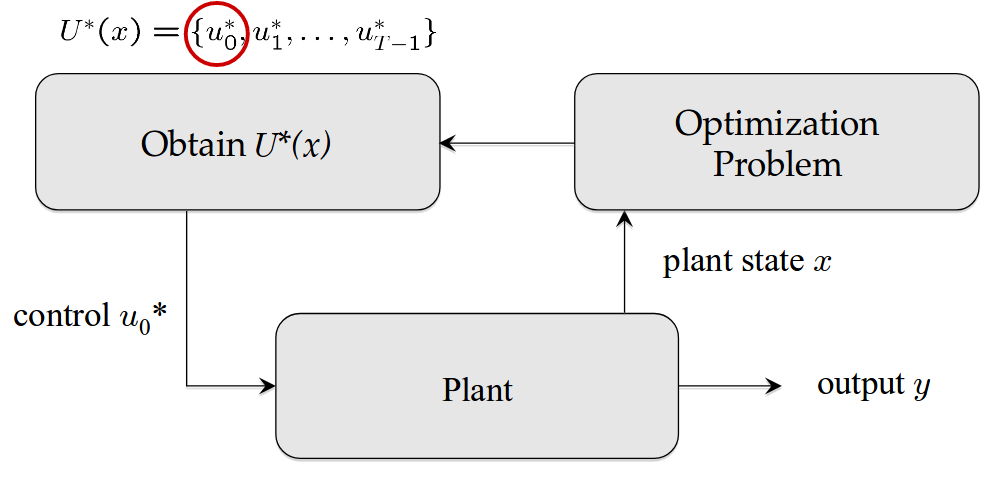
\includegraphics[width=350pt]{Abbildungen/mpcBlockDiagram.png}
  	\caption{Block Diagramm zu MPC}
  	\label{fig:mpcBlock}
  \end{figure}

Die Funktion lässt sich in drei Schritte unterteilen:
\begin{itemize}
	\item Zustandsschätzung \\ Im ersten Schritt wird der aktuelle Zustand des Systems erfasst und als Ausgangspunkt für die Berechnung des Optimierungsproblems festgelegt.
	\item Optimierung \\ In diesem Schritt werden die zukünftigen Zustände des Systems berechnet und welche Steuerparameter vonnöten sind, um eine Kostenfunktion zu minimieren. Diese entspricht im industriellen Umfeld zum Beispiel einer Optimierung der Fertigungsrate, der Kostenreduktion,  der Temperatursteuerung, etc.
	\item Steuerung \\ Die berechneten Steuerparameter werden zum Regeln des realen Systems angewandt. Danach wird wieder beim ersten Schritt fortgefahren.   
\end{itemize}


Die Stärke des \ac{MPC}-Ansatzes basiert auf der Prädiktion des Systemverhaltens. Ein präzises Vorhersagen setzt eine möglichst gute Systembeschreibung voraus. Je genauer diese an die Realität heranreicht, desto weiter in die Zukunft können die Systemzustände, ohne große Abweichung von der Realität, berechnet werden. Zudem kann das System näher an seine Systemgrenzen geführt werden. \\
Bei \ac{MPC} handelt es sich um ein Verfahren, welches immer bis zu einem festen Zeitpunkt in der Zukunft plant. Die Optimierung wird also immer für einen bestimmten Zeitraum $ [t_0, t_0 + T] $ durchgeführt . Der Bereich \(T\) wird in \(k\) Schritte unterteilt, für die jeweils ein Prädiktionsschritt berechnet wird. Dieser geht aus dem Zustand des vorherigen Schrittes $k -1$ und den dazu gehörigen Steuergrößen hervor. Nachdem der Optimierer die für eine Kostenfunktion idealen Steuergrößen für den gesamten Prädiktionsvektor berechnet hat, wird nur der \emph{erste} Steuerwert ausgewählt und zur Regelung im realen System eingesetzt. Der Zusammenhang aus Prädiktion und Kostenfunktion ist im Schaubild \ref{fig:mpcTheory} verdeutlicht. Für jeden Schritt im Vorhersagehorizont wird der Steuerparameter berechnet, der den Systemzustand möglichst schnell der vorgegebenen Trajektorie annähert. Das Wissen über das zu steuernde System hilft, die dafür passenden Steuerparameter zu finden und frühzeitig genug die Amplitude so anzupassen, dass kein Übersteuern auftritt. 

\begin{figure}[ht!]
	\centering
	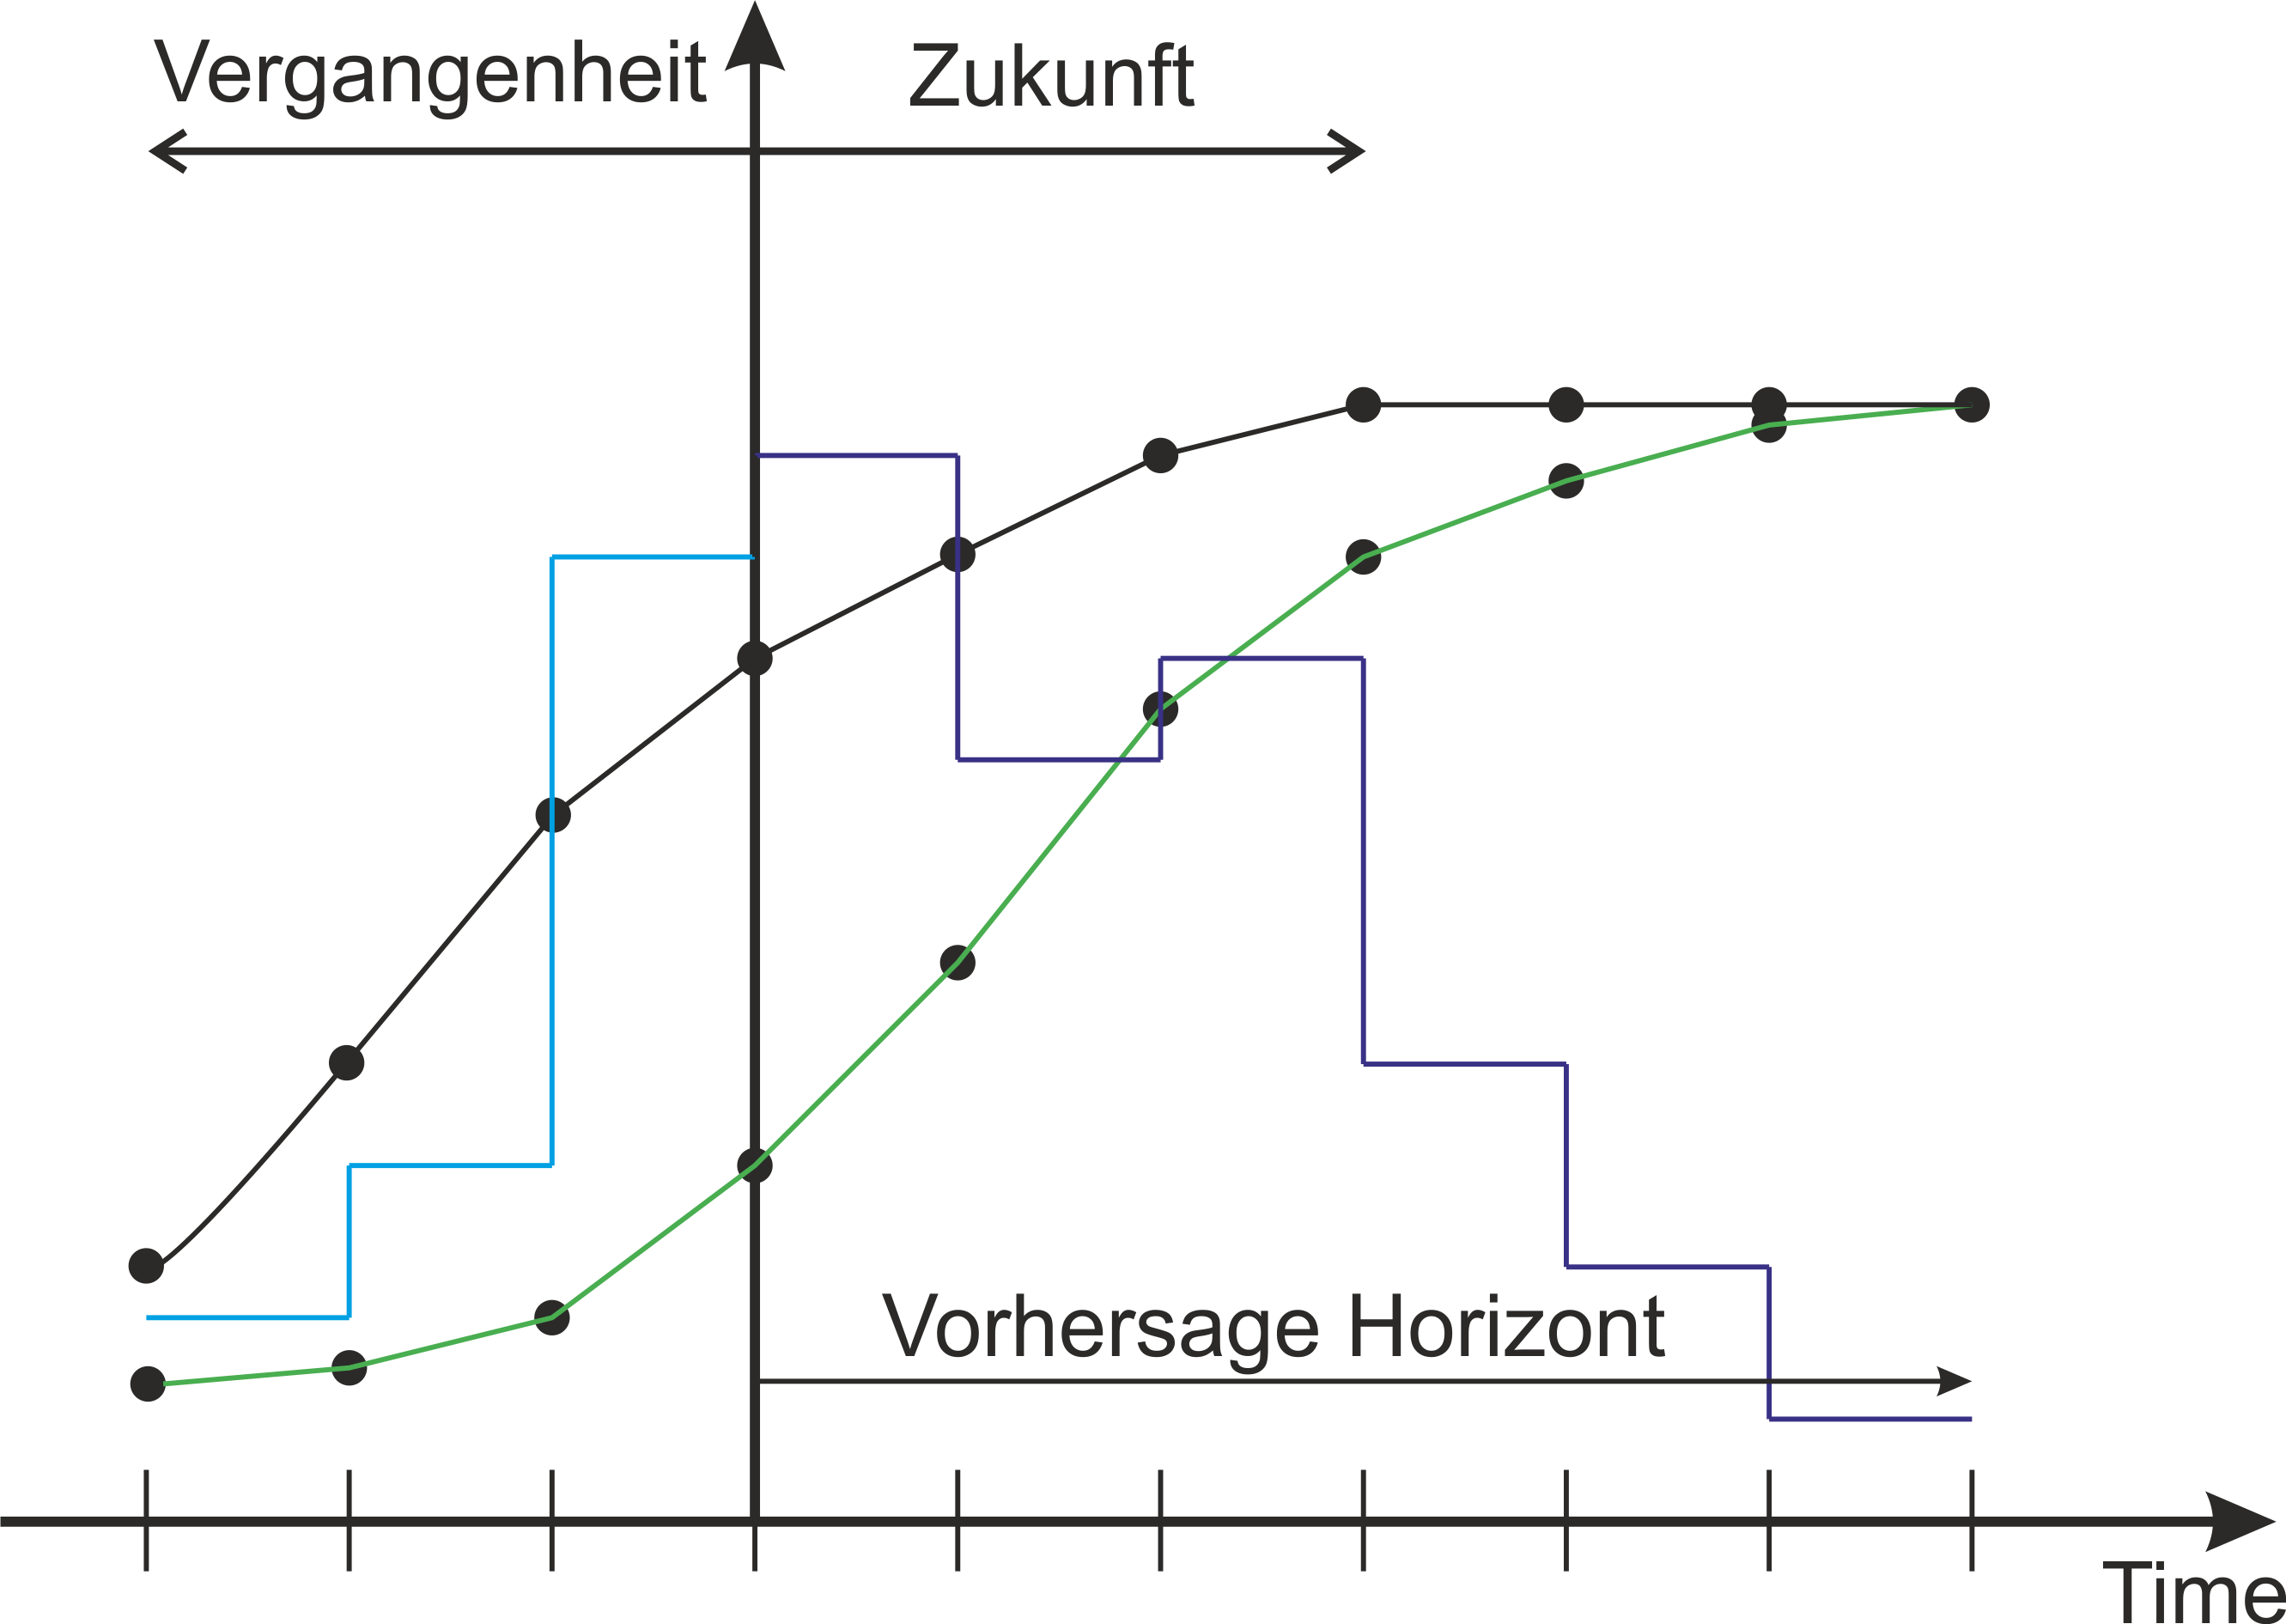
\includegraphics[width=400pt]{Abbildungen/mpcParadigm.png}
	\caption{Funktionsprinzip von \ac{MPC}: Die Kostenfunktion ist die Reduktion der Distanz zur Referenztrajektorie. Durch das Wissen über das hinterlegte Modell können die Kosten sehr schnell minimiert werden ohne die Beschränkungen zu verletzen}
	\label{fig:mpcTheory}
\end{figure}

Wie bereits ausgeführt wurde, berücksichtigt der \ac{MPC}-Ansatz auch Eingangs-, Ausgangs- und Zustandsbeschränkungen, mit denen der Suchraum einschränkt wird. Diese sind im Falle eines Rennautos zum Beispiel die maximale Geschwindigkeit, Lenkeinschlag, Beschleunigung und Bremskraft. Ebenfalls ein sehr gutes Beispiel für eine Zustandsbeschränkung ist die Reisequalität in einem normalen Straßenauto. Ruckartiges Anfahren und allgemein plötzliche Änderung der lateralen wie longitudinalen Beschleunigung trübt bei einem autonomen Fahrzeug das Fahrgefühl. Eine Möglichkeit diesem Problem zu begegnen ist die Begrenzung der Änderungsrate der Beschleunigung des Fahrzeugs.\\

Das Grundgerüst des \ac{MPC}-Ansatz bildet der Optimierer, der die optimale Lösung für die gewünschte Kostenfunktion sucht. Im Folgenden wird daher auf die Funktionsweise von diesem eingegangen.


\section{Optimierung}
Das Ziel der Optimierung besteht darin, eine gegebene Funktion \(f(\vec{x})\), auch als Kostenfunktion bezeichnet, zu mini- oder maximieren. 
Dies wird in einer Vielzahl von Anwendungsgebieten genutzt:
Zur Berechnung von Profit bzw. Verlust in einem Betrieb, der Geschwindigkeit oder Distanz in einem physikalischen Problem oder Beispielsweise die erwartete Kapitalrendite für eine Geldanlage.  
Die Bezeichnung lineare Programmierung bezieht sich auf die Lösung eines linearen  Optimierungsproblems und hat nichts mit dem eigentlichen Programm zu tun. 
Die allgemeine mathematische Definition eines Optimierungsproblems ist

\text{minimiere}  
\noindent\hspace*{3mm}%
$f(\vec{x}) $ \\
\text{unter Berücksichtigung von} 
\noindent\hspace*{3mm}%
$g_i(\vec{x})$ $\leq$ $0,$ $i=1,2,...,p$  \\
\noindent\hspace*{50mm}%
$h_j(\vec{x})= 0,$ $j= 1,2,...,m$\\ 
\noindent\hspace*{50mm}%


Der Eingabeparameter $\vec{x}$ sei aus $\mathbb{R} \textsuperscript{n} $, das heißt, das Problem hängt von \(n\) Einflussparametern ab. Die Zielfunktion $f:D \rightarrow \mathbb{R} $ sei zweifach stetig differenzierbar. Weiterhin sind die Nebenbedingungen in Ungleichheitsform $g_i:D \rightarrow \mathbb{R}$ mit $1\leq i \leq p$ und in Gleichheitsform $h_j:D \rightarrow \!R$ mit $1\leq j \leq m$ gegeben.
Wird \(f(\vec{x})\) durch \(-f(\vec{x})\) ersetzt, wird aus dem Mini- ein Maximierungsproblem. Der Unterschied zu einem nichtlinearen Programm ist, dass mindestens eine der Gleichungen des Optimierungsproblems nichtlinear ist.

Ein Optimierungsproblem hat nicht immer eine Lösung. Zum Beispiel können sich die  Ungleichungen, welche den Suchraum einschränken, widersprechen ($x \leq 0 $ und $x > 0$). Außerdem kann das Problem unbeschränkt sein. Soll zum Beispiel eine Optimierungsvariable minimiert werden, die nach unten nicht beschränkt ist, kann keine Lösung gefunden werden. 

Ein Optimierungsproblem lässt sich in Matrixschreibweise darstellen. Es besteht aus der Matrix $A \in \mathbb{R} \textsuperscript{m,n}$, die zusammen mit den Vektoren $b \in \mathbb{R} \textsuperscript{m,1}$ die Un- und Gleichheitsbedingungen enthält. Der Vektor $c \in \mathbb{R} \textsuperscript{1,n}$ kodiert die Zielfunktion. Gesucht wird also der Vektor $x \in \mathbb{R} \textsuperscript{n}$, der die Bedingungen

\[  \begin{array}{cccc}
a_{11} x_1 + & ... & + a_{1n} x_n & \leq b_1 \\   	
a_{21} x_1 + & ... & + a_{2n} x_n & \leq b_2 \\ 
. & . & . & . \\
. & . & . & . \\
a_{m1} x_1 + & ... & + a_{mn} x_n & \leq b_m \\
\end{array}\] 
erfüllt und gleichzeitig die Zielfunktion 
$cx=c_1 x_1 + ... + c_n x_n$ minimiert.
Die Kurzschreibweise für dieses Gleichungssystem ist: \\
\text{min} $\{ c\textsuperscript{T}x | Ax \leq b, x \geq 0 \}$

Veranschaulichen lässt sich die Lösung des Problems geometrisch im zweidimensionalen Raum, so dargestellt in Abbildung \ref{fig:linOpt}.

\begin{figure}[ht!]
	\centering
	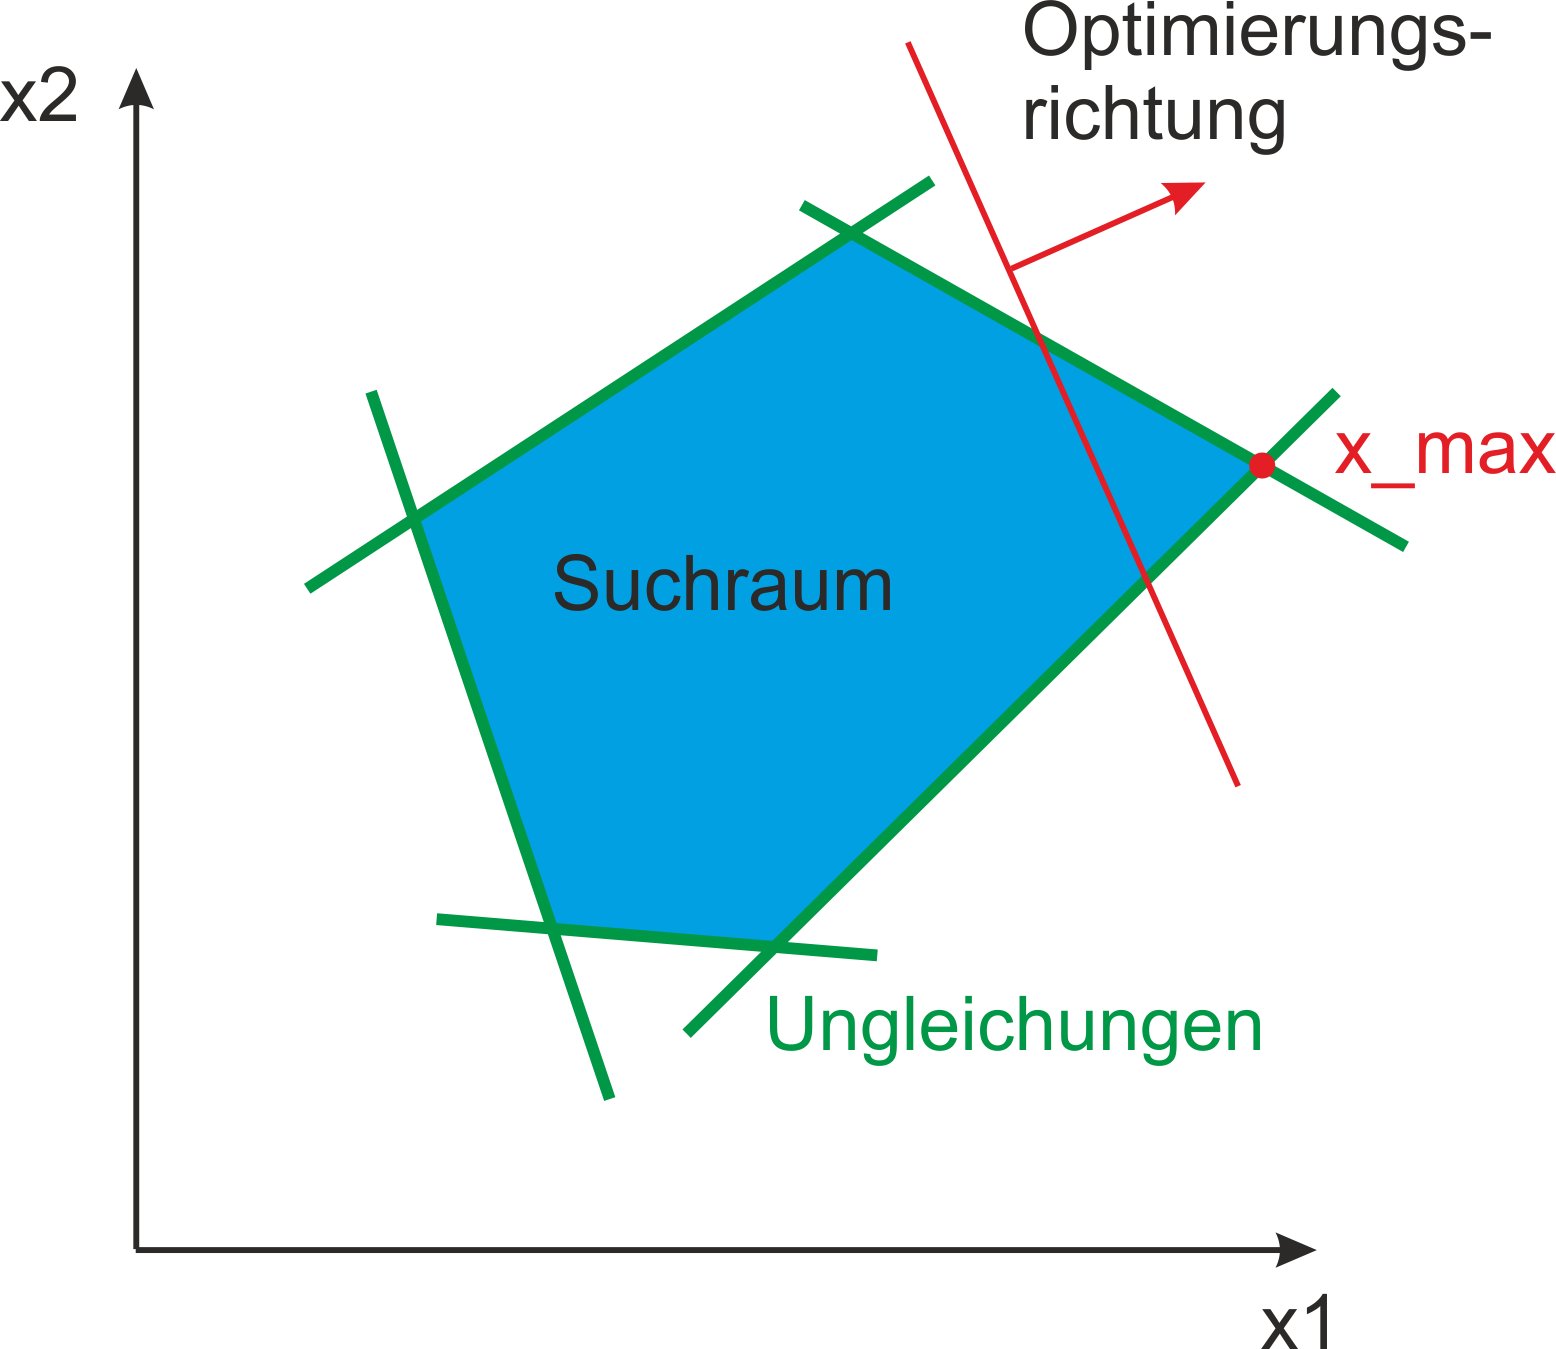
\includegraphics[width=300pt]{Abbildungen/linearOpt.png}
	\caption{Lineare Optimierung: Suche des Maximums an den Schnittpunkten der Ungleichungen}
	\label{fig:linOpt}
\end{figure}

Jede Ungleichung $a_i x \leq b_i$ teilt den Suchraum in zwei Hälften, eine mit zulässigen Punkten und eine ohne. Die Punkte auf der Grenze sind ebenfalls zulässig. Die Menge der Punkte, welche alle Ungleichungen erfüllt, ist genau der Schnitt dieser Halbräume. Dieser Bereich ist in Abbildung \ref{fig:linOpt} blau dargestellt. Der Punkt, der die Kostenfunktion $c: x \rightarrow c\textsuperscript{T} x$ minimiert, liegt auf den Kanten der Ungleichungen und wird durch Verschiebung der Hyperebene $ \{x| c\textsuperscript{T} x = 0 \}$ in Richtung des Vektors \(c\) gefunden. Nachdem das Optimierungsproblem aufgestellt ist, gibt es verschiedene Ansätze dieses zu berechnen.


\subsection{Simplex-Verfahren}
Bei der in dieser Arbeit zu lösenden Optimierung handelt es sich um ein nichtlineares Optimierungsproblem. Um dieses zu lösen, wird auf ein Innere-Punkte-Verfahren zurückgegriffen. Für ein besseres Verständnis des Verfahrens soll zuerst das Simplex-Verfahren kurz vorgestellt werden. Es wird für lineare Optimierungsprobleme eingesetzt und veranschaulicht die Suche nach der optimalen Lösung sehr gut. Das Verfahren wurde 1951 von Dantzig \cite{dantzig51} entwickelt und basiert auf dem Zusammenhang, dass ein lösbares lineares Programm immer einen Knoten besitzt, an dem sich Kanten verschiedener Ungleichungen treffen und die Kostenfunktion minimieren. Das Verfahren nutzt diese Eigenschaft aus, indem es sich iterativ von einem Eckpunkt zum nächsten bewegt. Das Verfahren ist bildlich in der Grafik \ref{fig:splxMethod} dargestellt.
\begin{figure}[ht!]
	\centering
	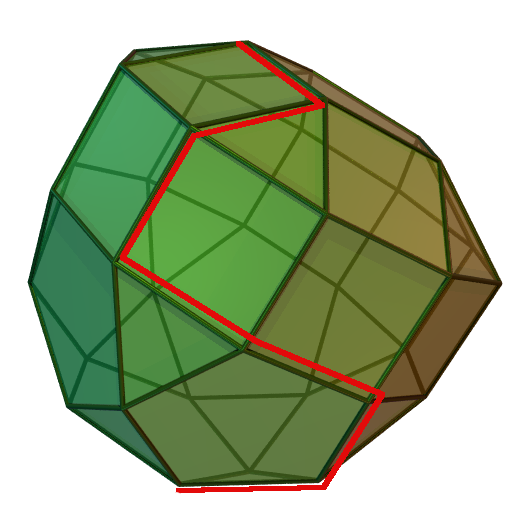
\includegraphics[width=200pt]{Abbildungen/simplexMethod.png}
	\caption{Simplex Methode: Ablaufen des Suchraums entlang der Kanten der Ungleichheitsbedingungen von Knoten zu Knoten}
	\label{fig:splxMethod}
\end{figure}

Die Kante, die gewählt wird, um sich zum nächsten Eckpunkt zu bewegen, hängt immer davon ab, auf welcher Flanke liegenden Punkte die Kostenfunktion weiter minimieren. Kann keine weitere Flanke gefunden werden, die die Kosten weiter reduziert, endet das Verfahren im Optimum. Die Anzahl der Kanten im Polyeder wächst exponentiell mit der Anzahl der Optimierungsvariablen (n). Da im schlechtesten Fall der Simplex-Algorithmus jeden Knotenpunkt einmal betrachten muss, hat das Verfahren daher ein exponentielles Wachstum $\mathcal{O}(c\textsuperscript{n})$ mit $c>1$ \cite{doi:10.1137/S0036144502414942}. Trotz dieser Problematik hat das Simplex-Verfahren in der Praxis eine sehr gute Laufzeit und kann für den wiederholten Aufruf einer nur leicht veränderten Optimierung (Anpassen von Parametern nach dem letzten Aufruf) einen sogenannten Warmstart nutzen. Dieser beschleunigt die Lösung ebenfalls deutlich.\\


\subsection{Innere-Punkte-Verfahren} 
\label{ipm} 
Die Suche nach noch besseren Verfahren, deren Komplexität nur polynomial mit der Dimension anwächst, führte dann in den Jahren 1979 bis 1984 zur Entwicklung eines neuen Algorithmus. Dieser wird als Innere-Punkte-Verfahren bezeichnet und eignet sich auch für nichtlineare Probleme. Die Un- und Gleichheitsbedingungen wie auch die Kostenfunktionen die im \ac{MPC}-Ansatz zum Regeln des Rennautos vorkommen, sind nichtlinear. Sie setzen daher einen Optimierer voraus, der diese Problemen berechnen kann. Zusätzlich gibt es, wie im Kapitel \ref{MPC} erwähnt, Beschränkungen, die bei der Suche der Lösung eingehalten werden müssen. Das Innere-Punkte-Lösungsverfahren erfüllt diese Anforderung für lineare, quadratische und nichtlineare Optimierungsprobleme und wird im Folgenden kurz vorgestellt. Der Ansatz des Verfahrens ist die Bewegung im Inneren des zulässigen Lösungsbereiches und nicht auf den Kanten wie beim Simplex-Verfahren. Diese Bewegung durch das Innere des Polytop ist in Abbildung \ref{fig:iterPointMethod} veranschaulicht.  
\begin{figure}[ht!]
	\centering
	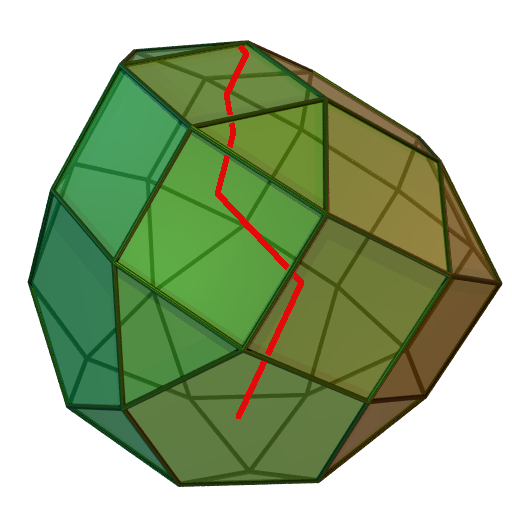
\includegraphics[width=200pt]{Abbildungen/iterPointMethod.png}
	\caption{Beim Innere-Punkte-Verfahren bewegt sich der Optimierer durch das Innere des Polytops auf der Suche nach dem Mimimum}
	\label{fig:iterPointMethod}
\end{figure}

Um dieses Verfahren umzusetzen, werden die Ungleichheitsbedingungen $g(\vec{x}) \geq 0$ der Standardform mit Hilfe einer Substitution so umgeformt, dass sie der Form $c(\vec{x}) = 0$ und $\vec{x} \geq  0$ entspricht. Die neue Ungleichheitsbedingung kann nun mit einem logarithmischen Strafterm $ \mu \ln x $  ersetzt und in die Kostenfunktion integriert werden. 
Der Faktor $\mu$ wird genutzt, um die Gewichtung des Strafterms zu verändern.

Die daraus resultierende Funktion wird als Barrierefunktion bezeichnet und ist definiert als \\
\begin{equation}
	B(x,\mu) =  c\textsuperscript{T}x - \mu \sum_{i}^{n} \ln x_i
\end{equation}
mit $\mu > 0$ und ersetzt die Kostenfunktion im ursprünglichen Optimierungsproblem. Der Strafterm verhindert, dass der Optimierer, wie beim Simplex-Verfahren, an den Grenzen der Un- und Gleichheitsbedingungen nach der Lösung sucht, sondern sich immer im Inneren des zulässigen Lösungsbereiches bewegt. Wird \(\mu\) sehr klein (tendiert gegen null), entspricht die Lösung des Barriereproblems der gleichen wie beim ursprünglichen Optimierungsproblem. Diese Eigenschaft wird genutzt, von einem großen \(\mu\) als Startpunkt iterativ $B(x,\mu)$ zu optimieren und dann vor der nächsten Iteration \(\mu\) zu verkleinern. Das schrittweise verkleinern von $\mu$ dient dazu, sich anfangs grob und schnell, später mit kleinen Schritten und langsam der Lösung zu nähern. Die Auswirkung der stetigen Verkleinerung von \(\mu\) ist in der Abbildung \ref{fig:iterPointLn} veranschaulicht.

\begin{figure}[ht!]
	\centering
	\begin{tikzpicture}
\begin{axis}[
width = 0.8\textwidth,
height = 0.5\textwidth,
ymin=-10,
ymax= 20,
ylabel=Barrierefunktion $-\mu \ln(x)$,
xlabel=Variable(x),
legend pos=north east]
\addplot [color=black, line width=0.5mm] table [x index=0, y index=1]{Data/barrierFunc.dat};
\addplot [color=blue, line width=0.5mm] table [x index=0, y index=2]{Data/barrierFunc.dat};
\addplot [color=green, line width=0.5mm] table [x index=0, y index=3]{Data/barrierFunc.dat};
\addplot [color=yellow, line width=0.5mm] table [x index=0, y index=4]{Data/barrierFunc.dat};
\addplot [color=orange, line width=0.5mm] table [x index=0, y index=5]{Data/barrierFunc.dat};
\addplot [color=red, line width=0.5mm] table [x index=0, y index=6]{Data/barrierFunc.dat};

\addlegendentry{$-0.0 \ln(x)$};
\addlegendentry{$-0.1 \ln(x)$};
\addlegendentry{$-1.0 \ln(x)$};
\addlegendentry{$-2.0 \ln(x)$};
\addlegendentry{$-5.0 \ln(x)$};
\addlegendentry{$-10.0 \ln(x)$};


\end{axis}
\end{tikzpicture} 
	\caption{Auswirkung des Parameters $\mu$ auf das Verhalten der Barrierefunktion}
	\label{fig:iterPointLn}
\end{figure}

Um die Lösung in jedem dieser iterativen Schritte zu finden, wird die Ableitung der Barrierefunktion gleich null gesetzt, da in diesem Punkt ein (lokales) Minimum existiert. Um diesen Punkt möglichst schnell zu finden, wird das Newton-Raphson-Verfahren angewandt. Bei diesem handelt es sich um eine Nullstellensuche, welche unter Zuhilfenahme der Ableitung der Funktion möglichst schnell ein Ergebnis findet. Der Algorithmus benötigt daher die Hesse-Matrix der Barrierefunktion. Die Berechnung dieser wird durch eine automatische Ableitung realisiert.

\subsection{Automatische Ableitung} 

Ableitungen sind eine Grundvoraussetzung für viele numerische Algorithmen. Die Genauigkeit und Geschwindigkeit der Berechnung ist jedoch oftmals problematisch.

Ein möglicher Ansatz die Ableitung 
\begin{equation}
	\Delta{\tiny } f(x) = (\frac{\partial f}{\partial x_1} (x), ..., \frac{\partial f}{\partial x_n})
\end{equation}
der Funktion $f:\Re \textsuperscript{n} \rightarrow \Re $ zu berechnen ist \\
\begin{equation}
	f'(x) \approx \frac{f(x+h) - f(h)}{h}
\end{equation}
 mit $ h \rightarrow 0$.
Dieser Ansatz ist jedoch mit einer Komplexität von $\mathcal{O}(n)$ sehr ineffizient. Es entstehen zudem Rundungsfehler \cite{julDiff}.
Eine andere Möglichkeit wäre die Ableitung manuell zu berechnen, was jedoch für komplexere Systeme sehr aufwendig und vor allem fehleranfällig ist. Eine bessere Lösung ist die automatische Ableitung (eng.: automatic differentiation). 
Dieses System kann die Ableitung bis auf die maximal mögliche Genauigkeit eines float-Datentyps berechnen. Zu der höheren Präzision kommt noch die deutlich bessere Laufzeit hinzu. Im Idealfall entspricht die Komplexität $\mathcal{O}(1)$ \cite{julDiff}. Um diese Vorteile nutzen zu können, wird jedoch ein genaues Wissen über die abzuleitende Funktion \(f(x)\) benötigt. Realisiert wird dies durch den Zugriff auf den Sourcecode der Methode oder durch ein Überladen der Operatoren. Das Verfahren ist abhängig von den Möglichkeiten der Programmiersprache und welcher Ansatz bei der Implementierung der automatischen Ableitung verfolgt wurde. \\

Ein Verfahren der Umsetzung ist der Vorwärtsmodus. Dieser basiert auf der Kettenregel 
\begin{equation}
	(f \circ g)' = (f' \circ g)g'
\end{equation}

Um dies auszunutzen wird eine abzuleitende Funktion $ y = f(g(h(x)))$ in seine Bestandteile $y = f(g(h(w_0))) = f(g(w_1)) = f(w_2) = w_3$ aufgetrennt und anschließend in die Kettenregel eingesetzt. 
\begin{equation}
\frac{\partial y}{\partial x} = \frac{\partial y}{\partial w_2} \frac{\partial w_2}{\partial w_1} \frac{\partial w_1}{\partial x}
\end{equation}
Zum besseren Verständnis wird die Ableitung $\frac{\partial y}{\partial x_1}$ für die Funktion
$y = f(x_1, x_2) = x_1x_2 + \sin(x_1)$  berechnet.\\
Dazu werden, wie oben bereits beschrieben, zuerst die Bestandteile substituiert:\\
$y = w_1w_2 + \sin(w_1) $ \\
$y = w_3 + w_4$ \\
$y = w_5$

Danach muss der Seed errechnet werden. Er kodiert über welche Variable (hier $x_1$) differenziert werden soll. Für $x_1$ ist der Seed $\dot{w_1} = \frac{\partial x_1}{\partial x_1} = 1$ und   $\dot{w_2} = \frac{\partial x_2}{\partial x_1} = 0$.
Im letzten Schritt werden nur noch von innen nach außen die Substitutionen ersetzt. \\
$\dot{w_3} = w_2\dot{w_1} + w_1 \dot{w_2}$ \\
$\dot{w_4} = \cos{w_1} \cdot \dot{w_1}$ \\
$\dot{w_5} = \dot{w_3} + \dot{w_4}$ \\
Dieses Verfahren kann im sogenannten Rückwärtsmodus auch von außen nach innen berechnet werden.  

\newpage
\section{Fahrzeugmodelle}
Nachdem die Grundlagen zur Optimierung gelegt wurden, wird nun auf den Teil im \ac{MPC}-Algorithmus eingegangen, welcher die Un- und Gleichheitsbedingungen definiert.
Wie der Name Model Predictive Control schon andeutet, wird eine Modellbeschreibung des zu regelnden Systems benötigt. Diese wird genutzt, um zukünftige Zustände zu berechnen und bildet damit einen wichtigen Bestandteil des Verfahrens. Je genauer die Beschreibung das reale System approximiert, desto besser ist die Vorhersage und damit auch die Regelung des Fahrzeugs.
Im Folgenden wird zuerst ein kinematisches Fahrzeugmodell eingeführt und dann zu einem dynamischen Modell erweitert.   

\subsection{Kinematisches Modell}
\label{kinematicModel}
Unter gewissen Einschränkungen kann ein kinematisches Modell die laterale und longitudinale Bewegung eines Fahrzeugs mathematisch beschreiben. In diesem sehr stark vereinfachten Modell werden für die Berechnung der Bewegung keine wirkenden Kräfte berücksichtigt, sondern nur die geometrischen Beziehungen des Fahrzeugs betrachtet. \\
Im ersten Schritt werden die jeweils an einer Achse verbundenen Räder zu einem einzigen zusammengefasst. Diese Vereinfachung wird als Bicycle Modell bezeichnet und vereinfacht die Berechnungen \cite{BicycleModel}. Obwohl auch für Hinterradlenkung möglich, wird im Folgenden nur die Vorderradlenkung betrachtet, da das Rennauto des High-Octane Motorsport e.V. keine Hinterradlenkung besitzt. Die Lenkwinkel, welche durch das Bicycle Modell berechnet werden, entsprechen nicht den Lenkwinkeln am echten Fahrzeug. Die kurveninneren und kurvenäußeren Räder bewegen sich auf zwei Kreisen mit unterschiedlichen Radien und damit auch verschiedenen Anstellwinkeln. Dies wird in Fahrzeugen durch die Ackermann-Lenkung mechanisch umgesetzt \cite{rajamani2011vehicle}.


Die nichtlinearen, zeitkontinuierlichen Gleichungen 

\begin{eqnarray}
\label{eq:kinDiscrete}
\dot{x}   &= &v  \cos(\psi + \beta)\\
\dot{y}   &= &v  \sin(\psi + \beta)\\
\dot{\psi} &= &\frac{v}{l_r} \sin(\beta) \\
\dot{v}    &= &a \\
\beta      &= &\arctan \left( \frac{l_r}{l_f + l_r} \tan(\delta_f) \right) \label{compute_beta}
\end{eqnarray}
basieren auf \cite{rajamani2011vehicle, 7225830} und beschreiben das kinematische Modell bezüglich eines Inertialsystems (siehe Abbildung \ref{fig:kinmodel}), in dem \(x\) und \(y\) die Koordinaten des Schwerpunktes im Inertialsystem darstellen.
\\
\begin{figure}[ht!]
	\centering
	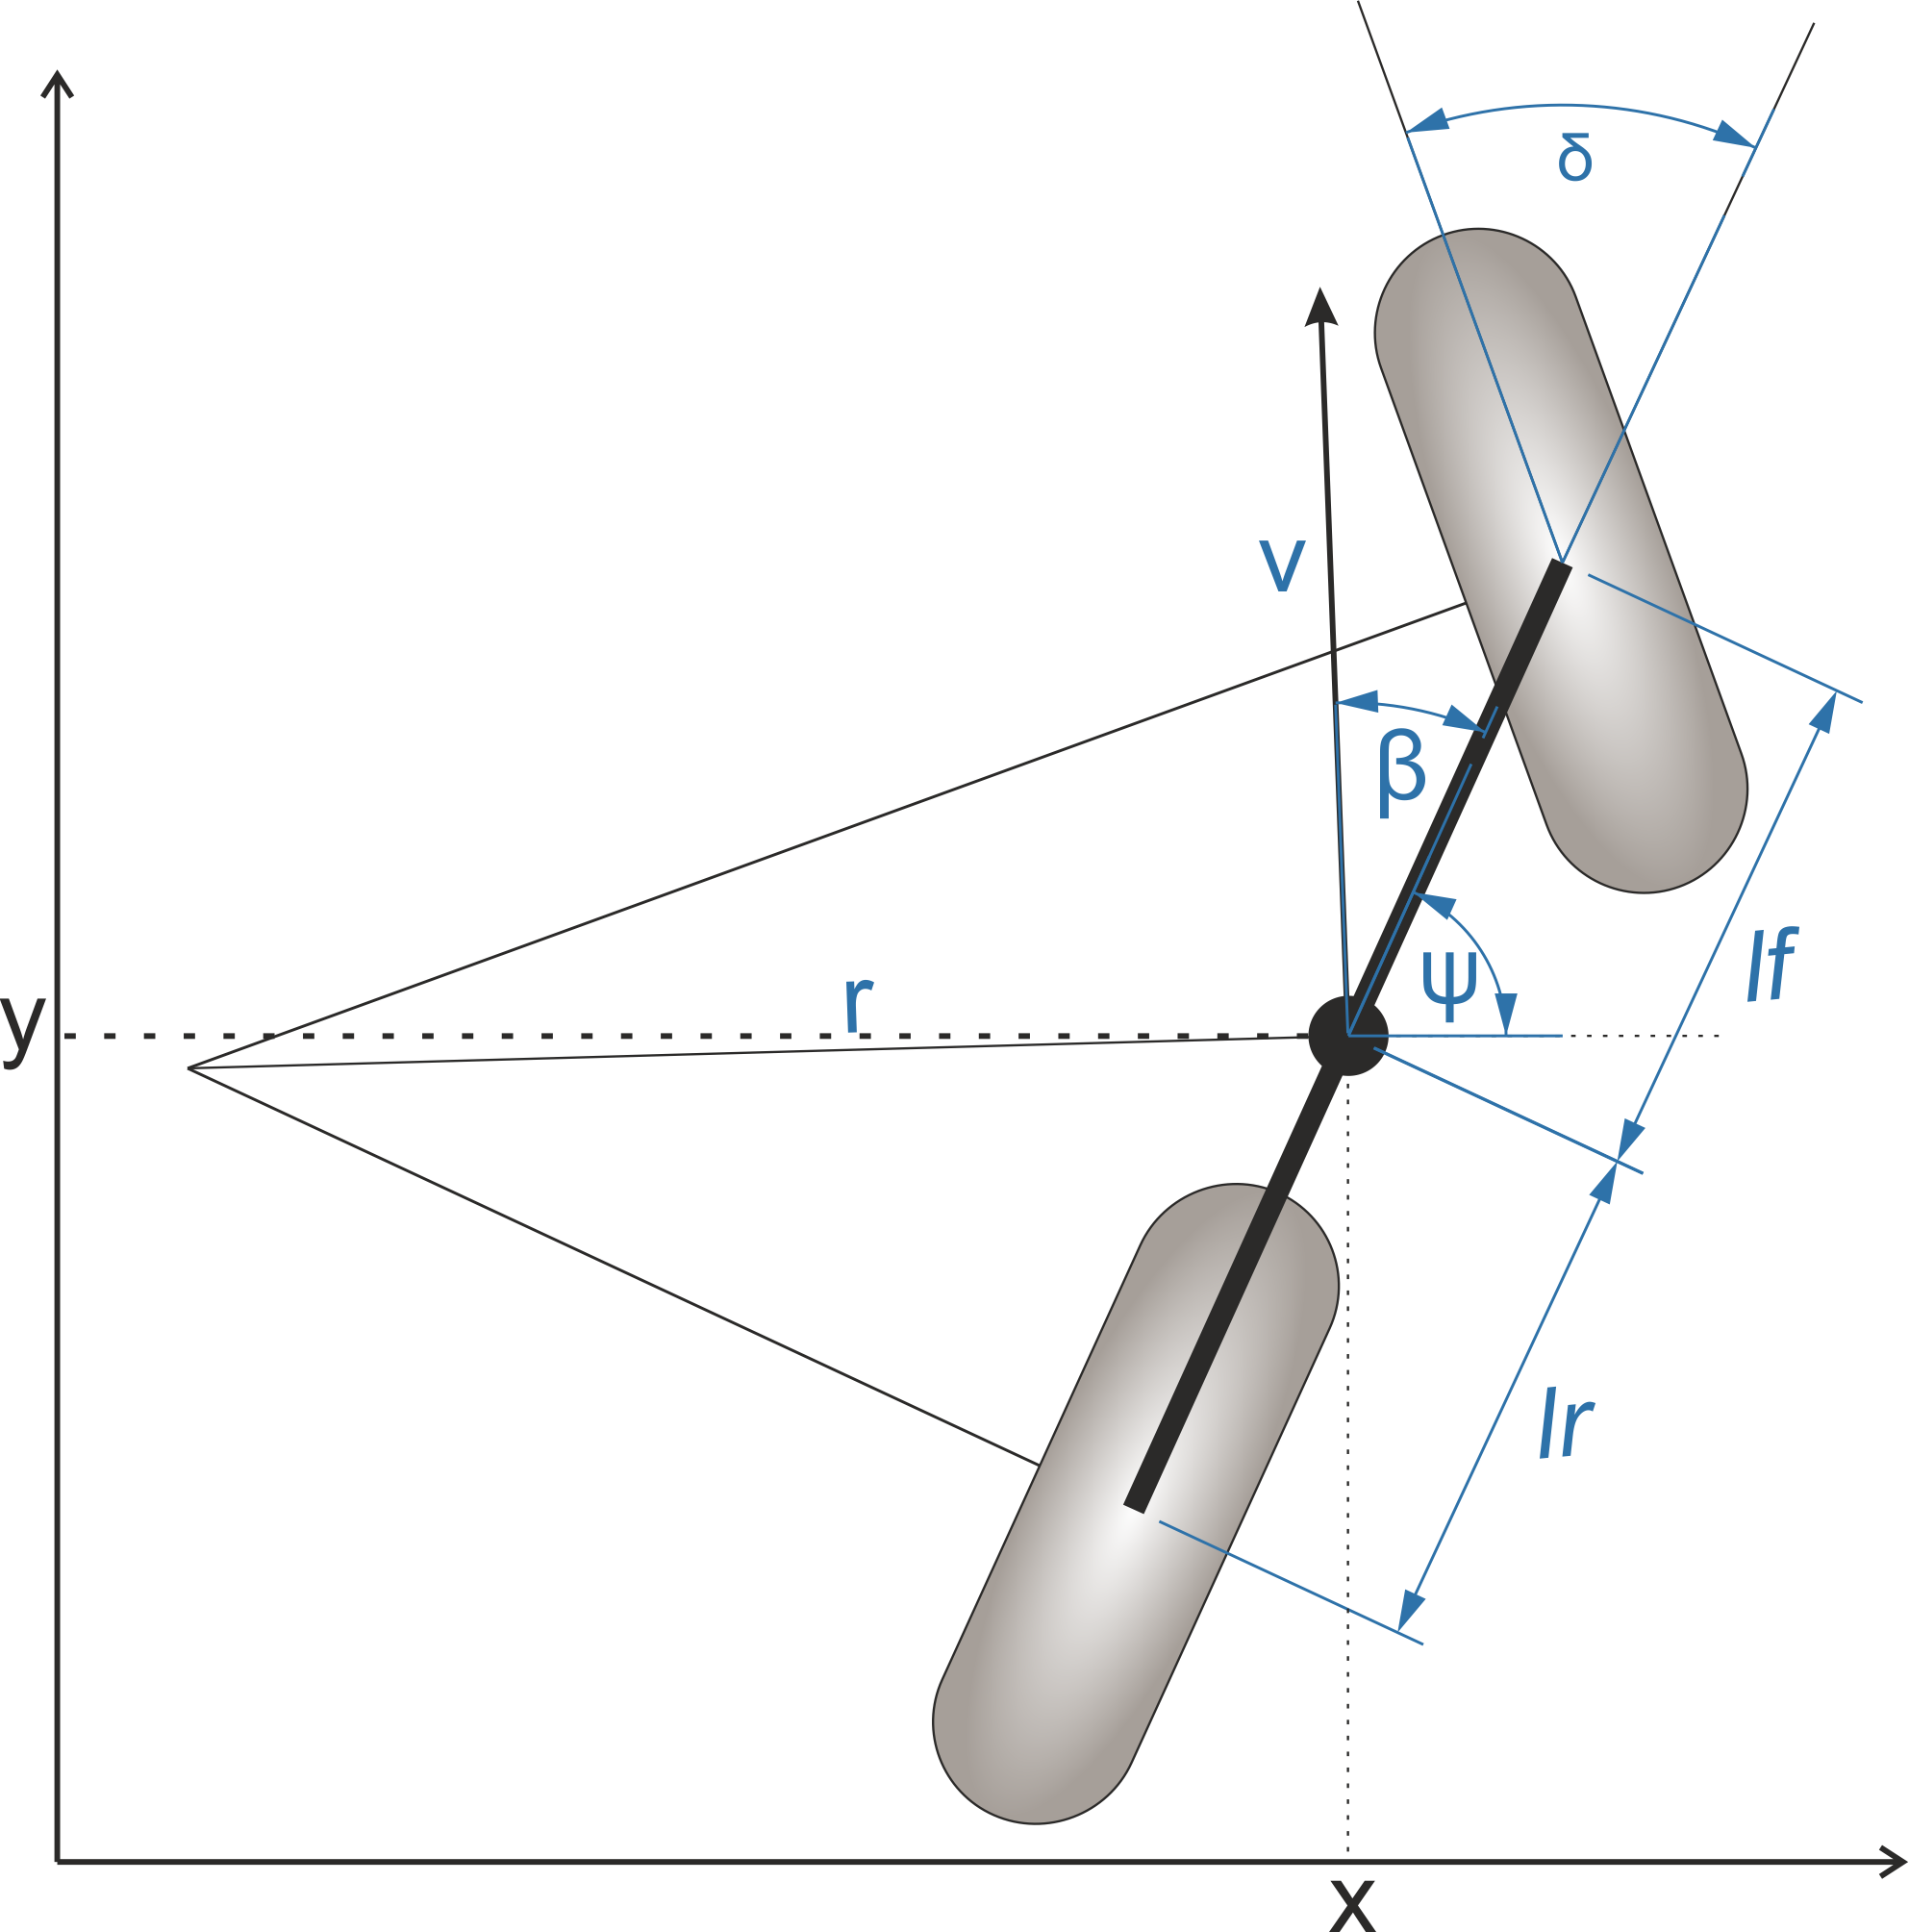
\includegraphics[width=250pt]{Abbildungen/kinBicycle.png}
	\caption{Kinematisches Modell}
	\label{fig:kinmodel}
\end{figure}
 
\(\psi\) ist die Orientierung und \(v\) die Geschwindigkeit des Fahrzeugs. \(l_f\) und \(l_r\) sind die Abstände der vorderen (\(l_f)\) und hinteren (\(l_r)\) Achsen zum Schwerpunkt.
Der Schwimmwinkel \(\beta\), ist der Winkel  zwischen der Bewegungsrichtung des Fahrzeugs im Schwerpunkt und der Fahrzeuglängsachse bei der Kurvenfahrt. Die Beschleunigung \(a\) bezieht sich ebenfalls auf den Schwerpunkt und zeigt immer in die Richtung des Geschwindigkeitsvektors. Wird der Lenkeinschlag ruckartig geändert, verändert sich auch genauso ruckartig der Geschwindigkeitsvektor. Dies ist einer der Nachteile des kinematischen Modells.\\
Die Parameter lassen sich in zwei Bereiche unterteilen:

\begin{itemize}
	\item Steuerparameter  \\
	\(a\), \(\delta\)
	\item Zustandsgrößen \\
	\(x\), \(y\), \(v\), \(\psi\)
	
\end{itemize}


Die Annahme eines kräftefreien Modells, bei dem das Vorderrad genau in die Richtung rollt, in die es zeigt, ist nur bis etwa $5$ $ \frac{\text{m}}{\text{s}}$ plausibel \cite{rajamani2011vehicle}. Danach müssen die Kräfte, welche die Reifen auf die Straße übertragen können, mitbetrachtet werden. Diese werden dann im dynamischen Modell genutzt, um eine genauere Vorhersage berechnen zu können.

Die für das kinematische Modell angenommenen Werte stammen vom Fahrzeug des High-Octane Motorsports Verein (siehe \ref{vehicleParam}). Die Beschleunigung \(a\) wurde für einen Acceleration Durchgang mit der Zeit $t = 4,5$ s und der Endgeschwindigkeit $v = 33,6$ $\frac{\text{m}}{\text{s\textsuperscript{2}}}$  ($121$  $\frac{\text{km}}{\text{h}}$) berechnet. Nach einsetzen in die Gleichung zum Berechnen der Geschwindigkeit 
\begin{equation}
a = \frac{v}{t}  \label{long_acc_kin}
\end{equation}
ergibt sich eine mittlere Beschleunigung von $7,47$ $ \frac{\text{m}}{\text{s\textsuperscript{2}}}$ .


\subsubsection*{Begrenzung des Kurvenradius}
\label{betaMax}
Da beim kinematischen Modell die Annahme getroffen wird, dass das Rad immer in genau die Richtung rollt, in die es zeigt, kann das Fahrzeug bei jeder Geschwindigkeit \(v\) den gleichen Kurvenradius durchfahren. Um auch in höheren Geschwindigkeiten eine akzeptable Regelung zu erhalten, wird eine Beschränkung eingefügt, die die maximale Querbeschleunigung beschränkt. Der Maximalwert entspricht dem höchsten g-Wert, den das Fahrzeug des High-Octane Motorsports mit Aerodynamik in einer Kurve erreichen kann: $a_{max} \sim 2,0$ g. 
Mit der Gleichung
\begin{equation}
	|\beta| \leq \arctan \left(\frac{l}{4} \frac{a_{max}}{v^2} \right) \label{limitLatAcc}
\end{equation}
wird dies über die Einschränkung des Schwimmwinkels, der wiederum aus dem Lenkwinkel (\ref{compute_beta}) berechnet wird, erreicht. Bei höheren Geschwindigkeiten wird also der minimale Kurvenradius durch die künstliche Limitierung des maximalen Lenkwinkels erreicht. 


\subsection{Reifenmodell}
\label{tireModel}
Da der Reifen der einzige Kontaktpunkt zwischen Fahrbahn und Fahrzeug ist, beeinflusst er das Fahrverhalten maßgeblich. Aufgabe des Reifens ist es, sämtliche Kräfte und Momente zu übertragen und eine optimale Straßenlage zu gewährleisten. Demzufolge ist der Reifen das Bauteil, das die Fahrleistungen des Rennautos am stärksten beeinflusst.

Die Kräfte, die ein Reifen auf die Straße übertragen kann, sind in longitudinalen und lateralen Anteil aufgespalten. Sie hängen ab von der Radlast, die das Fahrzeug auf die Straße presst, dem Schlupf und dem Schräglaufwinkel. Die Radlast \(F_z\) berechnet sich aus der Normalkraft und der Radlastverteilung und wird im Folgenden als konstant angesehen. Der Schlupf tritt in longitudinaler Richtung auf und ist die Differenz aus Umlaufgeschwindigkeit und Bewegungsgeschwindigkeit des Fahrzeugs.
Nur wenn ein Schlupf vorhanden ist, übertragen Reifen Kraft auf ihren Untergrund. Dies ist bei Beschleunigungsrennen gut zu beobachten, wo die maximale Kraftübertragung im Bereich von 30 Prozent Schlupf liegt (leicht durchdrehende Reifen).
Die Seitenführungskraft \(F_y\) wirkt bei einer Kurvenfahrt der Fliehkraft entgegen und hält das Fahrzeug auf der Spur solange ein Kräftegleichgewicht besteht. Für diese laterale Kraft muss der Schräglaufwinkel, genauso wie beim Schlupf, größer null sein. Als Schräglaufwinkel wird der von der Radmittelebene \(\delta\) (Lenkwinkel) und der Bewegungsrichtung \(\theta_{vf}\) des Reifens eingeschlossenen Winkel (siehe Abbildung \ref{fig:linLat})

\begin{equation}
\alpha_f = \delta - \theta_{vf}
\end{equation}
bezeichnet. Der gleiche Zusammenhang gilt auch für das hintere Rad, welches jedoch in unserem Fall nicht gelenkt wird
\begin{equation}
\alpha_r = \theta_{vr}
\end{equation}


\begin{figure}[ht!]
	\centering
	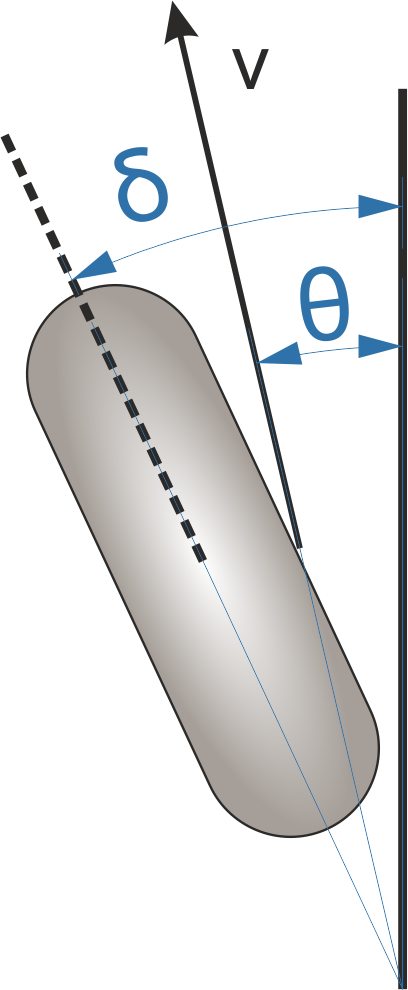
\includegraphics[width=70pt]{Abbildungen/slipAngle.png}
	\caption{Der Schräglaufwinkel ergibt sich aus Lenkwinkel \(\delta\) und Bewegungsrichtung \(\theta_{v}\)}
	\label{fig:linLat}
\end{figure}


Für kleine Schräglaufwinkel besteht ein linearer Zusammenhang aus lateraler Kraft und Winkel.
\begin{eqnarray}
F_{yf} = C_\alpha \alpha_f \\
F_{yr} = C_\alpha \alpha_r
\end{eqnarray}

Für größere Schräglaufwinkel kann kein linearer Verlauf mehr angenommen werden und es muss eine genauere Approximation der Kräfte gewählt werden. Hierfür wird die sogenannte \ac{M.F.}  \cite{magicFormula} verwendet. Dabei handelt es sich um eine mathematische Gleichung, die sehr gut Messkurven approximiert, die auf Testständen gemessen werden.
Sie wurde 1993 von Pacejka und Bakker entwickelt und eignet sich sowohl für die Berechnung der longitudinalen, wie auch der lateralen Kräfte. 
Die Querkräfte $F_y$, die der Reifen auf die Straße überträgt, ergeben sich durch den Schräglaufwinkel $\alpha$.

\begin{equation}
F_y =  D\sin(C\arctan(B\alpha - E(B\alpha - \arctan(B\alpha))))  \label{eq:magicF} 
\end{equation}

Die Gleichung hängt von den Faktoren \(C\), \(B\) und \(E\) ab. 
\begin{eqnarray}
C =& 1 + \left(1- \left(\frac{2}{\pi} \arcsin \left(\frac{y}{D} \right) \right) \right) \\
B =& \frac{\tan(beta)}{CD} \\
E =& \frac{ B  x_m - \tan \left(\frac{pi}{2 C} \right)}{Bx_m - \arctan(Bx_m)}
\end{eqnarray}


Diese werden abhängig von den folgenden Parametern berechnet.

\begin{itemize}
	\item $D$ \\	
	Die maximale Kraft, die der Reifen im höchsten Punkt übertragen kann
	\item $beta$\\
	Die Steigung im linearen Bereich 
	\item $x_m$ \\
	Der Punkt in rad, in dem die maximale Kraft übertragen wird
	\item $y_a$ \\
	Die maximale Kraft, gegen die die Kurve für große Schräglaufwinkel tendiert 
\end{itemize}

Die Parameter ändern sich mit der Normalkraft, die das Fahrzeug auf die Straße presst. Ist sie konstant wie in unserem Fall, müssen die Werte nur einmal berechnet werden und bleiben danach unverändert. Sie unterscheiden sich jedoch für das vordere $(.)_f$ und hintere Rad $(.)_r$. Werden in einem komplexeren Modell auch die aerodynamischen Abtriebskräfte und die Steigung der Straße berücksichtigt, ändern sich $D$, $beta$, $xm$ und $y_a$ mit jeder Veränderung der Normalkraft, was die Neuberechnung von C,B und E zur Folge hat. Zur besseren Veranschaulichung ist in der Zeichnung \ref{fig:tireModelParameter} der Einfluss der einzelnen Werte auf die Kurve der Reifenkräfte dargestellt. 

\begin{figure}[ht!]
	\centering
	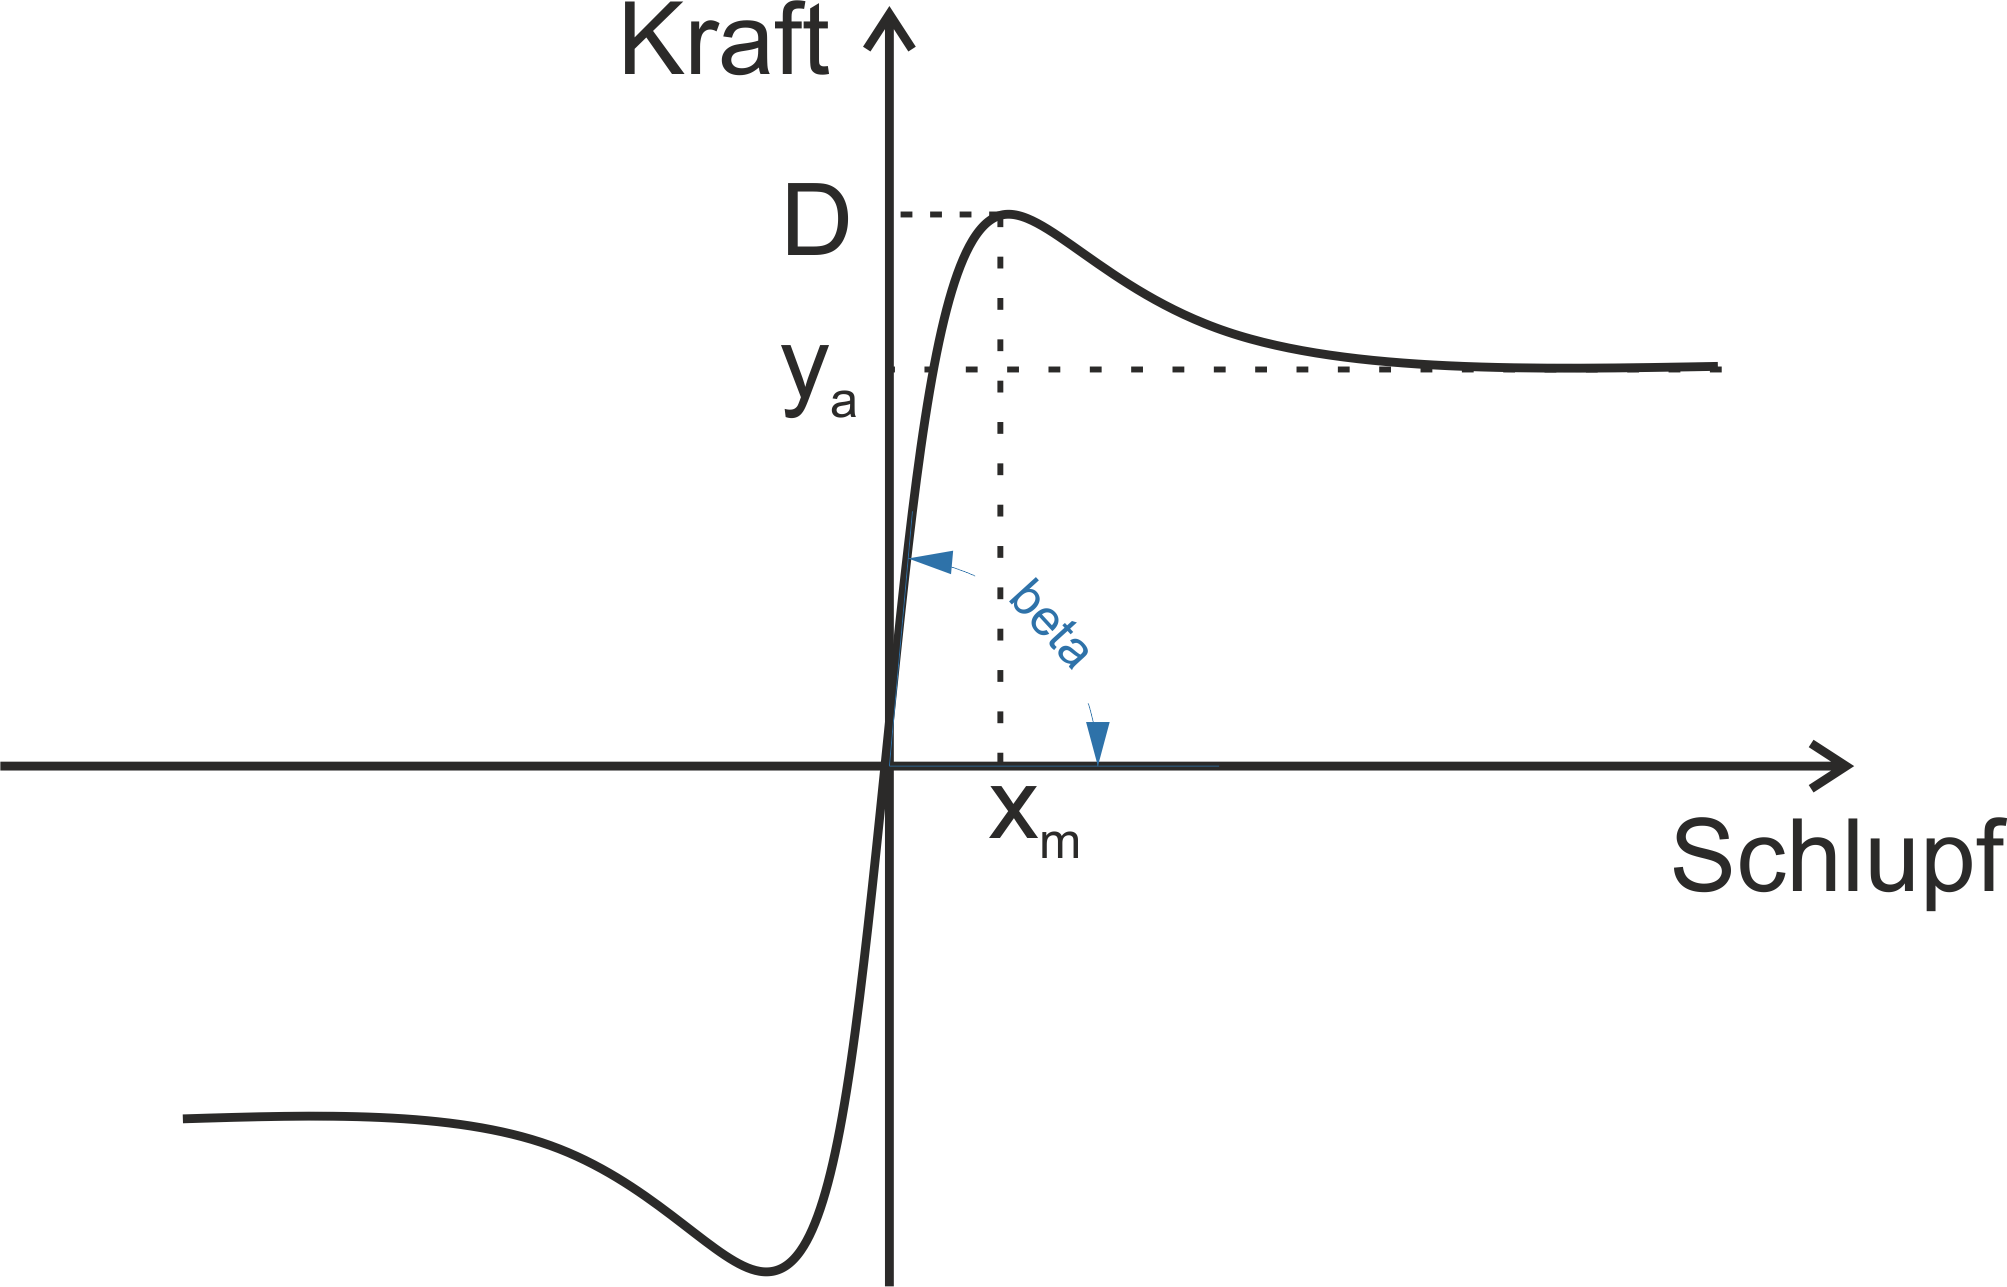
\includegraphics[width=350pt]{Abbildungen/tireModel.png}
	\caption{Parameter im Reifenmodell}
	\label{fig:tireModelParameter}
\end{figure}
 
Zusätzlich zu dem ursprünglichen Reifenmodell wird eine Vereinfachung betrachtet, die weniger Rechenaufwand erzeugt. Es wird eine lineare Funktion für die maximale laterale Kraft
\begin{equation}
F_y = C \alpha 
\end{equation}
angenommen, die durch die Maximalkraft $|F_y| <= F_{max} $ beschränkt ist.
Nachteil der Vereinfachung ist die geringere Genauigkeit. 
Die zwei Modelle sind in der Abbildung \ref{fig:pacejka}
\begin{figure}[ht!]
	\centering
	\begin{tikzpicture}
\begin{axis}[
width = 0.8\textwidth,
height = 0.5\textwidth,
xlabel=Schräglaufwinkel in rad,
ylabel=Laterale Seitenkraft in kN,
legend pos=north west]

\addplot [color=blue, line width=0.5mm] table [x index=0, y index=1]{Data/tireModel.dat};
\addplot [color=green,line width=0.5mm] table [x index=0, y index=2]{Data/tireModel.dat};

\addlegendentry{lin. Reifenmodell};
\addlegendentry{nichtlin. Reifenmodell};


\end{axis}
\end{tikzpicture} 
	\caption{Laterale Kräfte der Reifen abhängig vom Schräglaufwinkel}
	\label{fig:pacejka}
\end{figure}

dargestellt und wurden mit Parametern \ref{tireParam} berechnet, die vom High-Octane Motorsports e.V. zur Verfügung gestellt wurden.

\begin{table}[]
	\centering
	\caption{Magic Formula Parameter}
	\begin{tabular}{l|l|l}
		\hline
		Parameter	&  Wert  & Einheit \\ \hline
		\(D_f\)		&  2984 & N \\
		\(D_r\)		&  3274 & N \\
		\(x_{mf}\)	&  0.25 & rad \\
		\(x_{mr}\)	&  0.37 & rad \\
		\(y_{af}\)	&  2952 & N \\
 		\(y_{ar}\)	&  3270 & N \\
		\(beta_{f}\)	&  $\frac{\pi}{1.9}$ & rad \\
		\(beta_{r}\)	&  $\frac{\pi}{1.9}$ & rad \\
		
	\end{tabular}
	
	\label{tireParam}
\end{table}

Nicht weiter spezifiziert wird im Folgenden davon ausgegangen, dass das genaueste Modell Verwendung findet.



\subsubsection*{Kammscher Kreis}

Ähnlich wie bei \(F_y\) wird auch die Kraft \(F_x\), welche das Fahrzeug in Längsrichtung beschleunigt, durch den Schlupf berechnet. Dieser hängt direkt von der Geschwindigkeit und Raddrehzahl ab. Da für die Bestimmung dieser jedoch eine Motorsimulation vonnöten wäre, wird \(F_x\) direkt aus der Motorleistung, Reibung und Luftwiderstand berechnet (siehe Abschnitt \ref{dynModel}) und durch \(F_{max}\) begrenzt. \(F_{max}\) entspricht der maximalen Kraft, die der Reifen übertragen kann.\\
\begin{equation}
F_x \leq F_{max}
\end{equation}

Der Zusammenhang zwischen lateraler und longitudinaler Kraft wird über den \ac{K.K.} modelliert und ist in Schaubild \ref{fig:kamKreis} dargestellt. 

\begin{figure}[ht!]
	\centering
	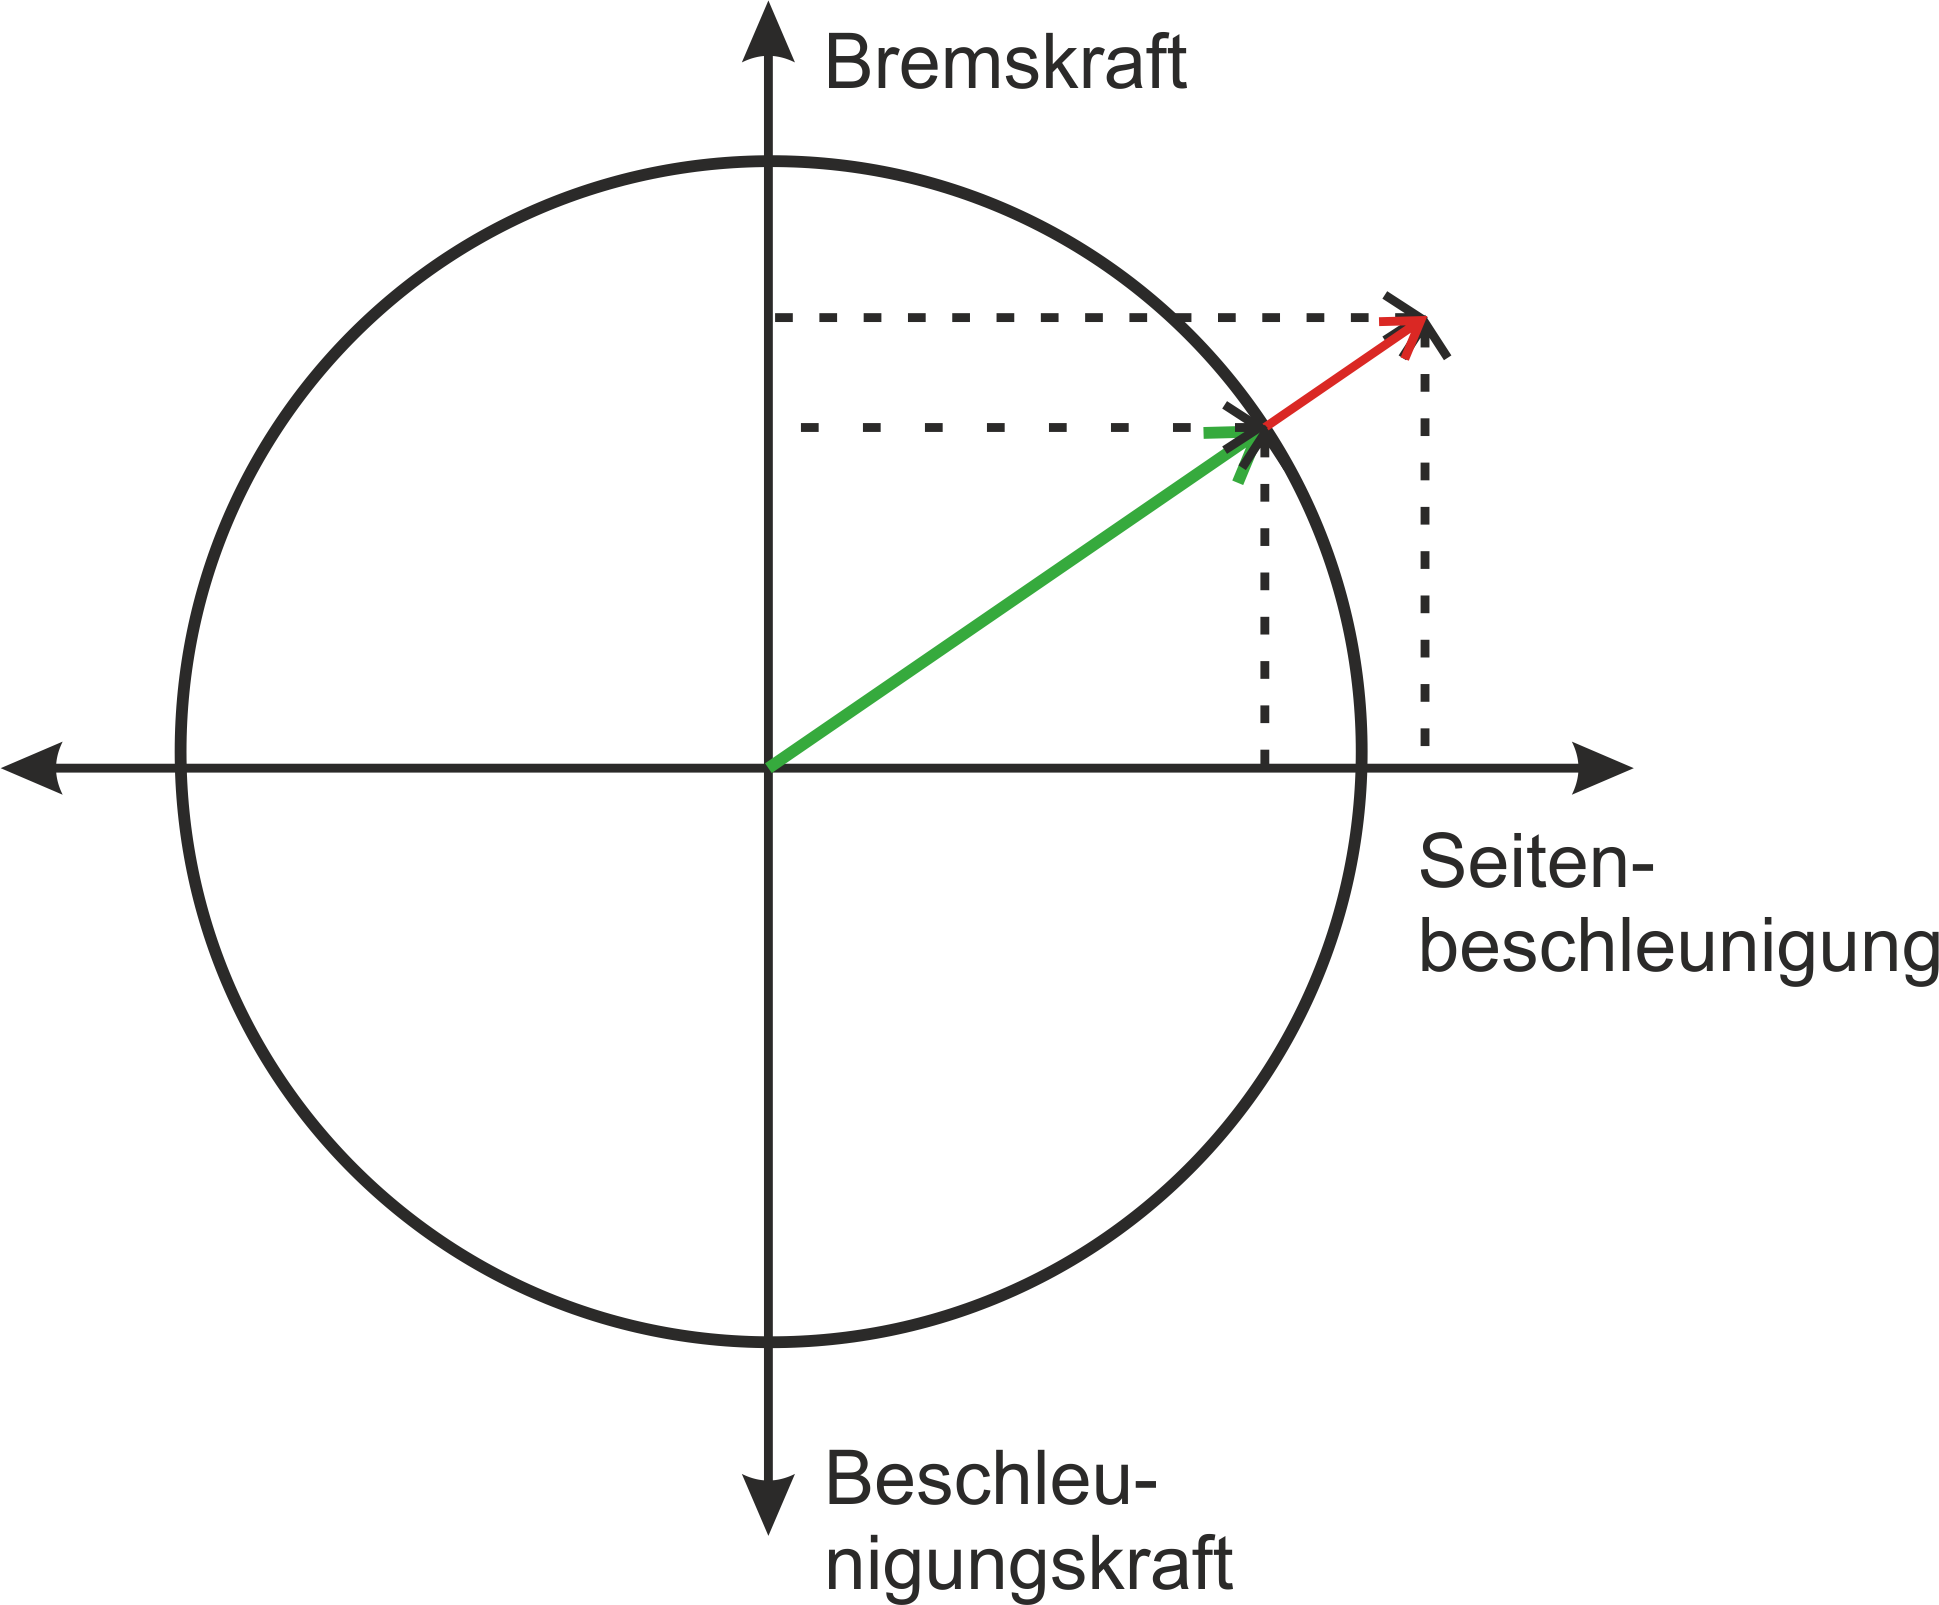
\includegraphics[width=250pt]{Abbildungen/kamKreis.png}
	\caption{Kammscher Kreis: Beschränkung der maximal wirkenden Kraft.}
	\label{fig:kamKreis}
\end{figure}

Dieser schränkt die wirkenden Kräfte so ein, dass die Hypotenuse aus \(F_x\) und \(F_y\) (\ref{maxForceLL}) sich maximal auf einem Einheitskreis bewegen kann (\ref{limitMaxForceLL}). Der Radius entspricht der maximalen Kraft, welche die Reifen übertragen können (\(F_{max}\)).

\begin{eqnarray}
F_{ll} = \sqrt{F_x^2 + F_y^2} \label{maxForceLL} \\
F_{ll} \leq F_{max}  \label{limitMaxForceLL}
\end{eqnarray}
Falls die Kraft $F_{ll}$ größer als $F_{max}$ ist, wird das Verhältnis der Kräfte 

\begin{equation}
	\alpha = \arctan(F_x, F_y)
\end{equation}
berechnet und auf $F_{max}$ 
\begin{eqnarray}
F_x = F_{max} \sin(\alpha)\\
F_y = F_{max} \cos(\alpha)
\end{eqnarray}
herunterskaliert.


Bei einem gleichen Anteil an longitudinaler und lateraler Kraft können die Reifen also das größte Moment auf die Straße übertragen. Dieser Punkt wird von Rennfahrern versucht, in Kurven zu treffen, um das gesamte Potenzial der Reifen auszunutzen.

Mit dem Wissen wie die longitudinalen und lateralen Kräfte berechnet werden, kann nun ein genaueres Systemmodell genutzt werden.

\subsection{Dynamisches Fahrzeugmodell}
\label{dynModel}

Die Basis ist, wie auch schon beim kinematischen Modell, das bicycle model. Es wird nun um die durch das zweite Newtonsche Gesetz entstehenden Kräfte entlang der \(y\)-Achse erweitert.

\begin{equation}
ma_y = F_{yf} + F_{yr}
\end{equation}   


Wobei \(a_y\) aus zwei Anteilen besteht, der Querbeschleunigung \(\ddot{y}\) und der Zentripetalkraft \(\dot{x} \dot{\psi}\).  
Die Kräfte \(F_{yf}\) und \(F_{yr}\) greifen jeweils am vorderen \((.)_f\) und hinteren \((.)_r\) Rad an. Die Zusammenhänge sind im Schaubild \ref{fig:dynModel} veranschaulicht. 

\begin{figure}[ht!]
	\centering
	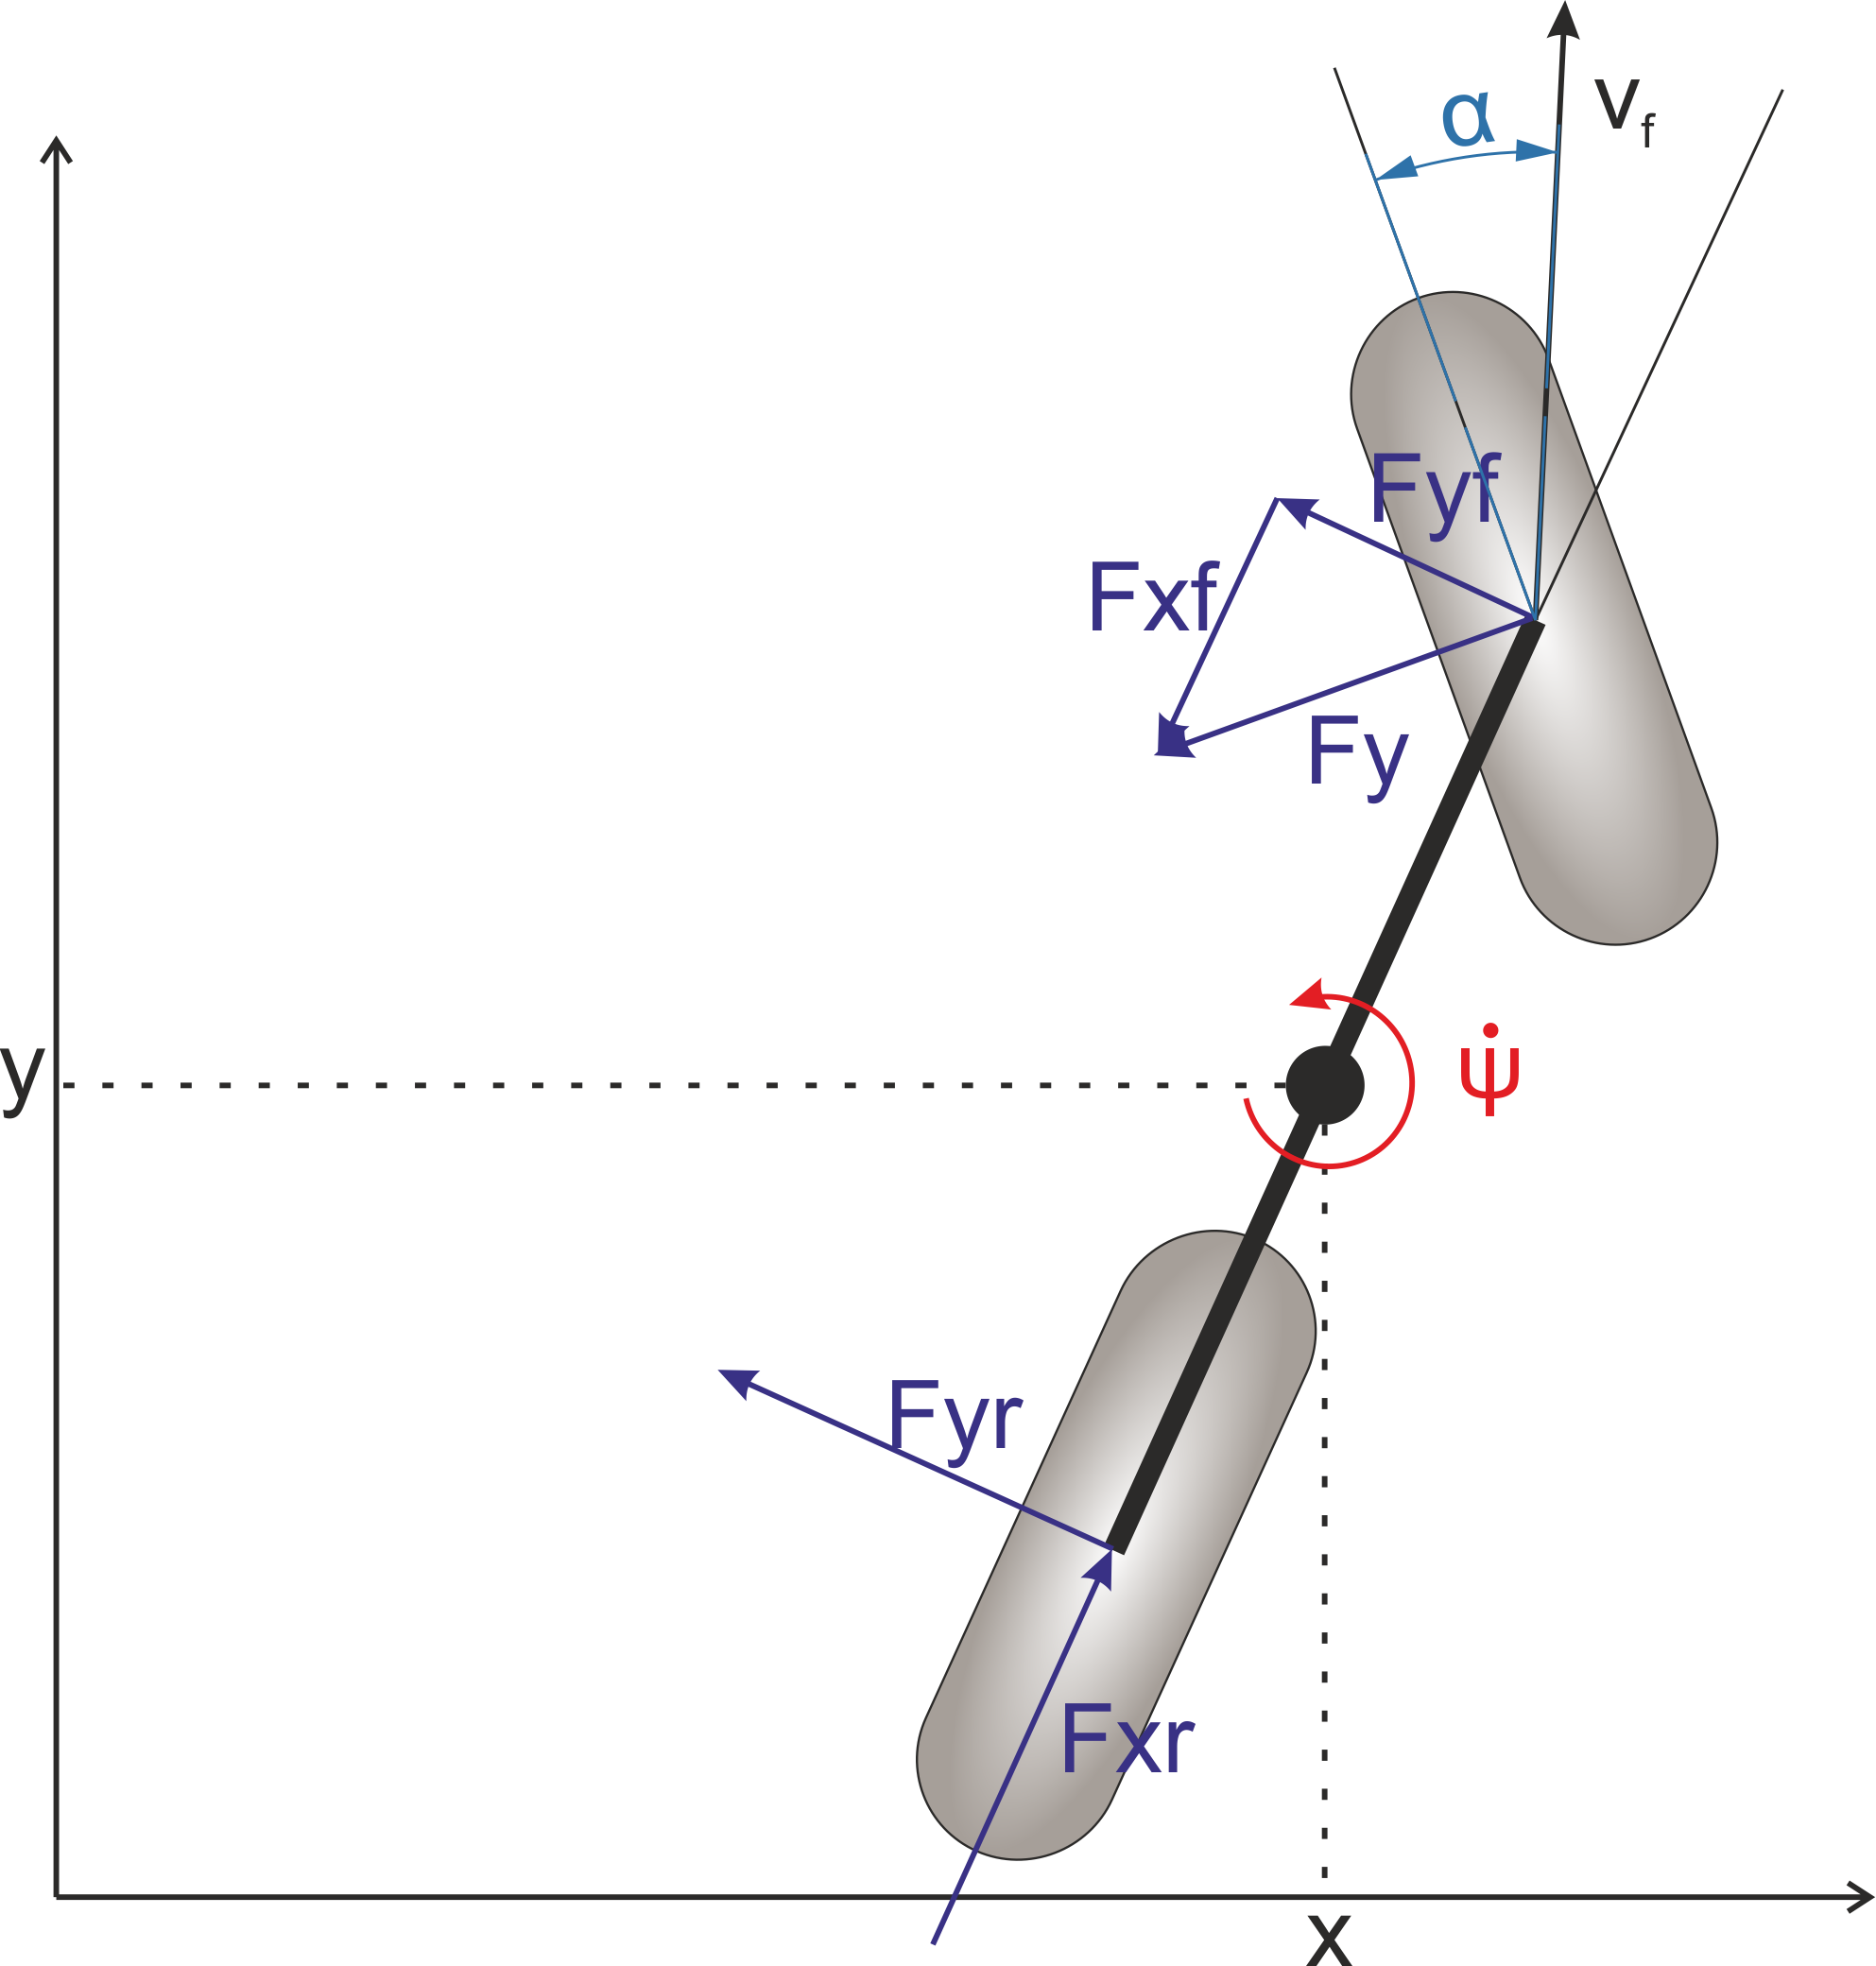
\includegraphics[width=300pt]{Abbildungen/dynBicycle.png}
	\caption{Dynamic Vehicle Model}
	\label{fig:dynModel}
\end{figure}

Unter Berücksichtigung des Trägheitsmoments \(I_z\) des Fahrzeugs, kann das Drehmoment um die \(z\)-Achse betrachtet werden.
\begin{equation}
I_z \ddot{\psi} = l_f F_{yf} - l_r F_{yr}
\end{equation}

Als Ergebnis lassen sich die Gleichungen für die Longitudinal-, Lateral- und Drehbewegung aufstellen.

\begin{eqnarray}
m \ddot{x} = m \dot{y} \dot{\psi} + F_x \\
m \ddot{y} = - m \dot{x} \dot{\psi} + F_y \\
I \ddot{(\psi)} = l_f F_{yf} - l_r F_{yr}
\end{eqnarray}

Die Kräfte \(F_{x}\) und \(F_{y}\) wirken auf den Schwerpunkt des Fahrzeugs und setzen sich aus den Einzelkomponenten der Radkräfte zusammen.

\begin{eqnarray}
F_x = F_{xf} + F_{xr} \\
F_y = F_{yf} + F_{yr}
\end{eqnarray}

Diese hängen ab von den lateralen \((.)_C\) und longitudinalen \((.)_l\)    Radkräften und dem Lenkwinkel. Da das Vorderrad nicht angetrieben wird, besitzt es keinen longitudinalen Anteil. Aus den vom Reifenmodell errechneten Reifenkräften können die resultierenden Kräfte im dynamischen Modell abhängig von dem Lenkwinkel berechnet werden.

\begin{eqnarray}
F_{xf} =& - 2 F_{Cf} \sin(\delta_f) \\
F_{yf} =& 2 F_{Cf} \cos(\delta_f) \\
F_{xr} =&   F_{lr} \\
F_{yr} =& 2 F_{Cr}
\end{eqnarray}
Es ist zu beachten, dass das Fahrzeug in der Realität an jeder Achse zwei Reifen besitzt und daher die Kräfte verdoppelt werden müssen.


Die Kräfte \(F_{Cf}\) und \(F_{Cr}\) werden durch die \ac{M.F.} wie im letzten Abschnitt \ref{tireModel} berechnet.
Die dafür benötigten Schräglaufwinkel werden durch folgende Formeln bestimmt:

\begin{eqnarray}
\alpha_f = \delta_f - \arctan \left(\frac{\dot{y} + l_f \dot{\psi}}{\dot{x}} \right) \\
\alpha_r = - \arctan \left(\frac{\dot{y} - l_r \dot{\psi}}{\dot{x}} \right)
\end{eqnarray}

\subsection*{Longitudinale Kräfte}
Da keine Simulation des Motors genutzt wird, müssen die Kräfte \(F_{lr}\), welche die Reifen longitudinal auf die Straße bringen, anders als über den Schlupf berechnet werden.
Die longitudinale Kraft für Beschleunigung \((.)_{acc}\) und Bremsvorgang \((.)_{dec}\) wird unterschiedlich berechnet. Die Kraft, die der Motor beim Beschleunigen über die Achse an die Reifen übertragt
\begin{equation}
	F_{lr_{acc}} = \frac{P_{engine}}{|\dot{x}|} \label{long_dyn_engine}
\end{equation}
hängt von der Motorleistung $P_{engine}$ und der Geschwindigkeit $\dot{x}$ ab. Die Motorleistung wird über die Gaspedalstellung tp variiert und berechnet sich aus die Gleichung 
\begin{equation}
P_{engine} = P_{engine_{max}} \cdot tp.
\end{equation}
Für kleine Geschwindigkeiten begrenzen die Reifen die maximale auf die Straße übertragene longitudinal wirkende Kraft 

\begin{equation}
	F_{lr_{acc}}\leq 2 F_{max} \label{long_dyn_max}.
\end{equation}

Beim Bremsvorgang, ergibt sich die longitudinale Kraft aus der Bremspedalstellung und den maximalen Reifenkräften.
\begin{equation}
F_{lr_{dec}} = - 2 F_{max} \cdot break
\end{equation} 

Solange sich das Fahrzeug vorwärts bewegt, wirken zusätzlich die Luft- und Rollreibung 
\begin{eqnarray}
F_{roll} = m \mu g \\
F_{aero} = \frac{1}{2} \rho C_d A_f \dot{x}^2
\end{eqnarray}
der longitudinalen Kraft des Motors entgegen.
Diese Gleichungen sind nur zulässig, solange von einem Rennkurs ohne Steigung ausgegangen wird. Die resultierende longitudinale Kraft 
\begin{equation}
F_{lr} = F_{lr} - F_{aero} - F_{roll}
\end{equation}

wird mit der lateralen Kraft im \ac{K.K.} verrechnet und in der finalen Bewegungsgleichung verwendet.

\begin{eqnarray}
\dot{x} =& \dot{x} \cos(\psi) - \dot{y} \sin(\psi) \\
\dot{y} =& \dot{x} \sin(\psi) - \dot{y} \cos(\psi) \\
m \ddot{x} =& m \dot{y} \dot{\psi} + F_{xf} +  F_{xr}\\
m \ddot{y} =& - m \dot{x} \dot{\psi} +  F_{yf} +  F_{yr} \\
I \ddot{\psi} =&  l_f F_{yf} -  l_r F_{yr} 
\end{eqnarray}

Das Gleichungssystem wird hier in diskreter Form dargestellt.

\begin{eqnarray}
x_{k+1} =& X_k + \Delta t(\dot{x}_k \cos(\Psi_k) - \dot{y}_k \sin(\Psi_k) \\
y_{k+1} =& Y_{k} + \Delta t(\dot{x}_k \sin(\Psi_k) - \dot{y}_k \cos(\Psi_k) \\
\Psi_{k+1} =& \Psi_k + \Delta t \dot{\psi}_k \\
\dot{x}_{k+1} =&  \dot{x}_k + \Delta t \left(\frac{F_{xf_k} +  F_{xr_k}- F_a}{m} + \dot{y}_k \dot{\psi}_k \right) \\
\dot{y}_{k+1} =&  \dot{y}_k + \Delta t \left(\frac{ F_{yf_k} +  F_{yr_k}}{m} - \dot{x}_k \dot{\psi}_k \right)  \\
\dot{\psi}_{k+1} =& \dot{\psi}_k + \Delta t \left( \frac{ l_f F_{yf} -  l_r F_{yr}}{I}  \right)\\
\end{eqnarray}

Im dynamischen Fahrzeugmodell ändert sich damit auch der Zustandsvektor \\
\(x\), \(y\), \(x_d\), \(y_d\), \(\Psi\), \(\dot{\psi}\). \\

Die Fahrzeugparameter \ref{vehicleParam} die zur Berechnung verwendet wurden, beziehen sich auf das aktuellste Fahrzeug des High-Octane Motorsports Verein.

\begin{table}[]
	\centering
	\caption{Fahrzeug Parameter}
	\begin{tabular}{l|l|l}
		\hline
		Formelzeichen	& Wert & Einheit \\ \hline
		\(l_f\)	&	0,66 & m\\
		\(l_r\)	&	0,97 & m\\
		\(l_b\)	&	1,53 & m \\
		\(r\)	&	0,2 & m \\
		\(m\)	&  	220 & kg\\
		\(I\)	&  	400 & kgm\textsuperscript{2}\\
		\(A_f\)	&  	0,6 & m\textsuperscript{2}\\
		\(P_{engine}\) &  53 & kW\\
		\(C_d\)	&  	1.5 & - \\
		\(\rho\)	&  	1,225 & $\frac{\text{kg}}{\text{m\textsuperscript{3}}}$\\
		\(F_{max}\)	&  	1,6 & kN \\ 
	\end{tabular}
	\label{vehicleParam}
\end{table}



\chapter{MPC zur Trajektorienplanung und Regelung}

Ein schneller Rennfahrer zeichnet sich dadurch aus, dass er genau abschätzen kann, wie viel Kräfte die Reifen des Fahrzeugs auf die Straße übertragen können. Die Kunst liegt also darin, möglichst in jeder Fahrsituation das gesamte Potential voll auszunutzen. Zudem kann er sich dynamisch an Änderungen der Streckenverhältnisse anpassen und versucht immer die Idealtrajektorie zu treffen. Die Definition dieser ist die größtmögliche Streckenlänge in kleinstmöglicher Zeit zurückzulegen. Für eine Gerade oder eine einzige Kurve ist dies in Abbildung \ref{fig:idealTrajektorie} dargestellt. Der sogenannte Scheitelpunkt markiert hierbei den Punkt des geringsten Radius und der kleinsten Geschwindigkeit. An diesem Punkt muss das Fahrzeug im besten Fall genau die Seitenbegrenzung tangieren. 
Bei komplexeren Streckengefügen kann es jedoch von Vorteil sein, eine Kurve eventuell nicht ideal auszufahren, um im späteren Verlauf einen größeren Geschwindigkeitsgewinn in einer anderen Kurve einfahren zu können.

\begin{figure}[ht!]
	\centering
	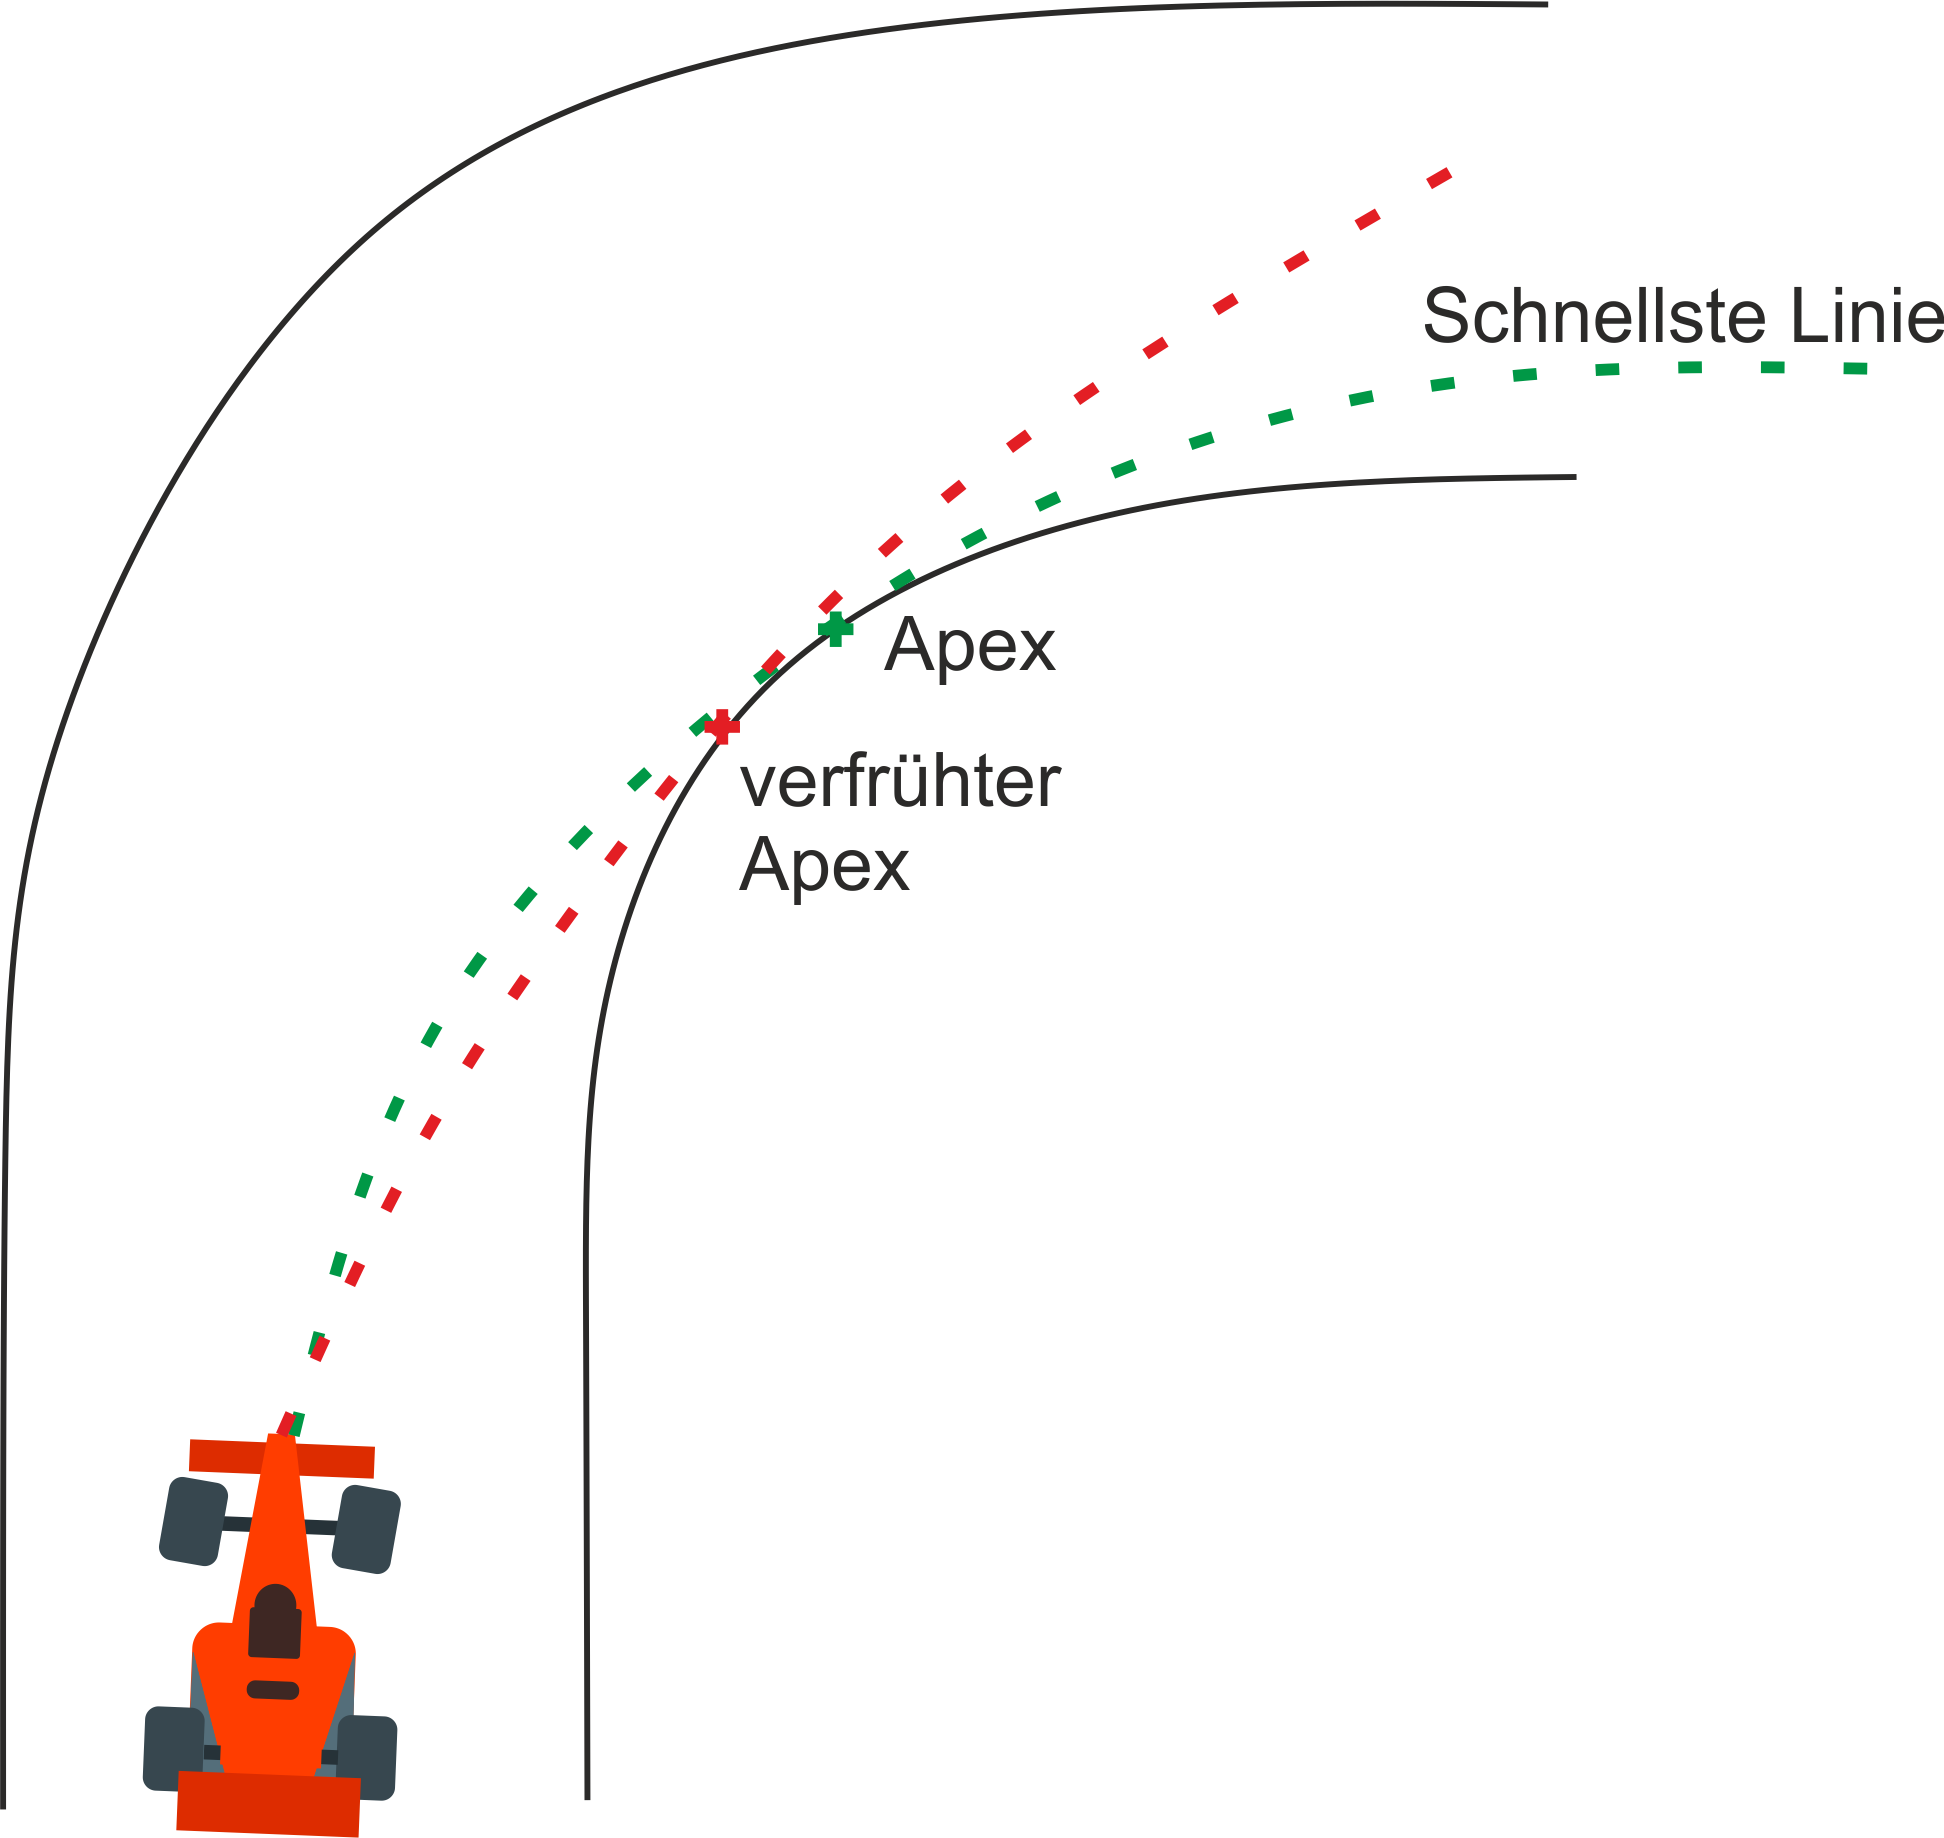
\includegraphics[width=250pt]{Abbildungen/apexTrajektory.png}
	\caption{Ideale Trajektorie für eine 90 Grad Kurve}
	\label{fig:idealTrajektorie}
\end{figure}


Um all dies mit dem \ac{MPC}-Algorithmus nachzustellen, wird im Folgenden auf die einzelnen Schritte bei der Entwicklung eingegangen.

Zu Beginn hätte die Möglichkeit bestanden die Regelung der lateralen und longitudinalen Führung des Fahrzeuges zu trennen. 
Vorteile hierfür wären gewesen:
\begin{itemize}
	\item Einfachere Anpassung der Parameter für das reale Fahrzeug
	\item Robustheit. Der Ausfall eines Reglers würde zumindest noch eine eingeschränkte Kontrolle ermöglichen
	\item Zwei einfacher zu berechnende Probleme. Da die Berechnungszeit nicht linear mit der Komplexität steigt, wären hier möglicherweise deutliche Geschwindigkeitssteigerungen möglich
	\item Ein weniger komplexer \ac{MPC}-Ansatz ist einfacher zu testen und zu entwickeln
\end{itemize}

Die Vorteile werden aber mit dem Nachteil begleitet, dass bei einem Rennauto die longitudinale und laterale Bewegung des Fahrzeugs stark miteinander korrelieren. Durch die Trennung kann keine optimale Lösung mehr gefunden werden. 
Zudem ist die Integration komplexer, da beide Regler gleichzeitig laufen und ihre Berechnungen miteinander ausgetauscht werden müssen.
Aufgrund des Anwendungsszenarios wurde sich gegen den zweigeteilten Ansatz entschieden.


Der erste Schritt ist das Erstellen des Vektors an Einflussparametern $\vec{X}$. Er setzt sich immer aus der Kombination von Systemzustand und Steuerparametern zusammen  $\vec{x} = [x, y, v, \psi, a, \delta ]^T $ (siehe \ref{kinematicModel}). 
Dieser Teilvektor wird dann für die Anzahl der gewünschten Prädiktionsschritte \(N\) mal in $\vec{X}$ wiederholt. 
Da zusätzlich zu den Prädiktionsschritten auch der aktuelle Fahrzeugzustand benötigt wird, besteht der Vektor also aus $N+1$ Teilvektoren $\vec{x}$. In Vektordarstellung entspricht dies dann: \\
$
\vec{X} = 
\begin{bmatrix}
\vec{x_0} \\ \vec{x_1} \\ . \\ . \\ \vec{x_N}
\end{bmatrix}
$ mit  $ \vec{x_i} = \begin{bmatrix}
x_i \\ y_i \\ v_i \\ \psi_i \\ a_i \\ \delta_i 
\end{bmatrix} $

 In der Abbildung \ref{fig:predictionMpc} ist grafisch dargestellt, wie die Prädiktion für $N=3$ ausschaut.
\begin{figure}[ht!]
	\centering
	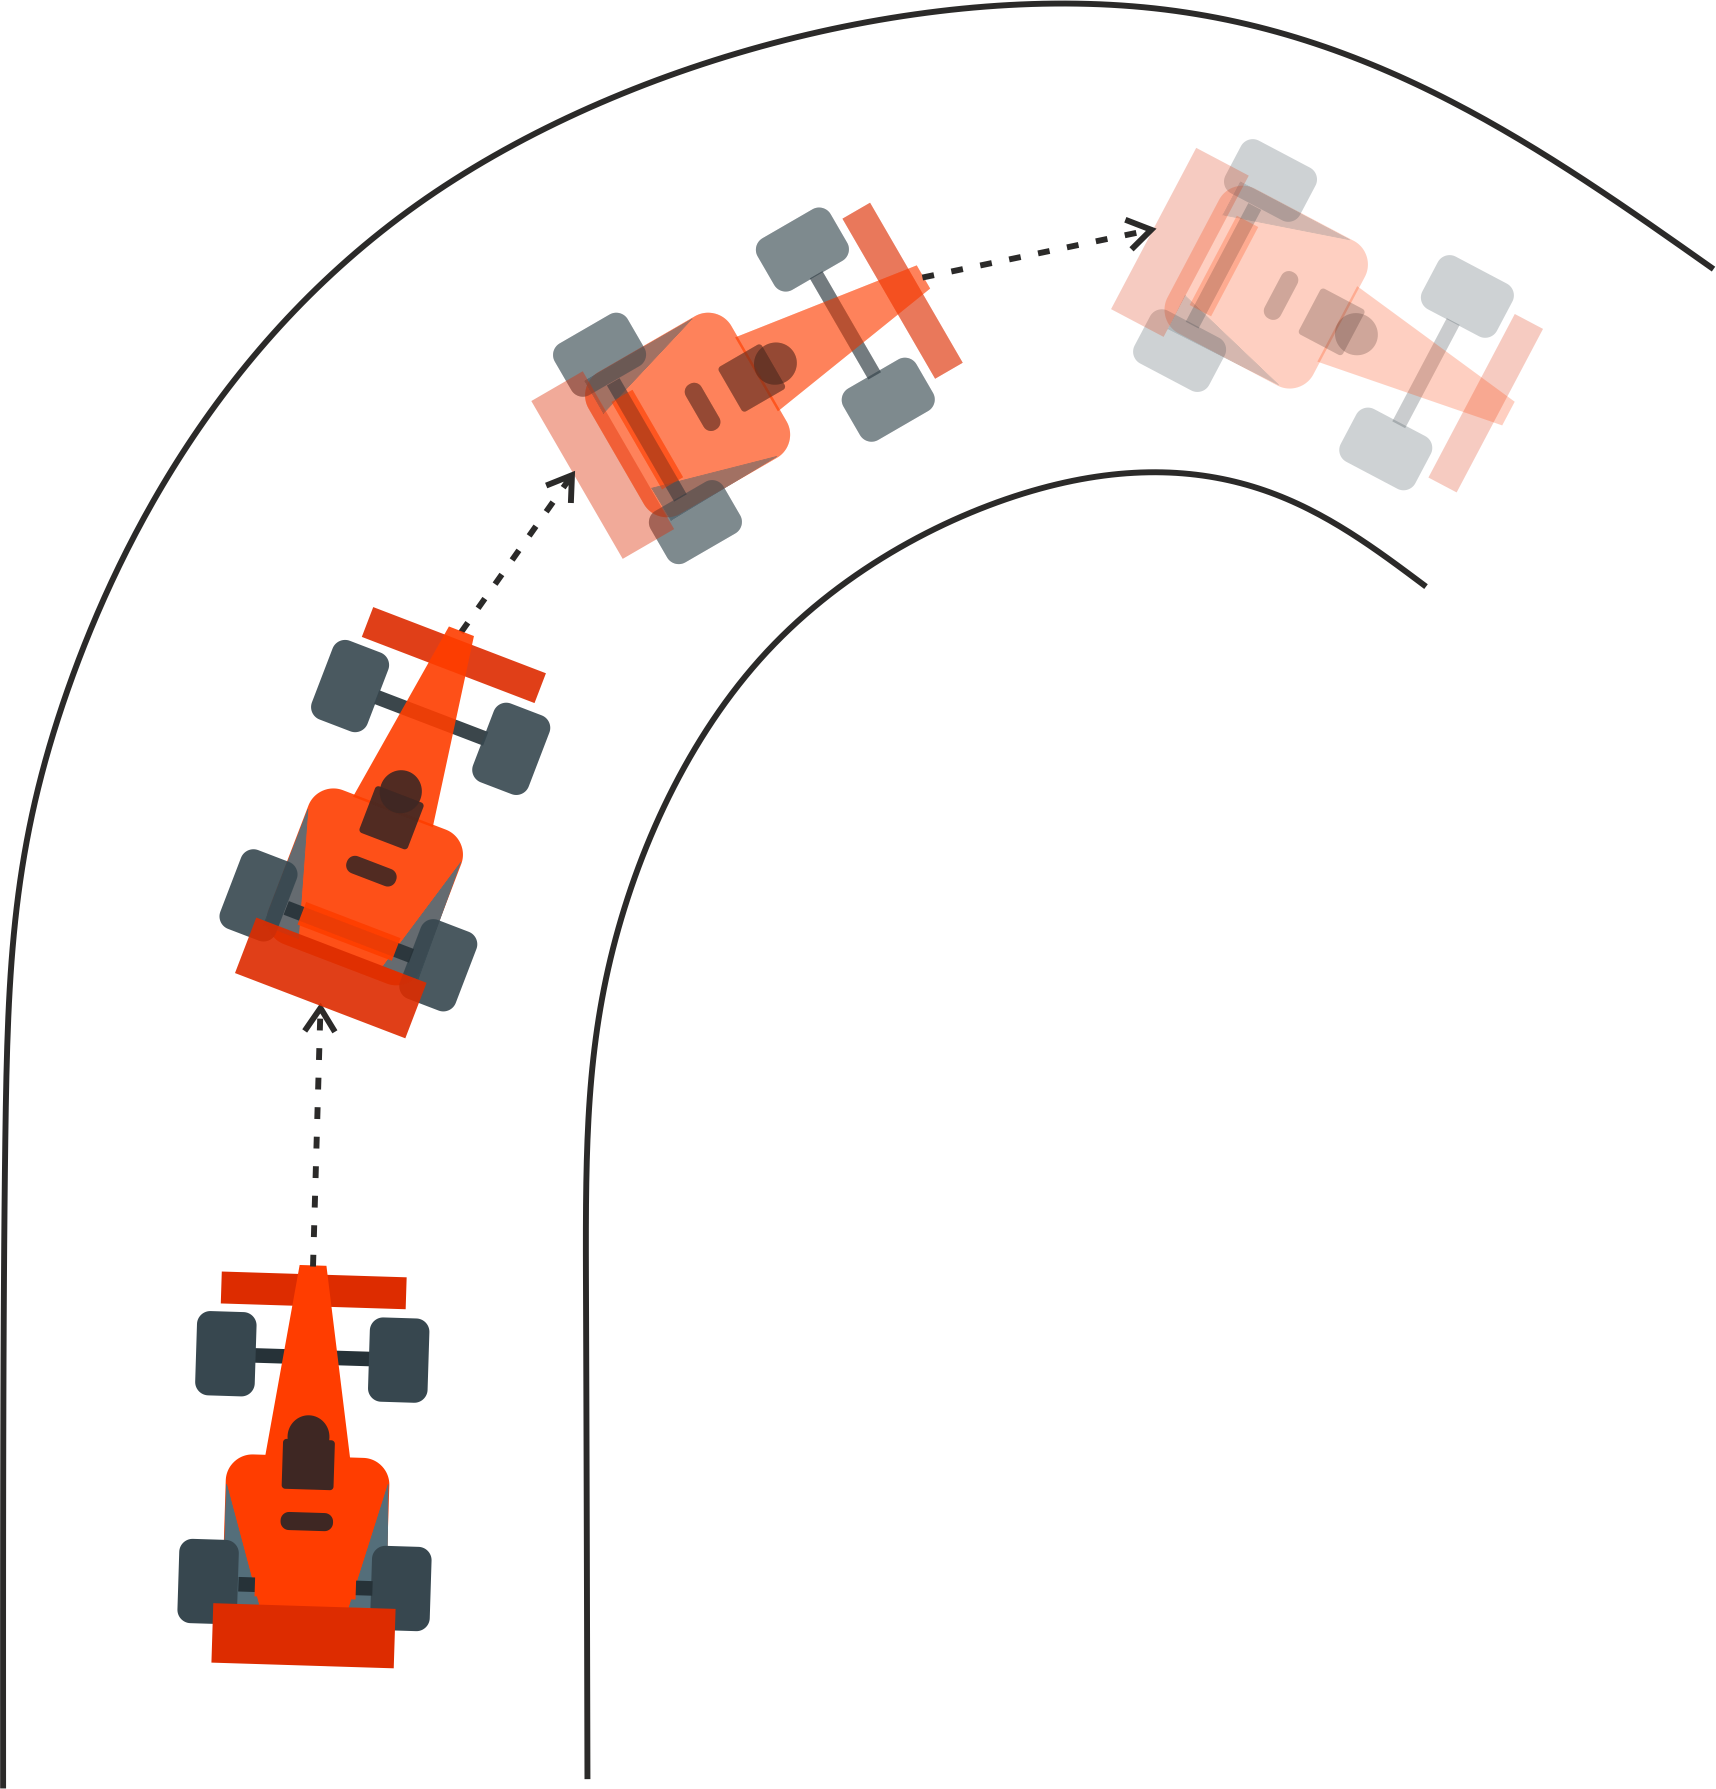
\includegraphics[width=150pt]{Abbildungen/predictionMPC.png}
	\caption{Grafische Visualisierung der Prädiktion abhängig von den Steuerparametern für drei Schritte in die Zukunft}
	\label{fig:predictionMpc}
\end{figure}
Zwischen jedem der einzelnen Schritte wird ein $\Delta t$ angenommen, dass dem der Positionsschätzung entspricht, also $\frac{1}{20}$ s. Obwohl immer nur der erste Steuerbefehl des berechneten Steuervektors im realen System angewandt wird, ist der Vektor trotzdem von Nutzen. Sollte die Optimierung, unterbrochen durch andere Prozesse, einmal nicht schnell genug sein, können die Steuerbefehle aus der vorherigen Optimierung verwendet werden. Dies funktioniert solange die Zeitverzögerung kleiner als die gesamte Zukunftsprädiktion ist. Obwohl diese Werte zum Regeln genutzt werden können, nimmt aufgrund von Modellfehlern die Güte der berechneten Werte mit der Anzahl der Prädiktionsschritte ab. Es ist also nicht sinnvoll, den \ac{MPC}-Algorithmus langsamer als die Positionsschätzung berechnen zu lassen. 

  

Nachdem der Vektor mit den Einflussparametern definiert ist, werden im nächsten Schritt alle Beschränkungen sukzessive ergänzt.

\section{Fahrzeugmodell}
Zu Beginn haben die Teilvektoren $\vec{x}$ keinen Bezug zueinander. Da jedoch die einzelnen Prädiktionsschritte voneinander über den Fahrzeugzustand, Steuerparameter und das Fahrzeugmodell zusammenhängen, werden im zweiten Schritt die Beschränkungen hierfür definiert und als Ungleicheitsbedingungen in das zu optimierende nichtlineare Problem integriert. Dazu wird die diskretisierte Form des Systemmodells genutzt, um immer zwei aufeinander folgende Schritte miteinander zu verknüpfen. 

Zusätzlich zu der Systembeschreibung fehlen noch Einschränkungen für den Optimierer, welche die physikalischen Eigenschaften des Rennautos abbilden.
Dazu zählen die maximale Geschwindigkeit, Beschleunigung und Lenkwinkel. 
Diese Beschränkungen werden für jeden der Teilvektoren hinterlegt. 
Zusammen mit dem Fahrzeugmodell benötigt das \ac{MPC} noch eine Kostenfunktion, damit der Optimierer überhaupt einen Anlass hat das Rennauto zu Beschleunigen.


\section{Kostenfunktionen}
\label{costFunctions}
Erst eine geeignete Kostenfunktion führt zu der Planung einer Trajektorie, die das Rennauto um den Kurs führt. Es wurden drei verschiedene Kostenfunktionen implementiert:

\subsubsection*{Maximalgeschwindigkeit}  
Mit der Funktion 
\begin{equation}
	f(\vec{X}) =  \sum_{1}^{N} \frac{1}{v_i}
\end{equation}
wird die Summe aller inversen Geschwindigkeitswerte der einzelnen Prädiktionsschritte addiert und als Kosten versucht zu maximieren.
Die Berechnung bezieht den Geschwindigkeitswert aus dem aktuellen (0-ten) Fahrzeugzustand nicht ein, da der Optimierer keinen Einfluss mehr auf diesen hat. Der Vorteil dieser Funktion ist die einfache Berechnung und leichte Integration in den \ac{MPC}-Algorithmus. Im weiteren Verlauf wird diese Kostenfunktion als max-speed bezeichnet.

\subsubsection*{Zielpunkt Distanzminimierung}
Für diese Kostenfunktion wird vor dem letzten Prädiktionsschritt ein virtuelles Ziel definiert und die Distanz des $N+1$ Schrittes zu diesem Ziel minimiert. Der Optimierer wird also Steuerparameter suchen, die ihn möglichst dicht an dieses Ziel bringen. Das virtuelle Ziel wird nach jedem Update wieder so neu positioniert, dass das Rennauto den Punkt niemals erreichen kann und damit konstant schnell weiterfährt. Die Distanz $d_{goal}$, in der das virtuelle Ziel platziert wird, errechnet sich durch die maximale Geschwindigkeit und die Anzahl der Prädiktionsschritte durch die Gleichung 
\begin{equation}
d_{goal} = \left(v_0 + N \cdot v_{max} \right) \Delta t.
\end{equation}


Eine bildliche Darstellung der Kostenfunktion ist in Abbildung \ref{fig:costGoalDist} zu sehen. 

\begin{figure}[ht!]
	\centering
	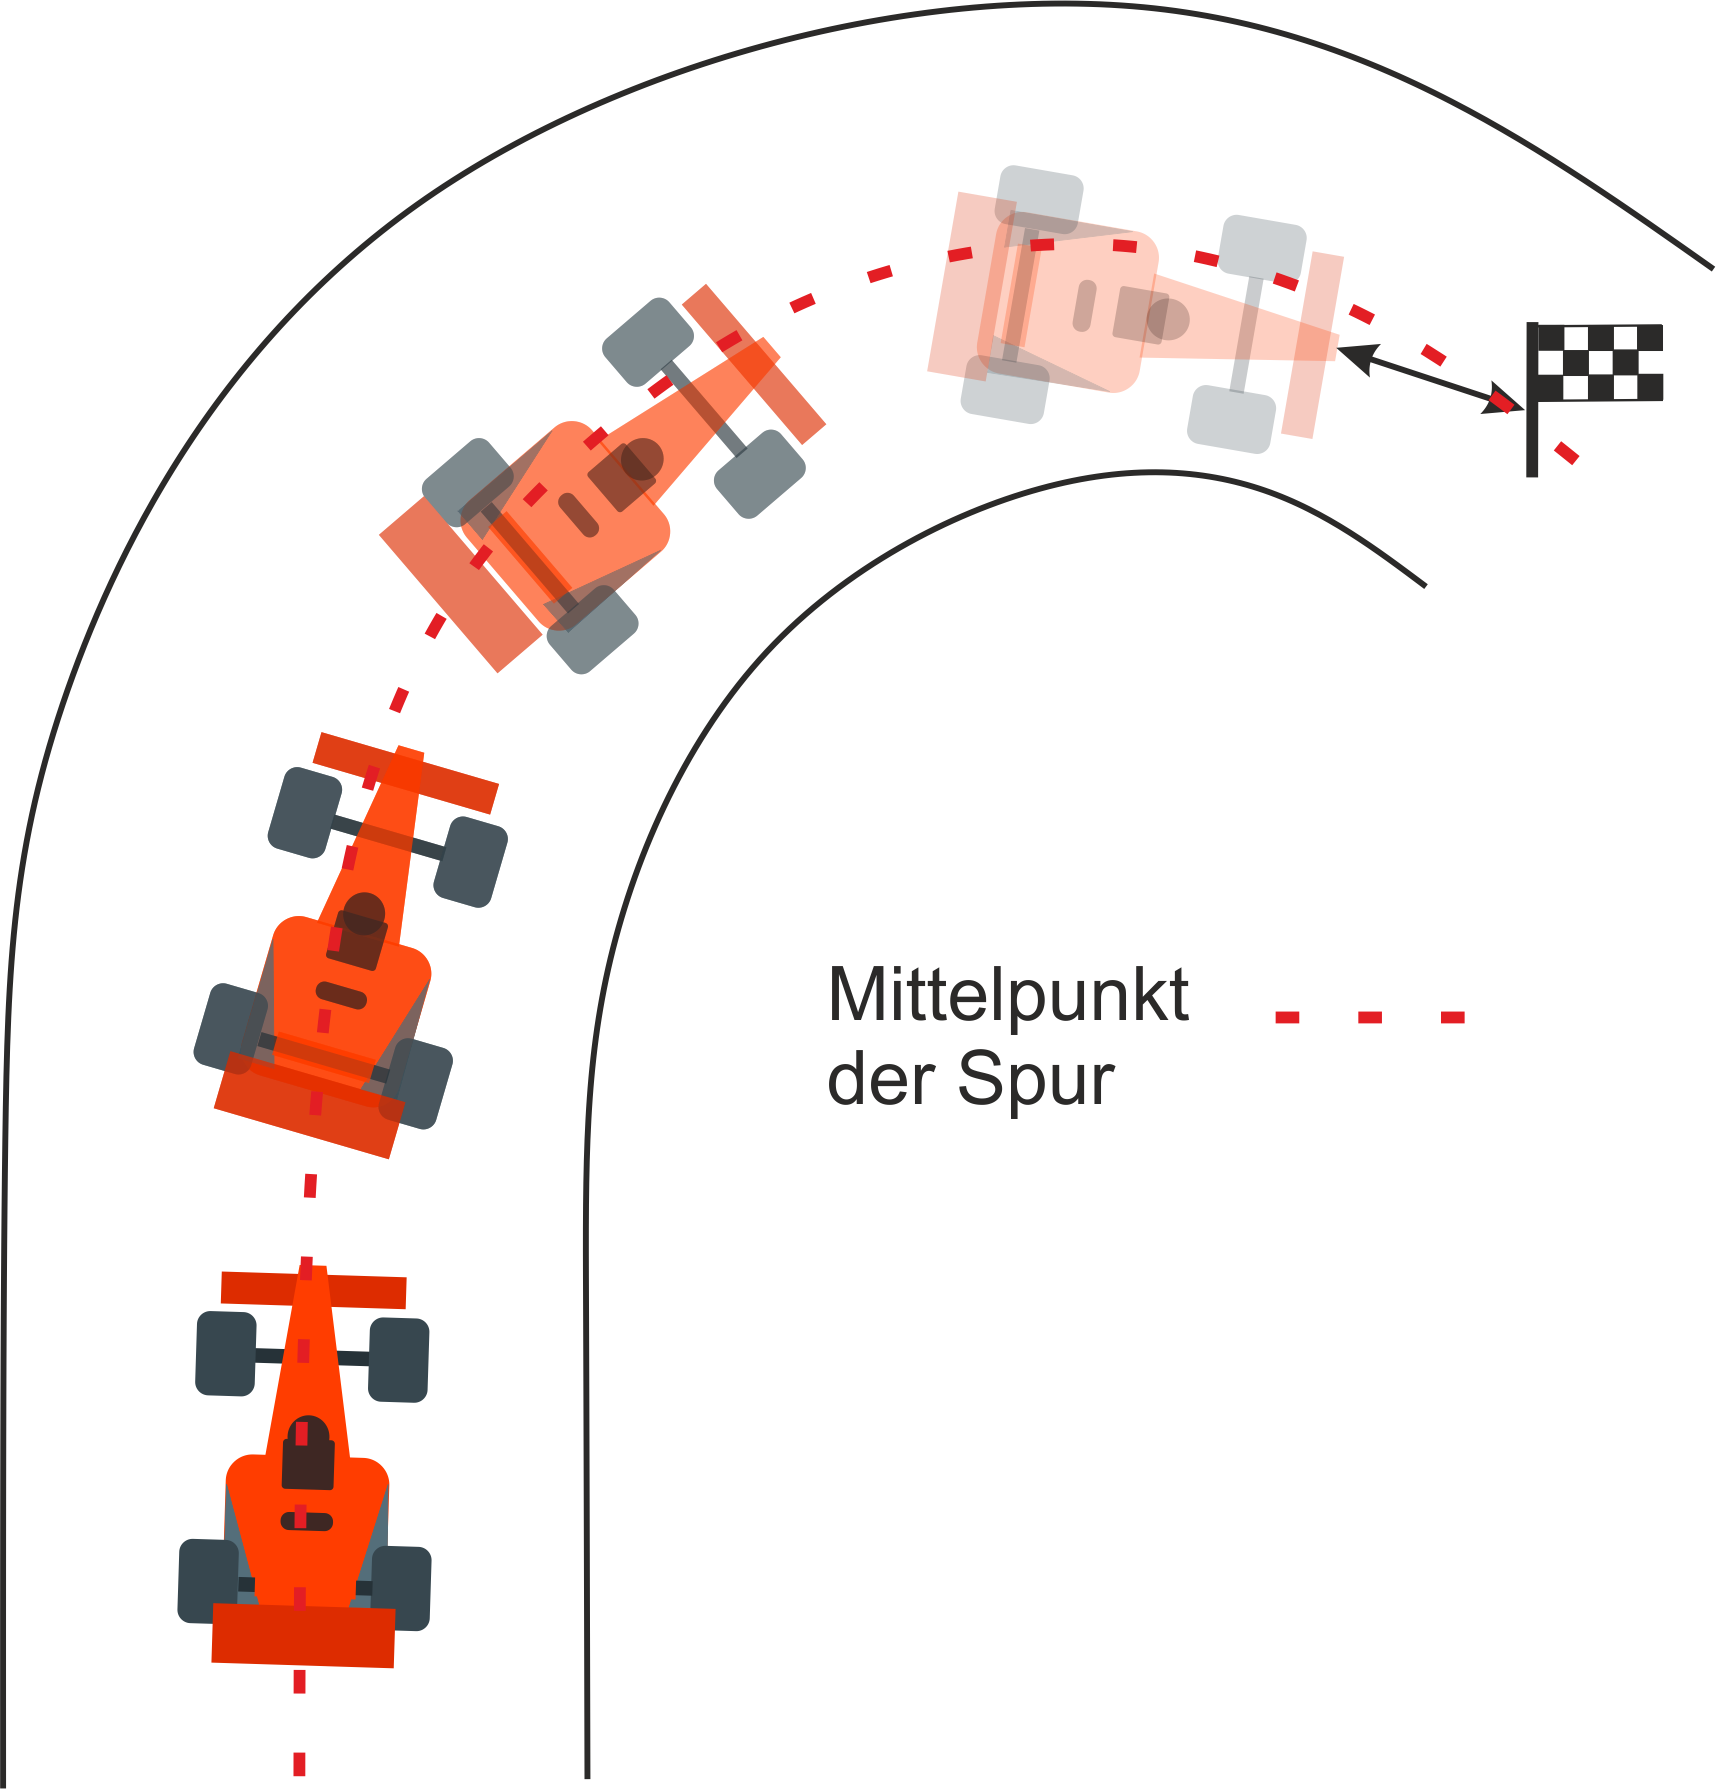
\includegraphics[width=200pt]{Abbildungen/costGoalDist.png}
	\caption{Zielpunkt Distanzminimierung: Das virtuelle Ziel wird immer weit genug vor dem Fahrzeug hergeschoben, so dass es nie erreicht werden kann}
	\label{fig:costGoalDist}
\end{figure}
Im weiteren Verlauf wird diese Kostenfunktion mit min-dist bezeichnet.

\subsubsection*{Maximieren der Streckendistanz}
Um eine Kostenfunktion zu finden, die einer Idealtrajektorie am nächsten kommt, muss überlegt werden wie diese gemessen werden kann. Die bestmögliche Trajektorie ist diejenige, welche für ein $\Delta t$ die zurückgelegte Strecke, nicht bezogen auf das Fahrzeug, sondern auf den Rennkurs, maximiert. Würde die vom Rennauto zurückgelegte Strecke maximiert werden, würde das Rennauto einfach immer an der äußeren Begrenzung des Kurses entlang fahren. Die Streckenmaximierung lässt sich zu einer Minimierung der nach einem Zeitschritt übrig bleibenden Reststrecke umformen. Die Reststrecke wird einfachheitshalber auf einen Punkt bezogen, der in einer Distanz vor dem letzten Prädiktionsschritt liegt, den dieser nicht erreichen kann. Der Unterschied zur Kostenfunktion, welche die Distanz minimiert ist, dass sich die Differenz nicht auf einen Punkt, sondern auf eine Gerade senkrecht zur Rennkursmitte bezieht.
Realisiert wird dies durch eine Vektorabbildung (eng.: vector rejection)
\begin{equation}
	d = |a - \frac{ab}{bb}b|.
\end{equation}
Der Vektor vom Mittelpunkt der Strecke zum Massenschwerpunkt des Fahrzeugs wird als a bezeichnet und b als der Vektor vom Mittelpunkt der Strecke zur Streckenbegrenzung.
Der Zusammenhang ist in der Grafik \ref{fig:maxDist} grafisch  veranschaulicht. Zur besseren Darstellung wurde die Nase des Rennautos und nicht der Massenschwerpunkt gewählt.

\begin{figure}[ht!]
	\centering
	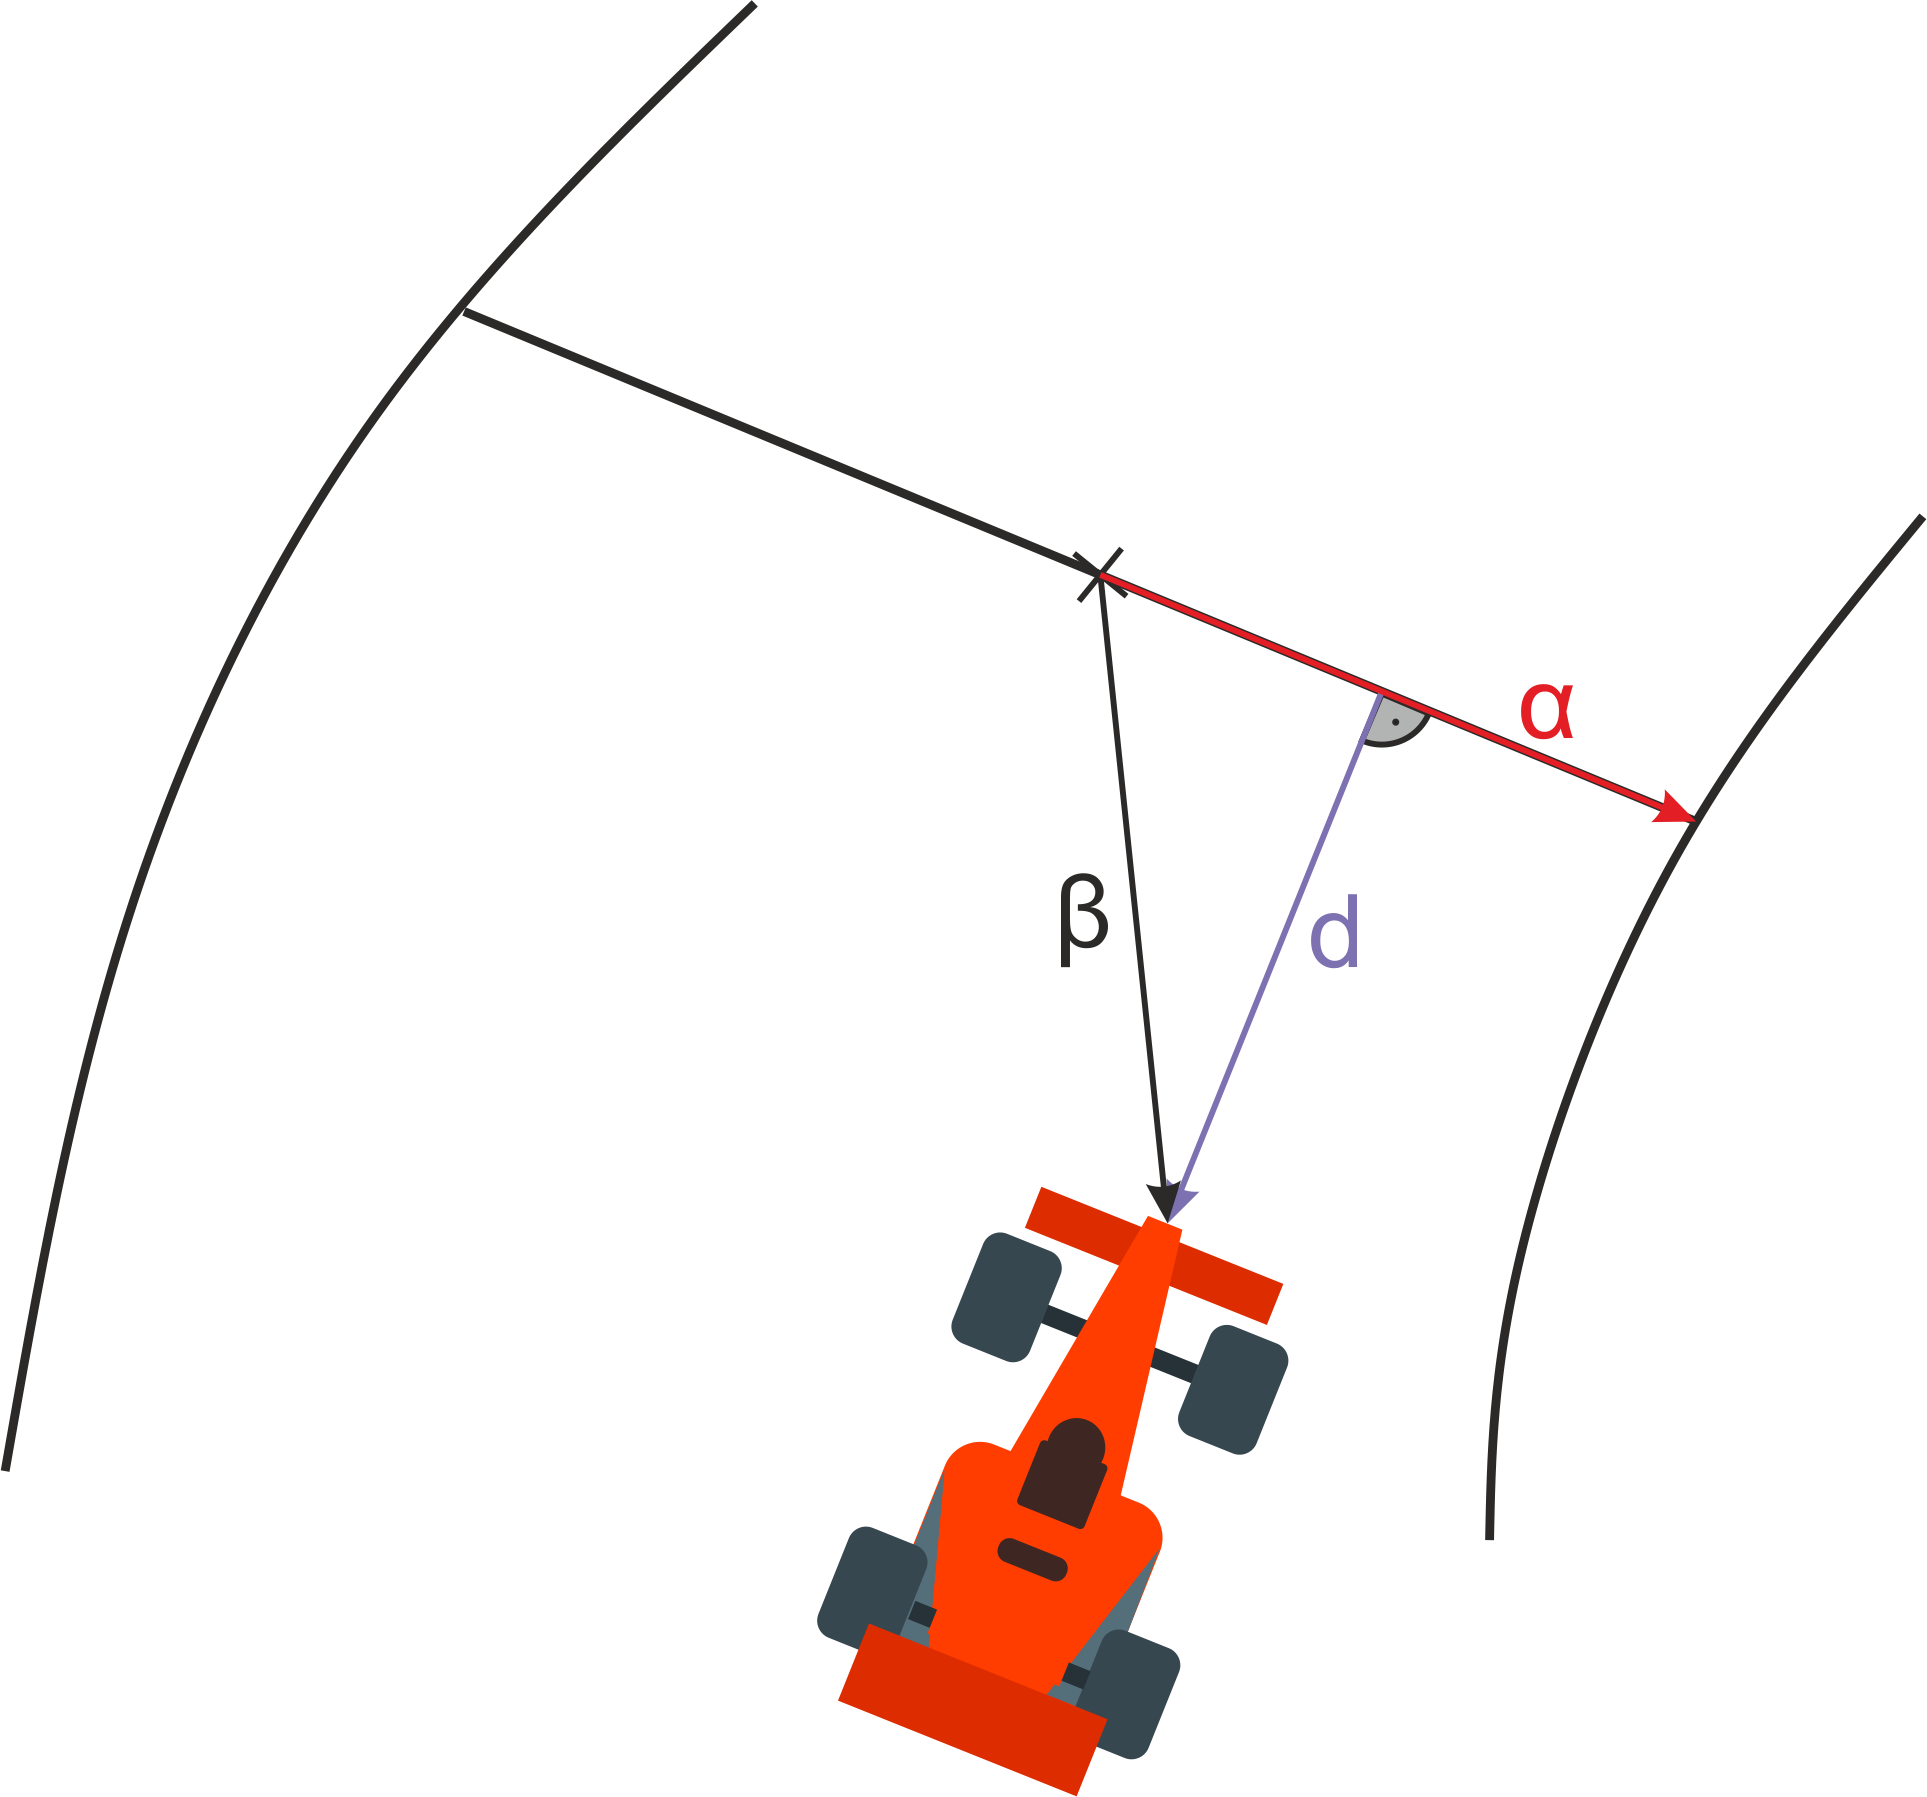
\includegraphics[width=200pt]{Abbildungen/vektorRejection.png}
	\caption{Maximieren der Streckendistanz}
	\label{fig:maxDist}
\end{figure}
Im weiteren Verlauf wird diese Kostenfunktion als max-track bezeichnet.

\section{Strecken-, und Positionsbeschränkung}
\label{trackAndPosConstraint}
In Folge der Kostenfunktionen werden die Steuerparameter durch den Optimierer so angepasst, dass die Kosten minimal werden. Dies würde auf einem Rennkurs zum Abkürzen bei Kurven führen, da in diesem Fall die Kosten geringer werden. Um das zu verhindern, wird eine zusätzliche Streckenbeschränkung eingeführt. Diese basiert auf zwei Tangenten, die für jeden Prädiktionsschritt an die Fahrbahnaußen- und innenseite projiziert werden. Die Tangenten sind in der Abbildung \ref{fig:tangentialConstraint} dargestellt.
\begin{figure}[ht!]
	\centering
	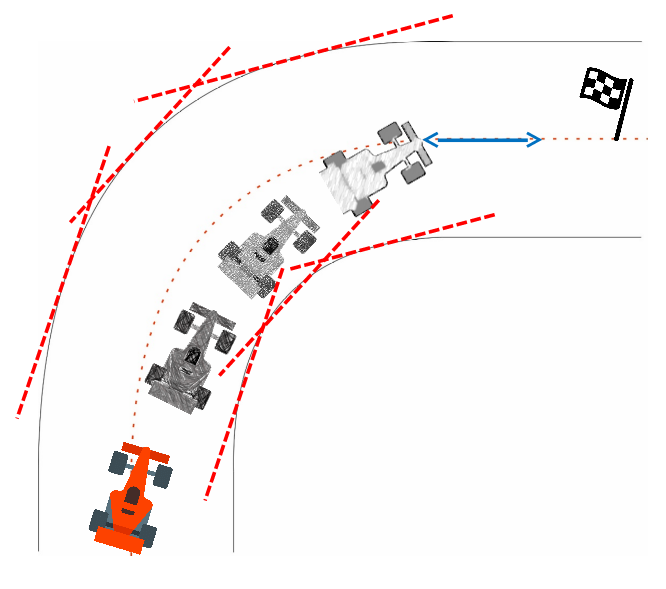
\includegraphics[width=200pt]{Abbildungen/tangentialConstraint.png}
	\caption{Tangentiale Begrenzung hält das Fahrzeug auf der Fahrspur}
	\label{fig:tangentialConstraint}
\end{figure}

Solange sich jeder Prädiktionsschritt innerhalb seines Tangentenpaares bewegt, ist die Beschränkung erfüllt. Während des Optimierungsvorgangs wird die Position der Tangenten nicht verändert. Der Prädiktionsschritt \(n\) benötigt einen passenden Streckenabschnitt, für den die Beschränkungen ausgelegt werden. Dazu kann auf die Ergebnisse der vorausgehenden Optimierung zurückgegriffen werden. Die Position des $n+1$-Schrittes wird gewählt und für diesen die Tangenten berechnet. Für den letzten Schritt \(N +1\) ist dies nicht möglich, hier wird mithilfe der Geschwindigkeit und Orientierung ein virtueller Punkt projiziert.   


Dieses Verfahren funktioniert nur durch die physikalischen Grenzen der Beschleunigung des Rennautos. Das Fahrzeug bewegt sich immer in einem bestimmten Bereich um den Punkt herum, der bei gleichbleibender Geschwindigkeit $\Delta t \cdot v$ Meter entfernt von seinem Vorgängerzustand liegt. Wenn sich dieser Punkt in einer Kurve direkt an der Streckenmarkierung befindet, könnte das Fahrzeug sich vom Kurs herunter bewegen, obwohl die Tangentialbeschränkung erfüllt ist. Dies wird dadurch verhindert, dass der nächste Prädiktionsschritt in diesem Fall seine Beschränkung nicht mehr erfüllen würde.
Mathematisch lassen sich die Tangenten durch eine Vektorprojektion 
\begin{equation}
	d = \frac{a*b}{|b|}
\end{equation}
darstellen. Der Vektor vom Mittelpunkt der Strecke zum Massenschwerpunkt des Rennautos entspricht a und der Vektor vom Mittelpunkt zum Rand des Rennkurses b. Mit der Beschränkung der Distanz $|d|$ auf die Hälfte der Rennkursbreite wird also sichergestellt, dass das Rennauto immer auf dem Kurs bleibt.
Die Vektorprojektion ist im Schaubild \ref{fig:vektorProjektion} dargestellt.

\begin{figure}[ht!]
	\centering
	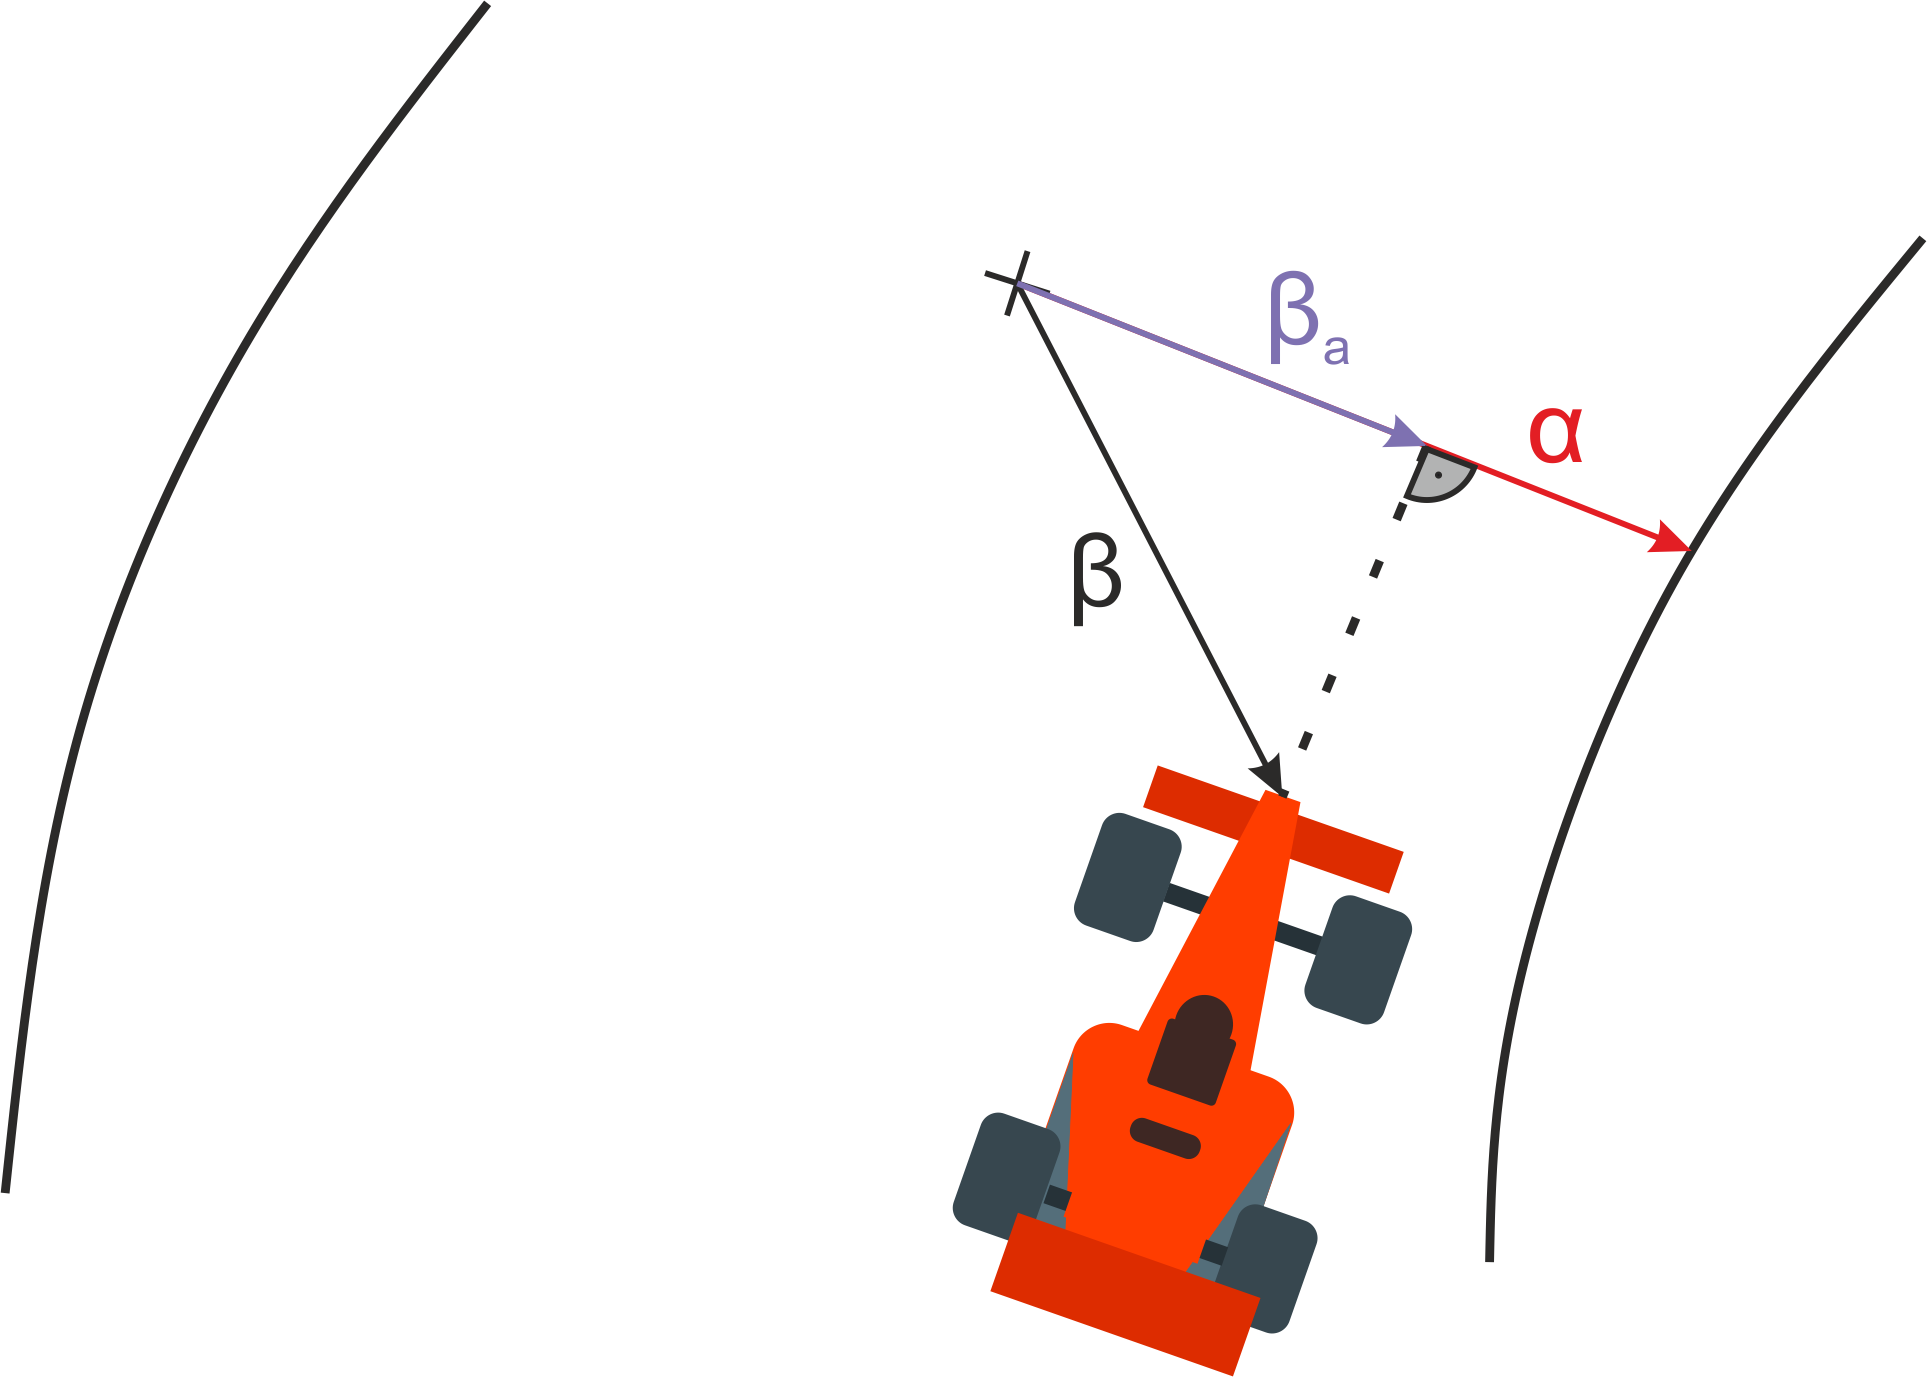
\includegraphics[width=200pt]{Abbildungen/vektorProjection.png}
	\caption{Vektor Projektion zum berechnen der tangentialen Beschränkung}
	\label{fig:vektorProjektion}
\end{figure}

Für diese Beschränkung können sich die Räder des Fahrzeuges über den Rand hinausbewegen. Soll dies verhindert werden, muss diese Beschränkung auf jedes der einzelnen Räder erweitert werden. Das einfache verjüngen der Streckenbreite ist nicht ausreichend, da der Schwerpunkt des Fahrzeugs nicht in der Mitte liegt und das Fahrzeug auch quer stehen kann.

Im letzten Schritt, bevor der \ac{MPC}-Algorithmus funktionsbereit ist, wird der Fahrzeugzustand des aktuellen Zeitschritts $t_0$ als Beschränkung verankert.  Dies ist nötig um zu verhindern, dass der Optimierer einfach die \(x\)-, und \(y\)-Position auf den Punkt legt, welcher die Kostenfunktion ideal minimiert. 

\subsubsection*{Suchbereichsbeschränkung}
Während dem Testen der Kostenfunktion zum Maximieren der Geschwindigkeit ist ein Phänomen aufgetreten. Der Optimierer fand augenscheinlich unmögliche Lösungen, bei denen sich das Rennauto links aus einer Rechtskurve und andersherum herausbewegt.
Dies passiert jedoch nur in Kurven, die mehr als 90° aufweisen. Der Grund hierfür, liegt in den tangentialen Beschränkungen und darin, dass sie immer nur am Anfang des \ac{MPC}-Zyklus aktualisiert werden. Werden die Tangenten wie in Abbildung \ref{fig:curveAnomaly} sehr lang eingezeichnet, ist ersichtlich, dass eine zweite mögliche Trajektorie entstehen kann. 
\begin{figure}[ht!]
	\centering
	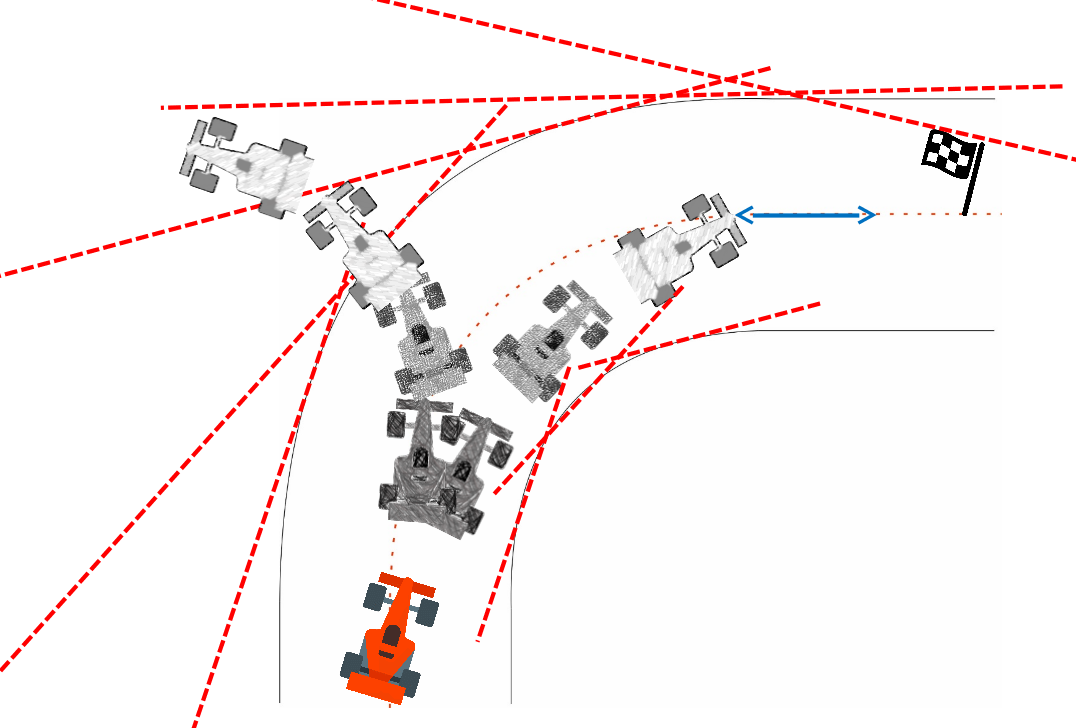
\includegraphics[width=250pt]{Abbildungen/curveAnomaly.png}
	\caption{Fehlerhaftes Verhalten in Spitzkurven}
	\label{fig:curveAnomaly}
\end{figure}
Diese ermöglicht eine höhere Geschwindigkeit. Bei der Berechnung der tangentialen Beschränkung für den nächsten \ac{MPC}-Durchlauf liegen jetzt jedoch alle Tangenten nahezu auf einem Punkt und verhindern daher das Ausscheren des Rennautos. Die daher entstehende neue optimale Trajektorie entspricht wieder nahezu der ursprünglichen. Der resultierende Dreierzyklus wird im schlechtesten Fall solange durchlaufen, bis das Fahrzeug eine der Tangenten trifft und die Optimierung abgebrochen wird.\\
Um dieses Verhalten zu verhindern, wird für diese Kostenfunktion eine zusätzliche Suchbereichsbeschränkung eingeführt. Diese legt um die Prädiktionsschritte der letzten Optimierung einen Kreis zur Einschränkung des Suchbereiches. Ziel ist es, keine so stark abweichende Trajektorie mehr entstehen zu lassen. Es ist darauf zu achten, dass das Fahrzeug trotzdem in den Grenzen seines Fahrzeugmodells keine Beschränkung erfährt. 

Die Suchbereichseinschränkung ist nur für die Kostenfunktion zum Maximieren der Geschwindigkeit benötigt worden.

\subsubsection*{Elastische Distanzminimierung}
Der Nachteil der oben aufgeführten Kostenfunktionen ist, dass sie keinen Spielraum beim Erfüllen der Streckenbeschränkung haben. 
Wenn sowohl das im Simulator wie auch im  \ac{MPC} hinterlegte Fahrzeugmodell exakt gleich sind, kann das virtuelle Rennauto in der Simulationsumgebung bis an die Streckenbegrenzung heranfahren. In der Realität würde eine solche Kostenfunktion das Fahrzeug jedoch zu nah an die Pylonen heranführen. Bei den kleinsten Regelfehlern, Kontaktverlust mit der Fahrbahn (Rutschen), Abweichungen vom Fahrzeugmodell etc. würde das Rennauto vom Kurs abkommen und damit der initiale Fahrzeugzustand ungültig für den Optimierer werden. Um dieses Problem zu umgehen, wird eine neue Art der Kostenfunktion eingeführt, die die Ungleichheitsbedingung der Streckenbegrenzung ersetzt. Dafür wird eine der oberen Funktionen durch einen Kostenanteil erweitert, der wächst, sobald sich das Fahrzeug vom Mittelpunkt der Fahrbahn nach außen hin bewegt. Das Verhältnis der einzelnen Kostenanteile wird der kombinierten Kostenfunktion  
\begin{equation}
	f(\vec{x}) = a \left(\sum_{1}^{N} v_i \right) + \left(\sum_{1}^{N} g \left(h \left(\vec{x}_i \right) \right) \right)
\end{equation}
durch den Parameter a beeinflusst. 
Die Funktion $g(d)$ dient als Platzhalter für verschiedene Gewichtungsfunktionen. Die Funktion $h(\vec{x}_i)$ berechnet die Distanz \(d\) vom Mittelpunkt der Strecke genauso wie bei den tangentialen Beschränkungen in Abschnitt \ref{trackAndPosConstraint}. Mögliche Funktionen sind:

\begin{eqnarray}
	g_1(d) = &\alpha d^2 \\
	g_2(d) = &e^{\alpha (k_1 + d)} + e^{-\alpha(k_2 + d)} \label{eq:distMeasure1}\\
	g_3(d) = &|\frac{\alpha}{k_1-d} + \frac{\alpha}{k_2 - d}| \label{eq:distMeasure2}
\end{eqnarray}
Die Parameter $\alpha$, $k_1$ und $k_2$ dienen zum Variieren der Scheitelpunkte und Steigung.
Mögliche Graphen der Gleichungen sind zur Veranschaulichung in Abbildung \ref{fig:elasticCost} dargestellt.

\begin{figure}[ht!]
	\centering
	
\begin{tikzpicture}
\begin{axis}[
width = 0.8\textwidth,
xmin= -3,
xmax= 3,
ymax = 50,
ylabel=Kosten,
xlabel=Distanz von der Mitte in m]

\addplot [color=blue, mark=none, line width=0.5mm] table [x index=0, y index=2]{Data/costFunct.dat};
\addplot [color=green, mark=none, line width=0.5mm] table [x index=0, y index=3]{Data/costFunct.dat};
\addplot [color=orange, mark=none, line width=0.5mm] table [x index=0, y index=4]{Data/costFunct.dat};

\addlegendentry{Quadratische-Funktion};
\addlegendentry{Alpha-Funktion};

\addlegendentry{E-Funktion};

\end{axis}
\end{tikzpicture} 
	\\
	\ref{named}
	\caption{Verschiedene Distanzmaße um das Verhalten der Trajektorienplanung zu beeinflussen}
	\label{fig:elasticCost}
\end{figure}

Die Idee der Funktionen (\ref{eq:distMeasure1}) und (\ref{eq:distMeasure2}) ist die uneingeschränkte Bewegung des Rennautos auf der ganzen Breite der Strecke. Der Kostenanteil der Distanz von der Mitte wird also bis zum Erreichen der Streckenbegrenzung nahezu vernachlässigt. Erst beim Erreichen des Fahrbahnrandes werden die Kosten sehr schnell extrem groß. Bestenfalls stellen also diese Kostenfunktionen die tangentialen Begrenzungen ideal nach. Die quadratisch wachsende Funktion soll ebenfalls betrachtet werden. Es gilt zu untersuchen, ob bei gesenktem Rechenaufwand eine erfolgreiche Regelung möglich wäre.

\chapter{Simulationsumgebung}
Um die Funktion des \ac{MPC}-Algorithmus verifizieren zu können, wurde eine Simulationsumgebung entwickelt. Der Aufbau ist dreigeteilt: Eine Fahrzeugsimulation berechnet mit austauschbaren Fahrzeugmodellen die Bewegung des Rennautos abhängig von Steuereingaben und einem $\Delta t$. Der Regelanteil in Form des \ac{MPC}-Algorithmus und eine Visualisierung auf Basis einer Spiele-Engine welche auch die zeitlichen Abläufe kontrolliert. 

\section{Python}

Zu Beginn der Arbeit wurde die Programmiersprache Python verwendet, um den \ac{MPC}-Ansatz zu programmieren. Der Vorteil dieser Sprache ist das schnelle Prototyping. Als Optimierer wurde ein \ac{SLSQP}-Algorithmus verwendet. Dieser ist direkt in die SciPy-Bibliothek \cite{Scipy} integriert und unterstützt nichtlineare Nebenbedingungen mit denen sich das \ac{MPC}-Problem zur Fahrzeugregelung abbilden lässt. Solange die Anzahl der Prädiktionsschritte zehn nicht überschreitet, ist die Ausführungszeit gering genug, um eine Aktualisierungsrate von 20 Hz zu erreichen. Bei größeren Prädiktionsvektoren steigt die Berechnungszeit sehr schnell an. Der Benchmark in Abbildung \ref{fig:pythonBench} ist für das fertige Optimierungsproblem gemessen worden.
\begin{figure}[ht!]
	\centering
	
\begin{tikzpicture}
\begin{axis}[
width = 0.8\textwidth,
ylabel=Ausführungszeit in s,
xlabel=Prädiktionsschritte (N)]

\addplot [color=red, mark=x, line width=0.5mm] table [x index=0, y index=1]{Data/pythonBench.dat};
\end{axis}
\end{tikzpicture} 
	\caption{Ausführungszeiten für verschieden  große Horizontlängen}
	\label{fig:pythonBench}
\end{figure}
Dies liegt daran, dass der \ac{SLSQP}-Algorithmus nicht für nichtlineare Probleme ausgelegt ist. Eine bessere Skalierung wird durch einen Lösungsalgorithmus erreicht, der das Innere-Punkte-Verfahren nutzt. Dieser Algorithmus setzt jedoch für eine gute Performance die Kenntnis über die Ableitung der Systemfunktion voraus. Auf diesen Sachverhalt wurde bereits im Abschnitt \ref{ipm} eingegangen. Die automatische Ableitung kann mit Frameworks wie CasADi \cite{CasADi}, PyADOL-C \cite{PYADOLC}, PyCppAD \cite{CppAD} berechnet werden \cite{DBLP:journals/corr/TurkinT16}. 
Eine Implementierung des \ac{MPC}-Ansatzes in CasADi wurde  aufgrund der schlechten Dokumentation abgebrochen und es wurde nach einer Alternativlösung gesucht. Das Ergebnis dieser Suche führte zur Verwendung einer neuen Programmiersprache. 


\section{Julia}
\label{julia}
Julia ist die Programmiersprache, die eine Umsetzung des \ac{MPC}-Algorithmus effizient und performant ermöglicht. Sie wurde im Jahr 2009 von Jeff Bezanson, Stefan Karpinski, Viral B. Shah, und Alan Edelman ersonnen und ist damit noch eine sehr junge Sprache. Sie ist vor allem für numerische Analysen und wissenschaftliche Berechnungen entworfen worden und bietet in diesen Bereichen viele Funktionalitäten. Ebenfalls ein wichtiges Ziel bei der Entwicklung war es, ohne vorheriges Kompilieren sehr schnell zu sein und trotzdem weiterhin das general-purpose Paradigma zu erfüllen. Ein Vergleich der Berechnungsgeschwindigkeit verschiedener Sprachen bezüglich viel genutzter Funktionen im wissenschaftlichen Umfeld ist in der Abbildung \ref{fig:juliaBench} zu sehen.

\begin{figure}[ht!]
	\centering
	
\begin{tikzpicture}
\begin{axis}[
width = 1.0\textwidth,
height = 0.6\textwidth,
ymin=-1e0, ymax=1e1,
ylabel=Ausführungszeiten relativ zu C,
x tick label style={font=\small,text width=1.2cm,align=center},
xticklabels={Benchmark,C,Julia,LuaJIT,Go,Fortran,Java,Java-script,Matlab,Mathe-matica, Python},
legend pos=north west]

\addplot [color=red, only marks] table [x index=0, y index=1]{Data/juliaBench.dat};
\addplot [color=blue, only marks] table [x index=0, y index=2]{Data/juliaBench.dat};
\addplot [color=green, only marks] table [x index=0, y index=3]{Data/juliaBench.dat};
\addplot [color=black, only marks] table [x index=0, y index=4]{Data/juliaBench.dat};
\addplot [color=orange, only marks] table [x index=0, y index=5]{Data/juliaBench.dat};
\addplot [color=yellow, only marks] table [x index=0, y index=6]{Data/juliaBench.dat};
\addplot [color=purple, only marks] table [x index=0, y index=7]{Data/juliaBench.dat};
\addplot [color=brown, only marks] table [x index=0, y index=8]{Data/juliaBench.dat};
\addlegendentry{iteration pi sum}
\addlegendentry{recursion fibonacci}
\addlegendentry{recursion quicksort}
\addlegendentry{parse integers}
\addlegendentry{print to file}
\addlegendentry{matrix statistics}
\addlegendentry{matrix multiply}
\addlegendentry{mandelbrot}
\end{axis}
\end{tikzpicture} 
	\caption{Ausführungszeiten für verschiedene Sprachen}
	\label{fig:juliaBench}
\end{figure}

Die wichtigsten Feautres von Julia sind:

\begin{itemize}
	
	\item Funktionsüberladung (eng.: multiple dispatch)\\Wird genutzt um die gleiche Methode für verschiedene Kombinationen an Eingabeparametern oder Variablentypen zu überladen. Bei dem Funktionsaufruf wird die passende Methodendefinition aufgerufen. \\
	\item Datentyp detektion (eng.:type inference) \\Das automatische Detektieren des Datentyps. Dies befreit den Programmierer vom Festlegen des Typs und ermöglicht trotzdem Typprüfung. \\
	\item \ac{JIT} Kompilierer\\ Ein System, in dem ein \ac{JIT} Kompilierer implementiert ist, wandelt den Computer Code erst zur Laufzeit in Bytecode um. 
	Der große Vorteil liegt in der kontinuierlichen Analyse während der Ausführung. Dadurch können Bereiche ausfindig gemacht werden, die durch ein Neukompilieren eine signifikante Verbesserung bei der Ausführungszeit erfahren würden. \\
\end{itemize}
Es wäre möglich die einzelnen benötigten Bestandteile für einen \ac{MPC}-Algorithmus in Julia zu implementieren. Jedoch gibt es eine umfangreiche Erweiterung, welche eine passende Schnittstelle für solche Probleme zur Verfügung stellt.

\subsubsection*{Jump}
\ac{Jump} ist eine Bibliothek für Julia mit der sich mathematische Probleme modellieren und lösen lassen. Es besitzt Schnittstellen für mehrere sowohl frei verfügbare, wie auch kommerzielle Optimierer, mit denen lineare oder nichtlineare Probleme modelliert und gelöst werden können. Der große Vorteil von \ac{Jump} ist, dass die Definition des mathematischen Problems unabhängig von dem verwendeten Optimierer ist und dieser damit leicht ausgetauscht werden kann (siehe Schaubild \ref{fig:jumpDiagram}). Ebenfalls ein großer Vorteil ist die direkt berechnete automatische Ableitung in \ac{Jump}. Der Programmierer spart sich dadurch sehr viel Arbeit.

\begin{figure}[ht!]
	\centering
	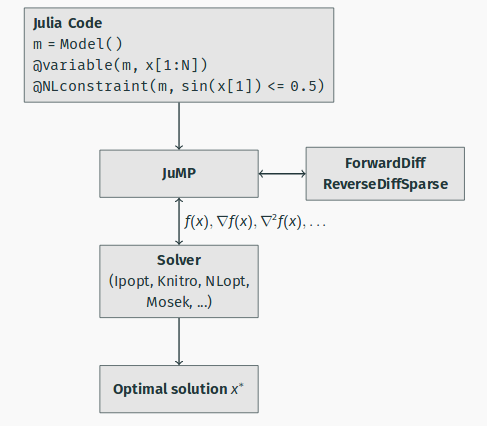
\includegraphics[width=150pt]{Abbildungen/jumpDiagram.png}
	\caption{Blockdiagramm von \ac{Jump}. Wichtige Vorteile sind die automatische Ableitung und das einfache Tauschen von Optimierern}
	\label{fig:jumpDiagram}
\end{figure}

Die Definition der Optimierungsprobleme wird in Jump mit einer Syntax vorgesehen, die der standardmäßigen mathematischen Definition ähnelt. Die Integration gestaltet sich daher sehr intuitiv.  Zudem existiert eine ausführliche Dokumentation.
Obwohl \ac{Jump} Schnittstellen zu vielen verschiedenen Optimierern besitzt, ist nur der \ac{Ipopt} frei nutzbar und dafür ausgelegt nichtlineare Nebenbedingungen zu berücksichtigen. Die Verwendung von \ac{Jump} und \ac{Ipopt} führen zu einer deutlich besseren Skalierung und Laufzeit (siehe \ref{runtime}) als der \ac{SLSQP}-Ansatz in Python. Die Abbruchbedingung in \ac{Ipopt} wurde auf $1e-1$ festgelegt.


\section{\acl{SFML}}
Die Basis für die Simulation bildet die \ac{SFML}, die für die grafischen Darstellungen des Kurses, Rennauto, Prädiktionsschritte und Fahrzeuginformationen genutzt wird. Ein Bildschirmfoto der Simulation ist in Abbildung \ref{fig:simVisual} dargestellt.
\begin{figure}[ht!]
	\centering
	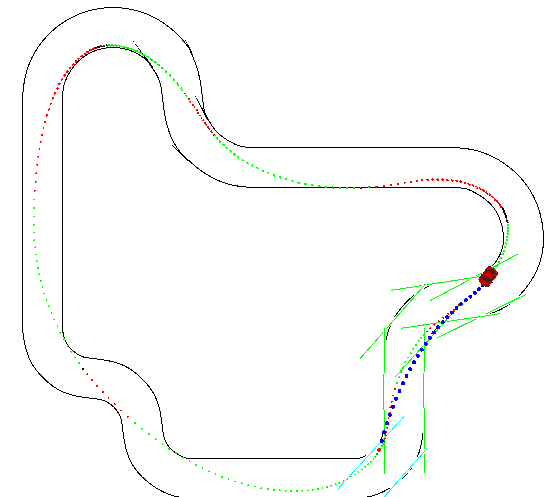
\includegraphics[width=350pt]{Abbildungen/sim_visual.png}
	\caption{Grafische Darstellung des MPC - Algorithmus in der Simulationsumgebung}
	\label{fig:simVisual}
\end{figure} 
Zusätzlich zur Visualisierung, stellt die Spiele-Engine auch sicher, dass die zeitlichen Abläufe eingehalten werden. Das Grundprinzip ist eine einzige unendlich laufende Schleife, die mit einer vorher festgelegten Wiederholungsrate ausgeführt wird. Benötigen die Berechnungen innerhalb dieser Schleife länger als das angegebene
$\Delta t =  \frac{1}{20}$ s, sinkt die Ausführungsrate, überschritten wird sie jedoch nie. Die Schritte, die innerhalb dieser Schleife abgearbeitet werden, sind das Abfragen möglicher Eingaben des Nutzers oder Ereignisse der einzelnen Objekte. Im zweiten Schritt werden alle Berechnungen der eigentlichen Fahrzeugsimulation und \ac{MPC}-Algorithmus ausgeführt und im letzten Schritt werden die grafischen Elemente erstellt und angezeigt. Wie für eine Spiele-Engine üblich, befindet sich der Ursprung des Koordinatensystems in der linken oberen Ecke. Die y-Achse ist daher entgegengesetzt zu dem in der Fahrzeugsimulation verwendeten Standardachsenaufbau orientiert. Zudem werden Distanzen in der Engine nur in Pixeln gemessen. Es wurden daher zwei Parameter eingeführt, welche die Fenstergröße in Pixeln festlegen (in \(x\)- und  \(y\)-Richtung) und zusätzlich eine Angabe wie vielen Metern dieser jeweils in Pixeln entspricht. Die daraus resultierenden Verhältnisse 
\begin{eqnarray}
	scaleX = \frac{windowSizeXinPixel}{windowSizeXinM} \\
	scaleY = - \frac{windowSizeYinPixel}{windowSizeYinM} 
\end{eqnarray}

werden verwendet, um alle Größenverhältnisse einheitlich in der Simulation zu halten und eine realistische Visualisierung zu gewährleisten. 
Die Größe des Bereichs in dem der Rennkurs abgesteckt wird und die Fenstergröße zur Darstellung der Simulation können durch Parameter angepasst werden. Zusätzlich wurde ein Offset eingeführt, welcher die Nullpunkte der \(x\)- und \(y\)-Position im Koordinatensystem verschiebt. Damit kann der Ursprung des Koordinatensystems der Fahrzeugsimulation beliebig im Anzeigebereich verschoben werden. 
Der Aufbau ist in dem Blockdiagramm \ref{fig:block_diagram_sim} nochmals zusammengefasst. 
\begin{figure}[ht!]
	\centering
	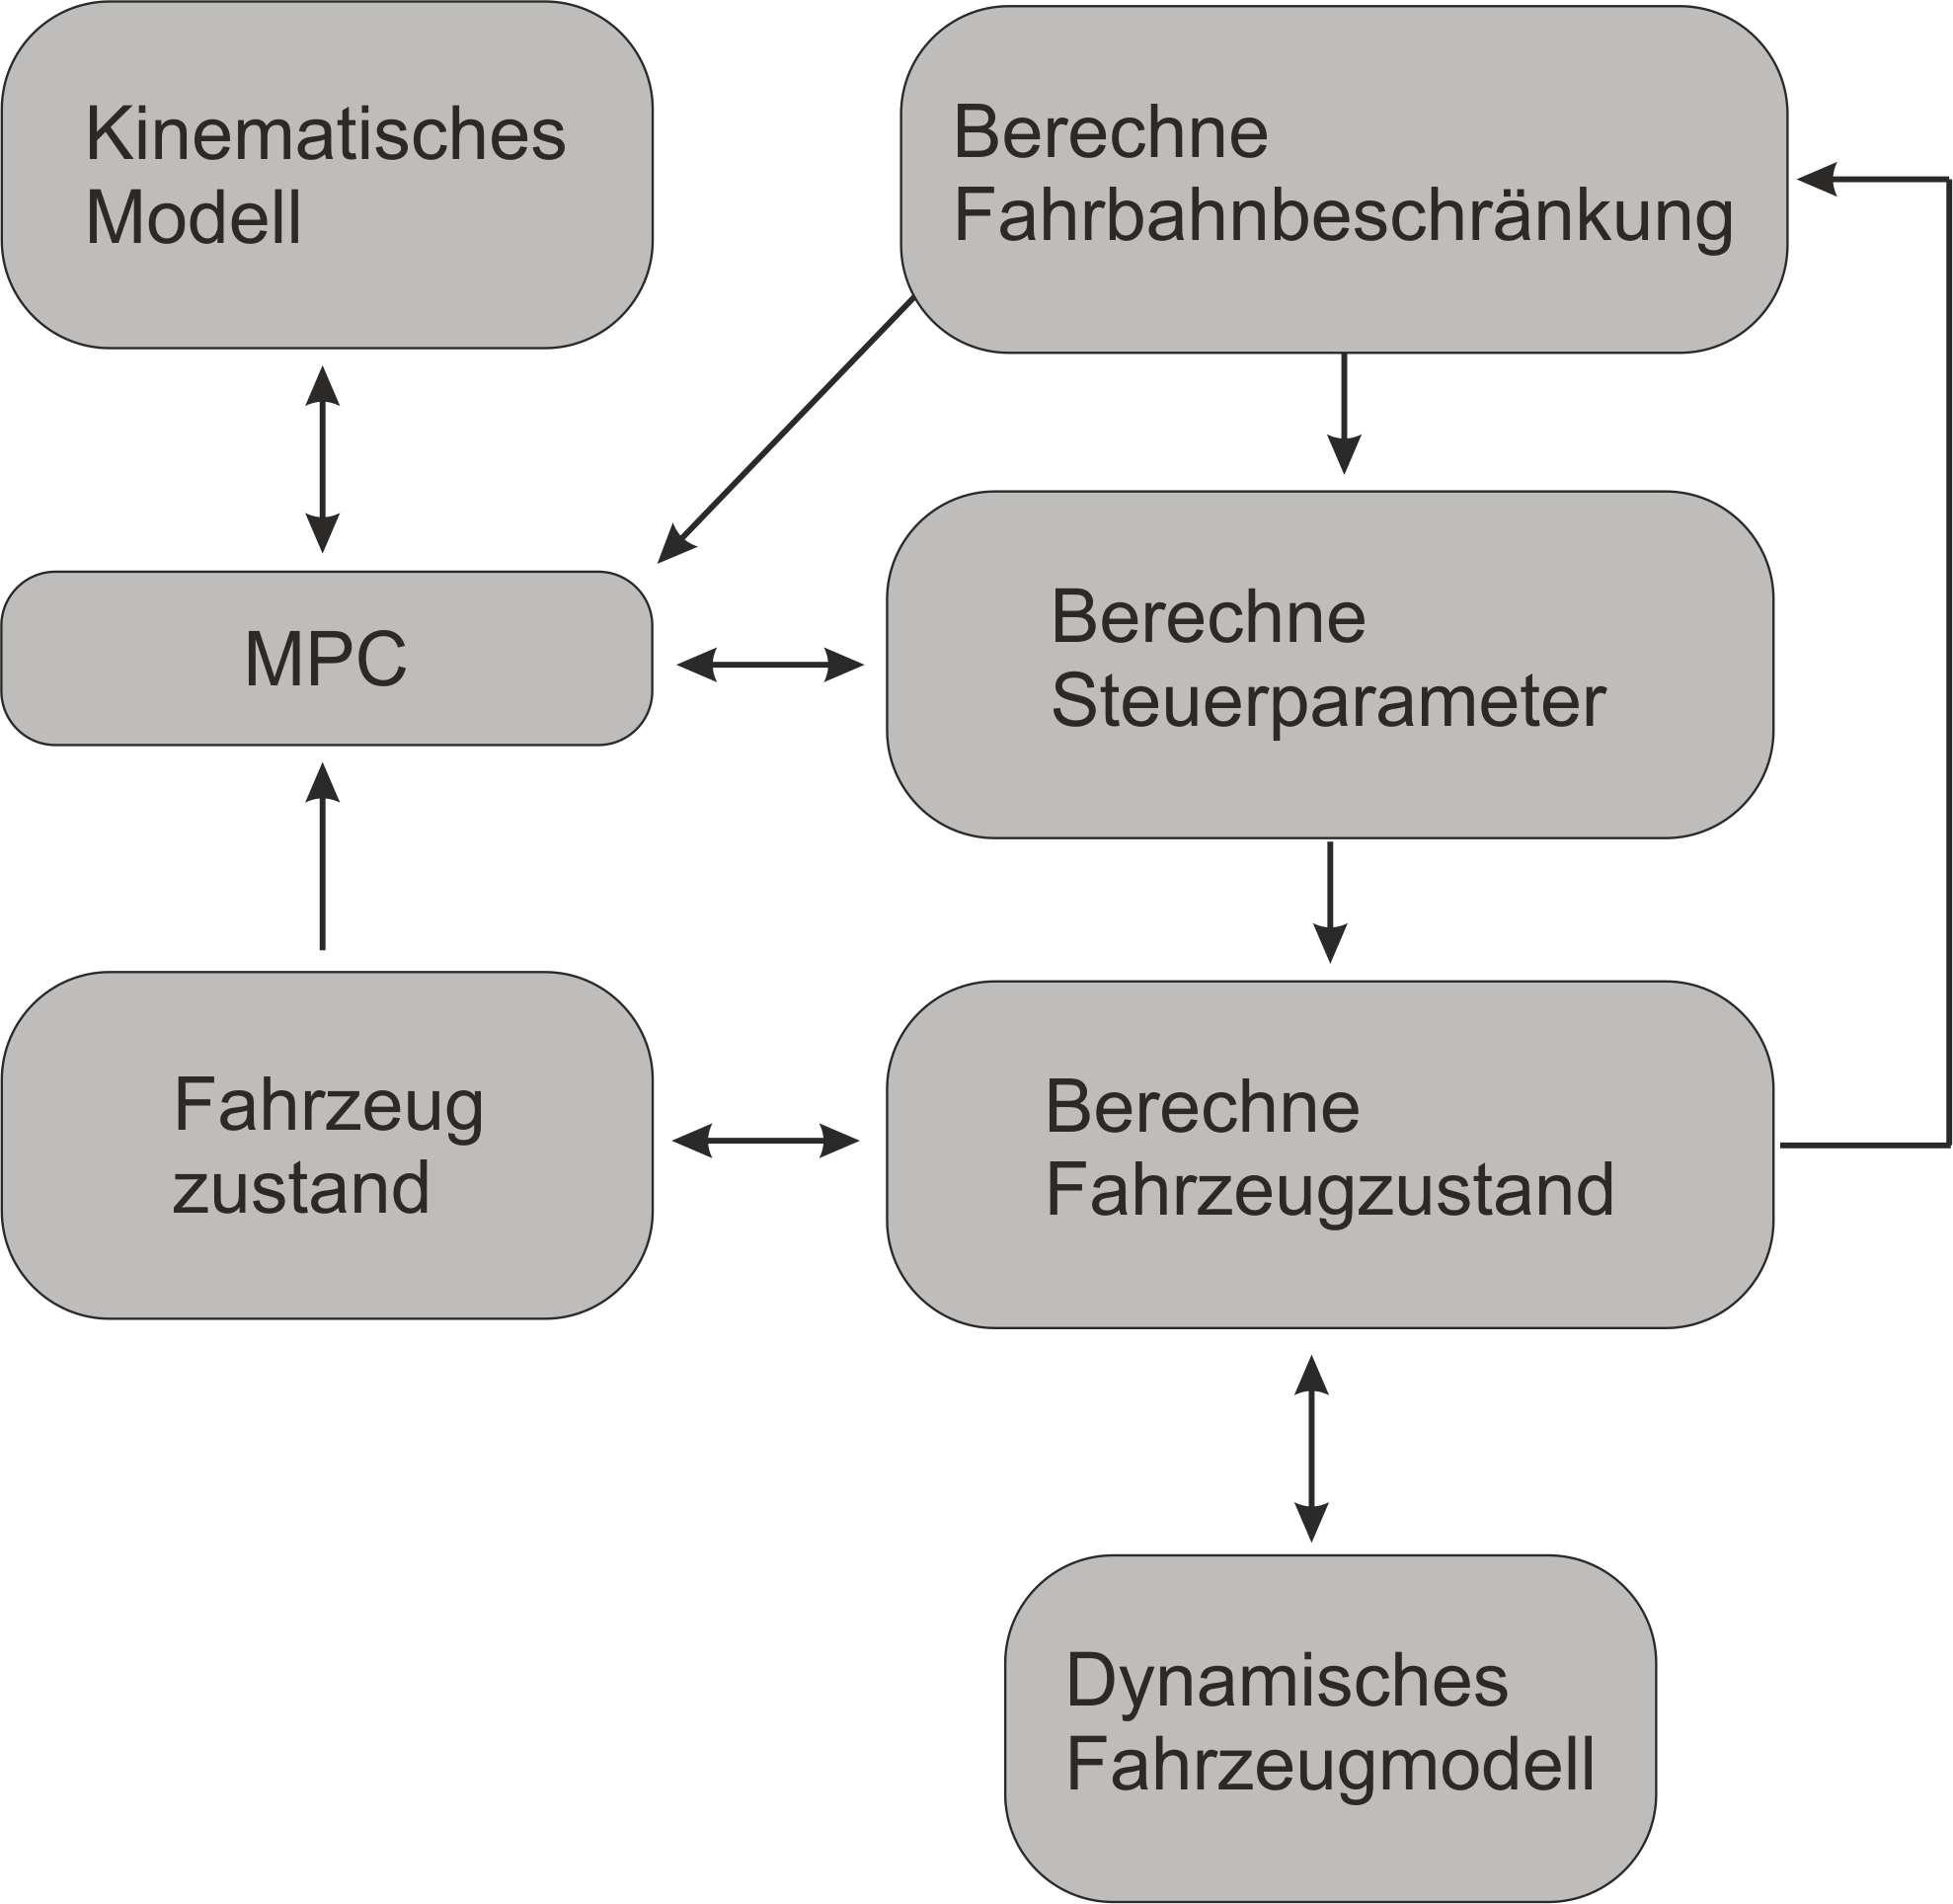
\includegraphics[width=250pt]{Abbildungen/MPCSimulation.png}
	\caption{Blockdiagramm der Simulation mit dem \ac{MPC}-Algorithmus}
	\label{fig:block_diagram_sim}
\end{figure}
Der Simulator berechnet abhängig vom aktuellen Fahrzeugzustand die Streckenbegrenzungen und hinterlegt diese zusammen mit dem Fahrzeugzustand im \ac{MPC}-Algorithmus. Im nächsten Schritt errechnet der Optimierer die Steuerparameter für den Prädiktionshorizont. Zusammen mit dem dynamischen Fahrzeugmodell und den Steuerparametern, wird der neue Fahrzeugzustand berechnet und der nächste Durchlauf der Simulationsschleife gestartet.

\section{Virtueller Rennkurs}
Wie in der Einführung bereits erwähnt, ist das Ziel der Arbeit ein \ac{MPC}-Algorithmus zu entwickeln mit dem die Trackdrive-Disziplin möglichst schnell abgefahren werden kann. Die Grundvoraussetzung für diese Arbeit ist die bereits vollständig erstellte Karte des Rennkurses und eine Lokalisierung innerhalb dieser Karte. Die Updaterate für diese Positionsschätzung wird mit 20 Hz angenommen. Das Ziel ist es also, die Regelparameter mit einem $\Delta t$ von $\frac{1}{20}$ s für das Rennauto berechnen zu können.  Zum Testen der Algorithmen wurde ein beliebiger Kurs definiert, welcher sich an die Vorgaben des Regelwerkes hält und damit einen minimalen Kurvenradius von 9 m, Maximallänge einer Geraden von 80 m und maximal 180° Spitzkurven besitzt. Die Strecke wird als kubischer Spline hinterlegt. Bei einem Spline (auch Polynomzug), handelt es sich um eine Funktion, die stückweise aus Polynomen zusammengesetzt ist. Kubische Splines werden unter anderem zur Berechnung des Bahnverlaufes bei Achterbahnen verwendet, um ruckartige Beschleunigungswechsel für die Fahrgäste zu vermeiden. Auch beim Entwurf von Kurven und Oberflächen sind Splines von Bedeutung. Die Stützpunkte werden durch das Zusammensetzen von verschiedenen Streckenelementen erzeugt. Der Vorteil ist das schnelle und einfache erstellen beliebiger Strecken. 

\chapter{Evaluierung}
\section{Modellfehler}
\label{modelError}
Ohne eine Verifizierung der Plausibilität der implementierten Modelle, ist keine systematische Untersuchung möglich. Hierfür wurden die zwei Disziplinen \text{acceleration} und \text{skidpad} gewählt und die besten gefahrenen Ergebnisse des Rennautos des High-Octane Motorspors als Vergleichsbasis genutzt.


\subsection{Disziplin Acceleration}
In dieser Disziplin ist es das Ziel der Teams eine $75$ m lange, gerade Strecke in möglichst kurzer Zeit zurückzulegen.
Es werden drei verschiedene longitudinale Konfigurationen des Fahrzeugmodells evaluiert. Zuerst das kinematische Modell in dem die maximale mittlere Beschleunigung (\ref{long_acc_kin}) aus den Fahrzeugdaten errechnet wird. Das zweite untersuchte Modell, basiert auf der Leistung des Motors und der maximal übertragbaren Kraft der Reifen (\ref{long_dyn_engine}).
Das dritte Modell betrachtet zusätzlich zur Motorleistung, Rollreibung und Luftwiderstand. 

\begin{figure}
	\centering
	\pgfplotstabletypeset{Grafiken/accdec.dat}



\begin{tikzpicture}
\begin{axis}[
xlabel=Q Series,
ylabel=P Values]
\addplot table [y=P, x=$Q1$]{data.dat};

\end{axis}
\end{tikzpicture} 
	\ref{accdeccLegend}
	\caption{Geschwindigkeitsverlauf bei maximaler Beschleunigung für verschiedene longitudinale Modelle}
	\label{fig:accdec}
\end{figure}
Zuerst werden die Beschleunigungskurven betrachtet. Hierfür wird mit allen hinterlegten Modellen fünf Sekunden lang maximal beschleunigt und direkt danach $2,5$ s mit maximaler Kraft gebremst.
In der Grafik \ref{fig:accdec} wird deutlich, wie stark sich die einzelnen Modelle, obwohl sie sich auf das gleiche Fahrzeug beziehen, voneinander unterscheiden. Das Fahrzeug besitzt eine Maximalgeschwindigkeit von $121$  $\frac{\text{km}}{\text{h}}$, welche durch die Übersetzung im Getriebe limitiert wird. Das kinematische Modell trifft mit seiner durchschnittlichen Beschleunigung exakt die gefahrenen Testwerte. Da aber die dynamischen Modelle eine größere Anfangsbeschleunigung haben und vom kinematischen Modell, hinterlegt im \ac{MPC}, geregelt werden, wird die Beschleunigung im kinematischen Modell so angepasst, dass es die gleiche Anfangssteigung besitzt. Die Steigung beträgt $24$ $ \frac{\text{m}}{\text{s\textsuperscript{2}}}$. 
Als nächstes wird die Zeit über eine Strecke von $75$ m gemessen. Das Ergebnis für das kinematische Modell, mit angepasster Beschleunigungskurve, ist $3,0$ Sekunden. Dieser Wert ist, wie bereits zu erwarten war, deutlich zu schnell. Realistische Werte liegen zwischen $3,8$ und $4,5$ Sekunden, je nach Fähigkeiten des Fahrers, Wetterbedingungen und Reifentemperatur. Das dynamische Modell, das keinerlei Reibung berücksichtigt, ist ebenfalls mit $3,45$ Sekunden zu schnell. Mit Reibung entsteht ein realistischer Wert von $4,3$ Sekunden, was typischen Messzeiten für das Fahrzeug des High-Octane Motorspors e.V. entspricht. Für ein gutes longitudinales Modell des Fahrzeugs, muss also der Luftwiderstand, der einen deutlich größeren Anteil auf die Gesamtreibung hat als der Rollwiderstand, berücksichtigt werden. Die Rollreibung ist bei maximaler Geschwindigkeit um den Faktor 100 kleiner als die aerodynamischen Kräfte und entspricht etwa 6 und 592 N respektive. Im Folgenden, wird immer das um Reibung erweiterte longitudinalen Modell verwendet.


\subsection{Disziplin Skidpad}
In dieser Disziplin fährt das Fahrzeug eine liegende 8. Der limitierende Faktor ist also die maximale Querbeschleunigung, welche das Rennauto noch auf dem Kurs hält. In der Simulation wird vereinfacht von einem Rundkurs, welcher in Abbildung \ref{fig:roundCourse} dargestellt wird, mit dem Außendurchmesser von $21,25$ m ausgegangen. 
\begin{figure}
	\centering
	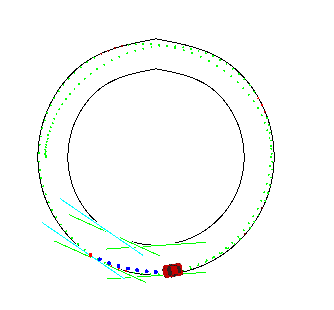
\includegraphics[width=200pt]{Abbildungen/roundCourse.png}
	\caption{Rundkurs zum Messen der maximalen Querbeschleunigung}
	\label{fig:roundCourse}
\end{figure}
Ob die Begrenzung der Querbeschleunigung (\ref{limitLatAcc}) mit der Simulation übereinstimmt, kann durch die wirkende Querbeschleunigung überprüft werden.
Diese berechnet sich aus Bahngeschwindigkeit $v$ und dem Radius der Kreisbahn $r$. 
\begin{equation}
	a = \frac{v^2}{r}
\end{equation}

Die Bahngeschwindigkeit wird durch die Kreisfrequenz $\omega$ berechnet.
\begin{eqnarray}
	 \omega = 2 \pi f \\
	 v = r \cdot \omega
\end{eqnarray}


Für das in der Simulationsumgebung hinterlegte kinematische Modell ist die gemessene Rundenzeit $4,65$ s. Daraus lässt sich eine Durchschnittsgeschwindigkeit $ v= 13.9$ $ \frac{\text{m}}{\text{s}}$ berechnen, was einer Querbeschleunigung von $a = 19.37$ $ \frac{\text{m}}{\text{s\textsuperscript{2}}}$ entspricht. Das im Fahrzeugmodell hinterlegte $a_{max}$ ist mit $19,62$ $ \frac{\text{m}}{\text{s\textsuperscript{2}}}$ also sehr nah an dem in der Simulation erfahrenen werten. Die Differenz zu der schnellsten gemessenen Runde mit dem echten Fahrzeug ($4,77$ s) lässt sich dadurch erklären, dass der MPC-Algorithmus die ideale Stellgrößen berechnet und damit auch einen idealen Rundkurs abfährt. Zudem wurde die maximal gemessene Querbeschleunigung des Fahrzeugs als $a_{max}$ gewählt, diese kann in der Realität nicht durchgängig gehalten werden. Der Wert wurde beim Einlenken mit hoher Geschwindigkeit ermittelt, in diesem Fall besitzt das Rennauto, aufgrund seiner Aerodynamik, einen hohen Abtrieb. Durch die höhere Normalkraft welche die Reifen auf die Straße presst, können größere laterale Kräfte gewirkt werden.
Für das dynamische Fahrzeugmodell wurde eine minimale Rundenzeit 3,35 s gemessen.  Die damit erhaltene maximale Querbeschleunigung ist deutlich größer als die des kinematischen Modells. Die Differenz ist auf eine zu stark vereinfachte Annahme der Reifenkräfte zurückzuführen. Die lateralen Kräfte, welche durch die \ac{M.F.} errechnet wurden, werden verdoppelt, da das Fahrzeug in der Realität jeweils zwei Räder pro Achse besitzt. In schnell gefahrenen Kurven verlagert sich jedoch die Gewichtskraft des Rennautos, welche den Reifen auf die Straße presst, stark auf das kurvenäußere Rad. Die vom kurveninneren Rad maximal übertragbare Kraft bricht daher deutlich ein. Die Kraft, welche der Reifen maximal übertragen kann, steigt zwar mit höherer Normalkraft an, jedoch ist der Zusammenhang nichtlinear und nähert sich immer mehr einem maximalen Wert an. Das kurvenäußere Rad kann daher den Verlust des inneren Reifen nicht kompensieren. Dieser Zusammenhang ist die Grundlage für das Verwenden eines Stabilisators im Fahrzeug. Er verringert den Effekt und führt zu einem besseren Fahrverhalten.



Da im Skidpad die Querbeschleunigung konstant ist, spielt das Trägheitsmoment in dieser Disziplin eine untergeordnete Rolle.
Ein deutlich dynamischeres Szenario soll die Unterschiede zwischen kinematischem und dynamischen Szenario besser veranschaulichen.

\subsection{Modellabhängige Veränderung der Orientierung}
In der Darstellung \ref{fig:modelDiffOrient} ist die Änderung der Orientierung für einen oszillierenden Lenkwinkel veranschaulicht. Es werden die vier verschiedenen Geschwindigkeiten $7$, $14$, $21$ und $28$ $\frac{\text{m}}{\text{s}}$ ohne jegliche longitudinale Beschleunigung getestet. Dies soll einen guten Überblick über den gesamten Geschwindigkeitsbereich ermöglichen.

\begin{figure}
	\centering
	\subfigure{
		\begin{tikzpicture}
\begin{axis}[
height = 0.250\textwidth,
width = 0.465\textwidth,
xmin= 0,
xmax = 2.0,
ymin = -0.6,
ymax = 0.6,
ylabel=Lenkwinkel in rad]
\addplot [color=black, mark=none, line width=0.5mm] table [x index=0, y index=1]{Data/modelDiffOrient/modelDiffOrientNoAcc7.dat};

\end{axis}
\end{tikzpicture} 
	}%NOLINE
	\subfigure{
		\begin{tikzpicture}
\begin{axis}[
height = 0.250\textwidth,
width = 0.465\textwidth,
xmin= 0,
xmax = 2.0,
ymin = -0.6,
ymax = 0.6]
\addplot [color=black, mark=none, line width=0.5mm] table [x index=0, y index=1]{Data/modelDiffOrient/modelDiffOrientNoAcc7.dat};
\end{axis}
\end{tikzpicture} 
	}	
	
	\subfigure[7 $\frac{\text{m}}{\text{s}}$]{
		\begin{tikzpicture}
\begin{axis}[
width = 0.47\textwidth,
xmin= 0,
xmax = 2.0,
ymin = 0.0,
ymax= 0.8,
ylabel= Orientierung in rad,
legend columns = 3,
legend entries = {kin. Modell;,dyn. Modell;, dyn. mit K.K.},
legend to name =modelDiffOrientLegend
]
\addplot [color=red, mark=none, line width=0.5mm] table [x index=0, y index=2]{Data/modelDiffOrient/modelDiffOrientNoAcc7.dat};
\addplot [color=blue, mark=none, line width=0.5mm] table [x index=0, y index=3]{Data/modelDiffOrient/modelDiffOrientNoAcc7.dat};
\addplot [color=green, dashed, mark=none, line width=0.5mm] table [x index=0, y index=4]{Data/modelDiffOrient/modelDiffOrientNoAcc7.dat};

\end{axis}
\end{tikzpicture} 
		\label{fig:modelDiffOrient7}
	}%NOLINE
	\subfigure[14 $\frac{\text{m}}{\text{s}}$]{
		\begin{tikzpicture}
\begin{axis}[
width = 0.47\textwidth,
xmin= 0,
xmax = 2.0,
ymin = 0.0,
ymax= 0.9]
\addplot [color=red, mark=none, line width=0.5mm] table [x index=0, y index=2]{Data/modelDiffOrient/modelDiffOrientNoAcc14.dat};
\addplot [color=blue, mark=none, line width=0.5mm] table [x index=0, y index=3]{Data/modelDiffOrient/modelDiffOrientNoAcc14.dat};
\addplot [color=green, dashed, mark=none, line width=0.5mm] table [x index=0, y index=4]{Data/modelDiffOrient/modelDiffOrientNoAcc14.dat};

\end{axis}
\end{tikzpicture} 
		\label{fig:modelDiffOrient14}
	}
	\subfigure[21 $\frac{\text{m}}{\text{s}}$]{
		\begin{tikzpicture}
\begin{axis}[
width = 0.47\textwidth,
xmin= 0,
xmax = 2.0,
ymin = 0.0,
ymax= 0.8,
xlabel= Zeit in s,
ylabel= Orientierung in rad,]
\addplot [color=red, mark=none, line width=0.5mm] table [x index=0, y index=2]{Data/modelDiffOrient/modelDiffOrientNoAcc21.dat};
\addplot [color=blue, mark=none, line width=0.5mm] table [x index=0, y index=3]{Data/modelDiffOrient/modelDiffOrientNoAcc21.dat};
\addplot [color=green,dashed,  mark=none, line width=0.5mm] table [x index=0, y index=4]{Data/modelDiffOrient/modelDiffOrientNoAcc21.dat};
\end{axis}
\end{tikzpicture} 
		\label{fig:modelDiffOrient21}
	}%NOLINE
	\subfigure[28 $\frac{\text{m}}{\text{s}}$]{
		\begin{tikzpicture}
\begin{axis}[
width = 0.47\textwidth,
xmin= 0,
xmax = 2.0,
ymin = 0.0,
ymax= 0.8,
xlabel= Zeit in s]
\addplot [color=red, mark=none, line width=0.5mm] table [x index=0, y index=2]{Data/modelDiffOrient/modelDiffOrientNoAcc28.dat};
\addplot [color=blue, mark=none, line width=0.5mm] table [x index=0, y index=3]{Data/modelDiffOrient/modelDiffOrientNoAcc28.dat};
\addplot [color=green,dashed,  mark=none, line width=0.5mm] table [x index=0, y index=4]{Data/modelDiffOrient/modelDiffOrientNoAcc28.dat};
\end{axis}
\end{tikzpicture} 
		\label{fig:modelDiffOrient28}
	}	
	\ref{modelDiffOrientLegend}
	\caption{Orientierung des Rennautos für eine Sinuskurve als Eingangswert des Lenkwinkels. Es werden verschiedene Geschwindigkeiten ohne longitudinale Beschleunigung betrachtet.}\label{fig:modelDiffOrient}
\end{figure}

Zuerst wird das Verhalten des kinematischen Modells betrachtet. Bei der geringsten Geschwindigkeit von $7$ $\frac{\text{m}}{\text{s}}$ folgt die Orientierung noch genau dem Lenkwinkel nach und erreicht damit den Maximalwert im Nulldurchgang der Sinusfunktion des Lenkwinkels. Mit höheren Geschwindigkeiten begrenzt jedoch immer stärker die Beschränkung der maximalen Querbeschleunigung. Bei $14$ $\frac{\text{m}}{\text{s}}$ ist dies deutlich erkennbar, der Anfangspunkt der Kurve ist noch leicht abgerundet. Dies ist bei $21$ und $28$ $\frac{\text{m}}{\text{s}}$ nicht mehr der Fall. Ab  $14$ $\frac{\text{m}}{\text{s}}$ begrenzt die maximale Querbeschleunigung auch immer stärker die maximal erreichte Orientierung. 

Das Verhalten des dynamischen Modells und das des um den \ac{K.K.} erweiterten sind in diesem Anwendungsfall genau gleich. Dies ist darauf zurückzuführen, dass keinerlei longitudinale Kraft an den Reifen anliegt. Die vom Reifen zu übertragenden Kräfte bewegen sich daher nur auf der x-Achse des \ac{K.K.} und erfahren keine Einschränkung. 
Das Verhalten der dynamischen Modelle bei den unterschiedlichen Geschwindigkeiten ist nicht direkt aus den Gleichungen nachvollziehbar. Aus dem Verlauf der Diagramme wird jedoch deutlich, dass das Trägheitsmoment dazu führt, dass die maximale Orientierung deutlich dem kinematischen Modell und damit dem Lenkwinkel nacheilt. 

\begin{figure}
	\centering
	\subfigure{
		\begin{tikzpicture}
\begin{axis}[
height = 0.250\textwidth,
width = 0.465\textwidth,
xmin= 0,
xmax = 2.0,
ymin = -0.6,
ymax = 0.6,
ylabel=Lenkwinkel in rad]
\addplot [color=black, mark=none, line width=0.5mm] table [x index=0, y index=1]{Data/modelDiffOrient/modelDiffOrientNoAcc7.dat};

\end{axis}
\end{tikzpicture} 
	}%NOLINE
	\subfigure{
		\begin{tikzpicture}
\begin{axis}[
height = 0.250\textwidth,
width = 0.465\textwidth,
xmin= 0,
xmax = 2.0,
ymin = -0.6,
ymax = 0.6]
\addplot [color=black, mark=none, line width=0.5mm] table [x index=0, y index=1]{Data/modelDiffOrient/modelDiffOrientNoAcc7.dat};
\end{axis}
\end{tikzpicture} 
	}	
	\subfigure[7 $\frac{\text{m}}{\text{s}}$]{
		\begin{tikzpicture}
\begin{axis}[
width = 0.47\textwidth,
xmin= 0,
xmax = 2.0,
ymin = 0.0,
ymax= 0.8,
ylabel= Orientierung in rad]
\addplot [color=red, mark=none, line width=0.5mm] table [x index=0, y index=2]{Data/modelDiffOrient/modelDiffOrientMaxAcc7.dat};
\addplot [color=blue, mark=none, line width=0.5mm] table [x index=0, y index=3]{Data/modelDiffOrient/modelDiffOrientMaxAcc7.dat};
\addplot [color=green, mark=none, line width=0.5mm] table [x index=0, y index=4]{Data/modelDiffOrient/modelDiffOrientMaxAcc7.dat};

\end{axis}
\end{tikzpicture} 
		\label{fig:modelDiffOrientMax7}
	}%NOLINE
	\subfigure[14 $\frac{\text{m}}{\text{s}}$]{
		\begin{tikzpicture}
\begin{axis}[
width = 0.47\textwidth,
xmin= 0,
xmax = 2.0,
ymin = 0.0,
ymax= 0.9]
\addplot [color=red, mark=none, line width=0.5mm] table [x index=0, y index=2]{Data/modelDiffOrient/modelDiffOrientMaxAcc14.dat};
\addplot [color=blue, mark=none, line width=0.5mm] table [x index=0, y index=3]{Data/modelDiffOrient/modelDiffOrientMaxAcc14.dat};
\addplot [color=green,dashed , mark=none, line width=0.5mm] table [x index=0, y index=4]{Data/modelDiffOrient/modelDiffOrientMaxAcc14.dat};

\end{axis}
\end{tikzpicture} 
		\label{fig:modelDiffOrientMax14}
	}
	\subfigure[21 $\frac{\text{m}}{\text{s}}$]{
		\begin{tikzpicture}
\begin{axis}[
width = 0.47\textwidth,
xmin= 0,
xmax = 2.0,
ymin = 0.0,
ymax= 0.9,
xlabel= Zeit in s,
ylabel= Orientierung in rad]
\addplot [color=red, mark=none, line width=0.5mm] table [x index=0, y index=2]{Data/modelDiffOrient/modelDiffOrientMaxAcc21.dat};
\addplot [color=blue, mark=none, line width=0.5mm] table [x index=0, y index=3]{Data/modelDiffOrient/modelDiffOrientMaxAcc21.dat};
\addplot [color=green, dashed,  mark=none, line width=0.5mm] table [x index=0, y index=4]{Data/modelDiffOrient/modelDiffOrientMaxAcc21.dat};

\end{axis}
\end{tikzpicture} 
		\label{fig:modelDiffOrientMax21}
	}%NOLINE
	\subfigure[28 $\frac{\text{m}}{\text{s}}$]{
		\begin{tikzpicture}
\begin{axis}[
width = 0.47\textwidth,
xmin= 0,
xmax = 2.0,
ymin = 0.0,
ymax= 0.8,
xlabel= Zeit in s]
\addplot [color=red, mark=none, line width=0.5mm] table [x index=0, y index=2]{Data/modelDiffOrient/modelDiffOrientMaxAcc28.dat};
\addplot [color=blue, mark=none, line width=0.5mm] table [x index=0, y index=3]{Data/modelDiffOrient/modelDiffOrientMaxAcc28.dat};
\addplot [color=green, mark=none, line width=0.5mm] table [x index=0, y index=4]{Data/modelDiffOrient/modelDiffOrientMaxAcc28.dat};

\end{axis}
\end{tikzpicture} 
		\label{fig:modelDiffOrientMax28}
	}	
	\ref{modelDiffOrientLegend}
	\caption{Die gleiche Betrachtung wie in \ref{fig:modelDiffOrient} mit maximaler longitudinaler Beschleunigung.}\label{fig:modelDiffOrientMaxAcc}
\end{figure}

Wird nun das gleiche Szenario aber für eine zusätzliche longitudinale Beschleunigung betrachtet, ergibt sich ein gänzlich neues Bild (s.Abb. \ref{fig:modelDiffOrientMaxAcc}).
Zuerst lohnt sich nochmals der Blick auf das kinematische Modell. Hier ist nun sehr gut zu sehen, wie mit zunehmender Geschwindigkeit die Kurve immer weniger rund ist und durch die maximale Querbeschleunigung begrenzt wird. Das Verhalten der beiden dynamischen Modelle ist in diesem Szenario nicht mehr kongruent. Für $7$ $\frac{\text{m}}{\text{s}}$ ist die große Differenz klar durch die eingeschränkten lateralen Kräfte durch den \ac{K.K.} ersichtlich. Dass die Differenz bei dem letzten Diagramm mit $28$ $\frac{\text{m}}{\text{s}}$ nahezu verschwindet, ist darauf zurück zu führen, dass $F_x$ welches mit der Gleichung (\ref{long_dyn_engine}) \\ 
$F_{lr_{acc}} = \frac{P_{engine}}{|\dot{x}|}$\\
berechnet wird, mit zunehmender Geschwindigkeit immer kleiner wird. 


\subsection{Reifenmodelle}
Wie bereits im Kapitel \ref{tireModel}, wird für die Simulation standardmäßig die \ac{M.F.} genutzt. Im Folgenden soll nun kurz untersucht werden, was für einen Auswirkung das linearisierte  Modelle auf das Fahrzeugverhalten haben. Auch für diese Untersuchung wird eine Sinuswelle als Eingabe für den Lenkwinkel des Modells gewählt und die verschiedenen resultierenden Orientierungen des Fahrzeugs betrachtet (siehe Abbildung \ref{fig:modelDiffTires}).

An der Orientierung lässt sich gut erkennen, dass die Modellierung der Reifen einen starken Einfluss auf das Verhalten des Fahrzeugs besitzt. Der Unterschied beträgt im Maximum $0,2$ rad zwischen dem linearisierten und dem genauen  Reifenmodell. 
Ob die Differenz auch einen Einfluss auf die Regelung des dynamischen Modells hat, wird im Abschnitt \ref{dynModelcontrol} näher beleuchtet. \\
Ausgehend von der Messung sollte, solange das Einsparen von Rechenzeit nicht das oberste Ziel ist, immer das beste Reifenmodell verwendet werden. Wie schon im Kapitel \ref{tireModel} angedeutet, hängt beim dynamischen Modell das Verhalten sehr stark von den Reifenkräften ab und sollte daher möglichst genau abgebildet werden. Soll trotzdem viel Rechenleistung gespart werden, entspricht das lineare Modell einer guten Alternative zum \ac{M.F.}. Es liefert eine gute Annäherung und ist zudem noch weniger Komplex. Dies gilt jedoch nur für den Fall von Rennreifen, da sie über einen großen Bereich des Schräglaufwinkels hohe Seitenkräfte übertragen können. Normale Straßenreifen brechen deutlich stärker nach dem Erreichen ihrer maximalen Seitenkraft ein und werden daher nicht gut durch das linearisierte Modell repräsentiert. 


\begin{figure}
	\centering
	\begin{tikzpicture}
\begin{axis}[
width = 0.8\textwidth,
height = 0.20\textwidth,
xmin= 0,
xmax = 2.0,
ymin = -0.6,
ymax = 0.6,
xlabel= Zeit in s,
ylabel=Lenkwinkel in rad,
legend pos=north west]
\addplot [color=black, mark=none, line width=0.5mm] table [x index=0, y index=1]{Data/modelDiffTires.dat};
\end{axis}
\end{tikzpicture}


\begin{tikzpicture}
\begin{axis}[
width = 0.8\textwidth,
height = 0.35\textwidth,
xmin= 0,
xmax = 2.0,
ymin = 0.0,
ymax= 0.8,
xlabel= Zeit in s,
ylabel= Orientierung in rad,
legend columns = -1,
legend entries = {linearisiert;,vereinfacht;,genau},
legend to name =modelDiffTiresLegend
]
\addplot [color=red, mark=none, line width=0.5mm] table [x index=0, y index=2]{Data/modelDiffTires.dat};
\addplot [color=blue, mark=none, line width=0.5mm] table [x index=0, y index=3]{Data/modelDiffTires.dat};
\addplot [color=green, mark=none, line width=0.5mm] table [x index=0, y index=4]{Data/modelDiffTires.dat};

\end{axis}
\end{tikzpicture} 
	\ref{modelDiffTiresLegend}
	\caption{Fahrzeugorientierung, abhängig von den drei verschiedenen Reifenmodellen für einen sinusförmigen Lenkwinkel als Eingabe}
	\label{fig:modelDiffTires}
\end{figure}

\newpage
\section{Regelung des kinematischen Modells}
In diesem Kapitel wird die Regelung des im Simulator hinterlegten kinematischen Modells, mit Hilfe des \ac{MPC}-Algorithmus untersucht. Zuerst wird evaluiert werden, was für Auswirkungen die einzelnen Kostenfunktionen auf die Rundenzeit besitzen und wie die Länge des Prädiktionshorizontes diese beeinflusst.
Um dies tun zu können, muss zuerst die mindestens erforderliche Länge des Prädiktionshorizontes gefunden werden. 

\subsection{Mindestlänge des Prädiktionshorizontes} 
In einem Szenario im öffentlichen Verkehr, muss der Horizont immer mindestens so lang gewählt werden, dass eine Vollbremsung von der aktuellen Geschwindigkeit durchgeführt werden könnte, bevor das Fahrzeug das Ende des Horizontes erreicht hat. Auf dem Rennkurs ist dies nicht nötig. Es ist nicht davon auszugehen, dass sich plötzlich Hindernisse auf der Strecke befinden (bei Formula Student Driverless befindet sich immer nur ein Fahrzeug auf der Strecke). Da im Simulator und im \ac{MPC}-Algorithmus das gleiche Fahrzeugmodell hinterlegt ist, wird die tangentiale Beschränkung genutzt, um das Rennauto daran zu hindern die Strecke zu verlassen.

Zuerst soll der minimale Prädiktionshorizont gesucht werden, der nötig ist um das Fahrzeug sicher um den Kurs zu fahren. Um diesen Wert zu finden, wurde eine Teilstrecke definiert die aus einer $80$ Meter langen Gerade direkt in zwei aneinander gehängte $180$° Kurven mit $9$ m Außenradius übergeht. Diese Konstellation entspricht der Fahrsituation die nach Regelwerk zulässig ist und das Fahrzeug sowohl longitudinal (bremsen) und lateral (enge Kurve) maximal beansprucht. Die Tests haben ergeben, dass bereits ein Horizont von $12$ Schritten für die Kostenfunktionen welche die Distanz max/-minimieren, ausreichend ist. Die Maximalgeschwindigkeit beträgt genau die vom Fahrzeugmodell begrenzten $121$ $\frac{\text{km}}{\text{h}}$ auf der Graden und eine maximalen Kurvengeschwindigkeit von $32$ $\frac{\text{km}}{\text{h}}$. 
Für die max-speed-Kostenfunktion wird ein anderer Horizont benötigt als für die Kostenfunktionen welche auf ein virtuelles Ziel zu fahren. Der Algorithmus lenkt in Kurven nicht direkt so ein, dass das Fahrzeug am inneren der Kurve entlangfährt, sondern fährt möglichst lange geradeaus, um die maximale Geschwindigkeit zu erreichen. Der minimale Horizont ist daher im Vergleich zu den beiden anderen Funktionen, $8$ Zeitschritte länger und damit mindestens $20$ Prädiktionsschritte lang.


\subsection{Kostenfunktionen}
Mit der Information, wie groß der kleinste Prädiktionshorizont mindestens sein muss, wird nun untersucht, wie die unterschiedlichen Kostenfunktionen gegeneinander abschneiden. Um eine gute Vergleichbarkeit zu erhalten, wird ein zufälliger Rennkurs erstellt auf dem die Messungen durchgeführt werden. 

\subsubsection{Verifizierung der Funktionen}
Bevor die Messungen für die einzelnen Kostenfunktionen erstellt werden, soll überprüft werden, ob die Funktionen auch fehlerfrei funktionieren. Auf einer im Simulator definierten $75$ m Geraden wird überprüft, ob die Zeit zum Abfahren dieser Strecke für alle Funktionen gleich ist. Abweichungen könnten zum Beispiel entstehen, wenn die Zielposition für die min-dist-Kostenfunktion nicht groß genug gewählt ist und beim Beschleunigen die Distanz zu null wird. In diesem Fall würde das Fahrzeug für die $75$ m mehr Zeit benötigen als die max-speed-Kostenfunktion. Ebenfalls wurde überprüft, ob das Rennauto für eine der Kostenfunktionen einen Slalom fährt um die Geschwindigkeit oder den zurückgelegten Weg zu maximieren.
Die Funktionen haben alle wie erwartet maximal beschleunigt und den $75$ m Kurs in der gleichen Zeit absolviert. Die Werte sind in der Tabelle \ref{accVerification} aufgelistet.

\begin{table}[ht!]
	\centering
	\begin{tabular}{l|l}
		\hline
		Kostenfunktion	& Zeit  \\ \hline
		max-speed	&	3,05 s \\
		min-dist	&	3,05 s \\
		max-track	&	3,05 s \\

	\end{tabular}
	\caption{Beschleunigungszeit für unterschiedliche Kostenfunktionen}
	\label{accVerification}
\end{table}

\subsubsection{Berechnungszeit}
\label{runtime}
Mit der Gewissheit, dass alle Kostenfunktionen die gewünschten Ergebnisse erzeugen, wird nun die Dauer untersucht, die benötigt wird das \ac{MPC}-Problem zu berechnen und wie stark es von der Länge des Prädiktionshorizontes abhängt. 
Die Ergebnisse der Messung, sind in der Abbildung \ref{fig:computeCost} dargestellt.

\begin{figure}[ht!]
	\centering
	\subfigure[center][Mittelwert der ersten 40 Optimierungen]{
		\begin{tikzpicture}
\begin{axis}[
width = 0.8\textwidth,
height = 0.4\textwidth,
xmin= 10,
xmax= 110,
ymode = log,
ymin= 0,
ymax= 20,
xlabel=Prädiktionsschritte,
ylabel=Berechnungszeit in s,
legend columns = -1,
legend entries = {max speed;,min dist;,max track},
legend to name =computeCostLegend
]
\addplot [color=red,  mark=none, line width=0.5mm] table [x index=0, y index=1]{Data/compTimeHorizon.dat};
\addplot [color=blue, mark=none, line width=0.5mm] table [x index=0, y index=3]{Data/compTimeHorizon.dat};
\addplot [color=green,mark=none, line width=0.5mm] table [x index=0, y index=5]{Data/compTimeHorizon.dat};

\addplot [dashed, mark=none] coordinates {(0, 0.05) (110, 0.05)};

\end{axis}
\end{tikzpicture}
 
		\label{fig:computeCostInit}
	}
	
	\subfigure[Mittelwert sobald Warmstart aktiv]{
		
\begin{tikzpicture}
\begin{axis}[
width = 0.8\textwidth,
height = 0.6\textwidth,
xmin= 0,
xmax= 110,
ymin= 0,
ymax= 0.5,
xlabel=Prädiktionsschritte,
ylabel=Berechnungszeit in s,
legend pos=north west]
\addplot [color=red, dashed, mark=none, line width=0.5mm] table [x index=0, y index=1]{Data/compTimeHorizon.dat};
\addplot [color = red,mark=none, line width=0.5mm] table [x index=0, y index=2]{Data/compTimeHorizon.dat};

\addplot [color=blue, dashed, mark=none, line width=0.5mm] table [x index=0, y index=3]{Data/compTimeHorizon.dat};
\addplot [color=blue, mark=none, line width=0.5mm] table [x index=0, y index=4]{Data/compTimeHorizon.dat};

\addplot [color=green, dashed, mark=none, line width=0.5mm] table [x index=0, y index=5]{Data/compTimeHorizon.dat};
\addplot [color=green, mark=none, line width=0.5mm] table [x index=0, y index=6]{Data/compTimeHorizon.dat};

\addplot [dashed, mark=none] coordinates {(0, 0.05) (110, 0.05)};

\addlegendentry{min dist};
\addlegendentry{m.d. ohne init};

\addlegendentry{max speed};
\addlegendentry{m.s. ohne init};

\addlegendentry{max dist};
\addlegendentry{m.d ohne init};

\end{axis}
\end{tikzpicture} 
		\label{fig:computeCostWithoutInit}
	}
	\ref{computeCostLegend}
	\caption{Berechnungszeit der Kostenfunktionen für verschieden große Horizontlängen}\label{fig:computeCost}
\end{figure}

 Bei einigen Kostenfunktionen dauert die  Berechnung des initialen Optimierungsvektors, im Vergleich zu allen darauf folgenden Schritten, extrem lange. Dies liegt an dem sogenannten Warmstart. Solange die Parameter der Beschränkungen (neue Tangenten und neue Startposition) nicht signifikant verändert werden, findet der Optimierer in aufeinander folgenden Schritten sehr schnell eine passende Lösung. Dies kann man sich wie bei einem Schieberegister vorstellen, in dem die Lösung einen Schritt nach links verschoben wird und nur für den letzten Schritt eine neue Lösung gesucht werden muss. Aus diesem Grund wurden auch Messungen erstellt, die erst anfangen, sobald der Warmstart durchgeführt wird. 
Trotz der mathematischen Ähnlichkeit der beiden Kostenfunktionen max-track und min-dist ist die Ausführungszeit der Optimierungsschritte ohne Warmstart sehr unterschiedlich. Die max-track Funktion ist deutlich besser und liegt ohne Warmstart auf einem Niveau mit der max-speed Funktion.
Sobald der Warmstart aktiv ist, dauert die Berechnungszeit für min-dist und max-track ungefähr gleich lange und skaliert besser als die max-speed Kostenfunktion für große Horizontlängen.




\subsubsection{Rundenzeit}
\label{laptime}
Um die Qualität der Kostenfunktionen einschätzen zu können, wird im Folgenden untersucht, wie schnell die einzelnen Rundenzeiten, abhängig von den Prädiktionsschritten, für die jeweiligen Funktionen sind.
Gemessen werden immer die ersten zwei Runden, da in der ersten Runde die Anfangsbeschleunigung und die eventuell ungünstige Startposition die Rundenzeit beeinträchtigen. Es wurde auch jeweils noch eine dritte Rundenzeit ermittelt, diese entspricht aber nahezu genau der vorhergehenden. Die Ergebnisse sind in der Grafik \ref{fig:lapTimeKin} visualisiert.

\begin{figure}[ht!]
	\centering
	
\begin{tikzpicture}
\begin{axis}[
width = 0.8\textwidth,
height = 0.6\textwidth,
xmin= 20,
xmax= 50,
ymin= 7,
ymax= 15,
xlabel= Prädiktionsschritte,
ylabel=Rundenzeit s,
legend pos=north west]
\addplot [color=red, dashed, mark=none, line width=0.5mm] table [x index=0, y index=1]{Data/lapTimeKin.dat};
\addplot [color = red,mark=none, line width=0.5mm] table [x index=0, y index=2]{Data/lapTimeKin.dat};

\addplot [color=blue, dashed, mark=none, line width=0.5mm] table [x index=0, y index=4]{Data/lapTimeKin.dat};
\addplot [color=blue, mark=none, line width=0.5mm] table [x index=0, y index=5]{Data/lapTimeKin.dat};

\addplot [color=green, dashed, mark=none, line width=0.5mm] table [x index=0, y index=7]{Data/lapTimeKin.dat};
\addplot [color=green, mark=none, line width=0.5mm] table [x index=0, y index=9]{Data/lapTimeKin.dat};

\addplot [dashed, mark=none] coordinates {(20, 8.3) (50, 8.3)};


\addlegendentry{min dist(1)};
\addlegendentry{min dist(2)};

\addlegendentry{max dist (1)};
\addlegendentry{max dist (2)};

\addlegendentry{max speed(1)};
\addlegendentry{max speed(2)};




\end{axis}
\end{tikzpicture}


 
	\ref{lapTimeKinLegend}
	\caption{Rundenzeit für verschiedene Kostenfunktionen und abhängig von der Anzahl der Prädiktionsschritte. Erste (1) und zweite (2) Runde}
	\label{fig:lapTimeKin}
\end{figure}

Das Verhalten der Kostenfunktion, welche die Maximalgeschwindigkeit in jedem Schritt maximiert, mit längerer Vorwärtsprädiktion immer langsamer zu werden, lässt sich mit dem Wissen über den Kurs erklären. Desto weiter in die Zukunft der Optimierer schauen kann, desto mehr fängt er an  Kurven voll auszufahren, also den zurückgelegten Weg länger zu planen. Dadurch kann zwar die Geschwindigkeit erhöht werden, die Rundenzeit leider allerdings deutlich darunter. 
Die Differenz zwischen den beiden Kostenfunktionen, welche die Distanz zu einem Punkt minimiert beziehungsweise die gefahrene Streckendistanz maximiert, ist sehr klein und auch bei geringeren Horizontlängen bereits sehr gut. Betrachtet man zusätzlich die Berechnungszeit setzt sich die max-track Kostenfunktion deutlich als die bessere ab. \\
Nachdem die Grundlagen für die Kostenfunktionen und Vergleichswerte bezüglich der Rundenzeit erstellt wurden, wird im Folgenden Abschnitt die Regelfähigkeit der komplexeren Modelle im Simulator überprüft.

\section{Regelung des dynamischen Modells}
\label{dynModelcontrol}
In der Realität ist das kinematische Modell nur für geringe Geschwindigkeiten genau genug die Bewegung des Fahrzeugs zu modellieren. Im Folgenden wird deswegen das Modell im Simulator durch das dynamische Fahrzeugmodell mit berechneten Reifenkräften ersetzt. Das Ziel ist zu evaluieren, wie gut sich das deutlich komplexere System mit dem weiterhin im \ac{MPC}-Algorithmus hinterlegten, sehr einfachen kinematischen Modell, regeln lässt.
Die deutlichen Unterschiede der Modelle wurden bereits im Kapitel \ref{modelError} evaluiert. Für diesen Abschnitt, wird vom dynamischen Fahrzeugmodell ausgegangen, welches Reibung und Luftwiderstand berücksichtigt und die Reifenkräfte mit der genausten \ac{M.F.} errechnet.

\subsection{Berechnungszeit der Elastische Kostenfunktion}
Die max-track-Kostenfunktion hat sich im letzten Abschnitt, bezogen auf Berechnungszeit und Rundenzeit als die Beste herausgestellt. Daher wird sie als Grundlage für die elastische Kostenfunktion genutzt und zusätzlich noch durch die Kosten für die Position auf der Spur erweitert. Im Folgenden wird nun zuerst die Berechnungszeit untersucht. Die Messungen werden mit dem kinematischen Modell im Simulator vorgenommen, um möglichst gute Vergleichbarkeit mit den Ergebnissen aus \ref{runtime} zu erhalten. Die Ergebnisse der Messung sind in der Abbildung \ref{fig:computeCostSoftConst} dargestellt.

\begin{figure}[ht!]
	\centering
	
\begin{tikzpicture}
\begin{axis}[
width = 0.8\textwidth,
height = 0.6\textwidth,
ymin = 0,
ymax = 5,
ymode = log,
xmin = 10,
xmax= 120,
xlabel=Prädiktionsschritte,
ylabel=Berechnungszeit in s,
legend columns = 3,
legend entries = {E-Funktion;,E-Funktion o.i. ;,quad-Funktion;, quad-Funktion o.i.;, alpha-Funktion;, alpha-Funktion o.i.},
legend to name =computeCostSoftLegend]

\addplot [color=red, dashed, mark=none, line width=0.5mm] table [x index=0, y index=2]{Data/costFunctCompTimeSoftConst.dat};
\addplot [color = red,mark=none, line width=0.5mm] table [x index=0, y index=1]{Data/costFunctCompTimeSoftConst.dat};

\addplot [color=blue, dashed, mark=none, line width=0.5mm] table [x index=0, y index=4]{Data/costFunctCompTimeSoftConst.dat};
\addplot [color=blue, mark=none, line width=0.5mm] table [x index=0, y index=3]{Data/costFunctCompTimeSoftConst.dat};

\addplot [color=green, dashed, mark=none, line width=0.5mm] table [x index=0, y index=6]{Data/costFunctCompTimeSoftConst.dat};
\addplot [color=green, mark=none, line width=0.5mm] table [x index=0, y index=5]{Data/costFunctCompTimeSoftConst.dat};


\addplot [dashed, mark=none] coordinates {(0, 0.05) (120, 0.05)};

\end{axis}
\end{tikzpicture} 
	\ref{computeCostSoftLegend}
	\caption{Berechnungszeit für verschiedene Kostenfunktionen mit elastischer Beschränkung.}
	\label{fig:computeCostSoftConst}
\end{figure}

Die Auswahl der möglichen Kostenfunktionen ist schnell getroffen. Die e-Funktion und die quadratische-Funktion haben eine deutlich bessere Laufzeit und lassen sogar die einfacheren Kostenfunktionen aus der vorherigen Messung hinter sich. Dies ist darauf zurückzuführen, dass keine tangentialen Beschränkungen mehr vorhanden sind und damit das \ac{MPC}-Problem eine geringere Komplexität aufweist.

Die deutlich höhere Ausführungszeit bei der alpha-Funktion ist darauf zurückzuführen, dass jeweils auf der Rückseite der Erhöhung die Kosten wieder gegen null fallen. Der Optimierer muss also einen sehr großen Suchraum betrachten. Es werden auch mögliche Trajektorien evaluiert, welche die hohen Kosten für zwei bis drei Schritte in Kauf nehmen und anschließend das Rennauto außerhalb des Kurses steuern. Diese Situation kann nachgestellt werden, indem das Kostenverhältnis zu Gunsten der elastischen Beschränkung angepasst wird woraufhin das Fahrzeug den Kurs verlässt.  


\subsection{Maximale Querbeschleunigung und Prädiktionshorizont}
Zuerst wird ermittelt, bis zu welcher maximalen Querbeschleunigung das Rennauto stabil im Rennkurs geregelt werden kann. Um diesen Wert zu finden, wurde die elastische Beschränkung, basierend auf der e-Funktion, gewählt und ein sehr hoher Kostenfaktor eingestellt, um sicherzustellen, dass das Fahrzeug nicht den Kurs verlässt und die Strecke abzukürzen. Erst wenn der Regler die Kontrolle verliert und das Fahrzeug nicht mehr auf dem Rennkurs halten kann, ist die maximal regelbare Querbeschleunigung erreicht.

\subsubsection{Dynamisches Modell}
Für dieses Anwendungsszenario, wird zuerst das dynamische Modell evaluiert. Daraufhin werden dann die Messungen ebenfalls für das Modell, das durch den \ac{K.K.} erweitert wurde, erstellt.
Der in Abbildung \ref{fig:betaMaxN} dargestellte Graph, zeigt den Zusammenhang aus maximaler Querbeschleunigung und Prädiktionsschritten an. 
\begin{figure}[ht!]
	\centering
	\begin{tikzpicture}
\begin{axis}[
view/h=40,
colorbar horizontal,
xlabel=$x$, ylabel=$y$, zlabel=$z$,
unbounded coords=jump,
%y dir=reverse,
%x dir=reverse,
xlabel= Prädiktionsschritte,
ylabel= Querbeschleunigung in g,
zlabel= Rundenzeit,
view = {0}{90},
]
\addplot3[contour filled={number = 30,labels={false}}, thick] table [x index=0, y index=1, z index=3] {Data/testBetaMax.dat};
\end{axis}
\end{tikzpicture}

 
	\caption{Die Rundenzeit in Sekunden abhängig von Querbeschleunigung und Prädiktionsschritten. Weiße Bereiche entsprechen dem Abkommen des Fahrzeug von der Strecke}
	\label{fig:betaMaxN}
\end{figure}

Die beste erreichte Zeit $11,6$ s ist entgegen der Erwartung für einen sehr kurzen Horizont von $20$ Schritten erreicht worden. Dies entspricht einer Differenz von $3,3$ Sekunden zur besten Rundenzeit mit, im Simulator, hinterlegtem kinematischen Modell. Dies hängt vermutlich damit zusammen, dass bei einem großen Prädiktionshorizont die Bahn des Rennautos sehr nah an den Streckenbegrenzungen vorbeiführt. Dadurch sind höhere Geschwindigkeiten in engen Kurven möglich. Das dynamische Modell schießt jedoch deutlich öfter über die geplante Trajektorie hinaus als bei einem kurzen Horizont. Die ideale Querbeschleunigung für den \ac{MPC}-Regler liegt bei $1,3$ g. Die Rundenzeiten wurden jeweils für die zweite Runde gemessen. Nachdem die erste Messung nur recht grob durchgeführt wurde um einen großen Bereich abzudecken, ist in der Grafik \ref{fig:betaMaxFine} der Bereich von $15$-$25$ Prädiktionsschritten genauer untersucht worden.

\begin{figure}[ht!]
	\centering
	\begin{tikzpicture}
\begin{axis}[
view/h=40,
colorbar horizontal,
xlabel=$x$, ylabel=$y$,
unbounded coords=jump,
y dir=reverse,
x dir=reverse,
xlabel= Prädiktionsschritte,
ylabel= Querbeschleunigung in g,
zlabel= Rundenzeit,
view = {0}{90},
]

\addplot3[contour filled={number = 30,labels={false}}, thick] table [x index=0, y index=1, z index=3] {Data/testBetaMaxFine.dat};

\end{axis}
\end{tikzpicture}

 
	\caption{Die Rundenzeit in Sekunden abhängig von Querbeschleunigung und Prädiktionsschritten}
	\label{fig:betaMaxFine}
\end{figure}

Dadurch, dass die Geschwindigkeit nicht begrenzt ist, kann das Fahrzeug bei zu geringen wie auch bei zu großen Querbeschleunigungen nicht auf dem Kurs gehalten werden. Erst bei einem größeren Prädiktionshorizont bremst der \ac{MPC}-Algorithmus früh genug ab, um bei geringen Querbeschleunigungen die Kurvenradien durchfahren zu können. Der Einfluss der maximalen Geschwindigkeit wird daher im Abschnitt näher betrachtet.

\subsubsection{Kammscher Kreis}
Die beste Rundenzeit welche für das dynamische Modell mit hinterlegtem \ac{K.K.} erreicht wurde (siehe \ref{fig:betaMaxFineKam}), liegt bei $11,65$ Sekunden. Dieser Wert wurde für einen Prädiktionshorizont von $21$ Schritten bei der maximalen Querbeschleunigung von $1,2$ g erreicht. Dieses Ergebnis überrascht im Hinblick auf die deutlichen Unterschiede der Modelle. Das dynamische Modell welches in Situationen, in denen stark beschleunigt und gebremst wird deutlich höhere Kräfte übertragen kann, kann sich in der schnellsten Runde nur um einen Zeitschritt mit $0,05$ s absetzen. Dieses Ergebnis entsteht dadurch, dass durch das hinterlegte kinematische Modell und die Beschränkung der Querbeschleunigung der Regler sehr früh das Bremsen anfängt, um in der Kurve möglichst nah an der inneren Begrenzung zu bleiben. Die wirkenden Kräfte sind dadurch in der Grenzsituation beim Einfahren in die Kurve so klein, dass die Maximalkräfte welche durch den \ac{K.K.} beschränkt werden, nur geringfügig auftreten.
\begin{figure}
	\centering
	\begin{tikzpicture}
\begin{axis}[
view/h=40,
colorbar horizontal,
xlabel=$x$, ylabel=$y$,
unbounded coords=jump,
y dir=reverse,
x dir=reverse,
xlabel= Prädiktionsschritte,
ylabel= Querbeschleunigung in g,
zlabel= Rundenzeit
]
\addplot3[surf,mesh/ordering=y varies, shader=interp]  table [x index=0, y index=1, z index=3] {Data/testBetaMaxKamschFine.dat};
\end{axis}
\end{tikzpicture}

 
	\caption{Die Rundenzeit in Sekunden abhängig von Querbeschleunigung und Prädiktionsschritten für das dynamische Modell erweitert durch den \ac{K.K.}}
	\label{fig:betaMaxFineKam}
\end{figure}

\section{Einfluss des Reifenmodells}
Der Einfluss des Reifenmodells soll auch kurz untersucht werden. Hierfür wird die Grenzsituation, welche im vorherigen Abschnitt gefunden wurde, gewählt, um die Auswirkung der verschiedenen Reifenkräfte zu überprüfen.


\begin{figure}
	\centering
	%

\begin{tikzpicture}
\begin{axis}[
ybar,
xtick=data,
ymin=10,
ymax=14]
\addplot table[x index=0, y index=1]{Data/tireModelDiff.dat};
%\addplot table[x index=0, y index=2]{Data/tireModelDiff.dat};
\addplot table[x index=0, y index=3]{Data/tireModelDiff.dat};
\legend{Base, Linear}
\end{axis}
\end{tikzpicture} 
	\caption{}
	\label{fig:tireModelDiff}
\end{figure}

Das Ergebnis der Messung entspricht den Erwartungen. Die Unterschiede der Kurven (siehe \ref{fig:pacejka}) beider Gleichungen zum Berechnen der Reifenkräfte sind nur gering. Die Differenz bei den Rundenzeiten fällt daher auch klein aus. Wie bereits erwähnt, muss die Vereinfachung abhängig von den Reifen des Fahrzeugs gemacht werden. Generell ist dazu zu raten, immer das genaueste Modell zu verwenden.

\subsection{Maximale Geschwindigkeit}
In diesem Abschnitt soll untersucht werden ob die Beschränkung der maximalen Geschwindigkeit einen positiven Einfluss auf die maximal mögliche Querbeschleunigung und die Rundenzeit besitzt. Gerade für kurze Prädiktionshorizonte entsteht die Situation, dass das Rennauto für kleine Querbeschleunigungen die Kurve nicht durchfahren kann und für zu große Querbeschleunigungen instabil wird. Es wird daher untersucht wie das Rennauto sich bei einem Prädiktionshorizont von 15 Schritten für verschiedene Querbeschleunigungen und maximale Geschwindigkeiten verhält. Die Messergebnisse sind in Abbildung \ref{fig:maxSpeedBetaMax} dargestellt.


\begin{figure}
	\centering
	\begin{tikzpicture}
\begin{axis}[
view/h=40,
colorbar horizontal,
xlabel=$x$, ylabel=$y$,
unbounded coords=jump,
xlabel= Maximale Geschwindigkeit in ,
ylabel= Querbeschleunigung in g,
zlabel= Rundenzeit,
view = {0}{90},
]
\addplot3[contour filled={number = 30,labels={false}}, thick] table [x index=0, y index=1, z index=3] {Data/testMaxSpeed.dat};
\end{axis}
\end{tikzpicture}

%$\frac{\text{m}}{\text{s}}$




 
	\caption{}
	\label{fig:maxSpeedBetaMax}
\end{figure}

\subsection{Regelfrequenz}
Abschließend soll noch eine Betrachtung durchgeführt werden, ob eine höhere Aktualisierungsrate die Stabilität des Systems erhöht. Um dies zu überprüfen wird eine Parameterauswahl getroffen, in der das Rennauto beginnt auszubrechen. Bei Abweichungen des Fahrzeugs von der erwarteten Trajektorie wird mit einer höheren Aktualisierungsrate weniger Zeit bis zu einer neu geplanten Trajektorie vergehen. Unabhängig davon, kann ein Fahrzeug, welches zu schnell in die Kurve fährt und nicht genug laterale Kräfte übertragen kann, um auf der Kreisbahn zu bleiben, auch durch die schneller geplante Trajektorie nicht auf dem Kurs gehalten werden. 
Um eine gute Vergleichbarkeit zu erzielen, wird für jedes $\Delta t$ die Anzahl der Prädiktionsschritte angepasst, alle Messungen beziehen sich also auf einen gleich langen vorausplanten Horizont. Wenn der Zeitwert welcher Vorausprädiziert werden soll keinen ganzen Teiler für das betrachtete $\Delta t$ besitzt, wurde der nächst mögliche Wert gewählt. Die Messungen sind in der Abbildung \ref{fig:measureUpdateRate} zusammengefasst. 
\begin{figure}[ht!]
	\centering
	\subfigure[center][Maximal mögliche Querbeschleunigung bei der das Fahrzeug noch den Kurs komplett abfahren kann]{
		
\begin{tikzpicture}
\begin{axis}[
xlabel= $\Delta t$,
ylabel= Querbeschleunigung in g,
width = 0.465\textwidth,
legend pos=north west]
\addplot [color=red, mark=none, line width=0.5mm] table [x index=0, y index=1]{Data/deltaTMaxBeta.dat};
\end{axis}
\end{tikzpicture}


 
		\label{fig:deltaTMaxB}
	}%NOLINE
	\subfigure[center][Beste Rundenzeit die gemessen wurde ()]{
		\begin{tikzpicture}
\begin{axis}[
width = 0.465\textwidth,
xlabel= $\Delta t$,
ylabel= Rundenzeit,
legend pos=north west]
\addplot [color=red, mark=none, line width=0.5mm] table [x index=0, y index=4]{Data/deltaTMaxBeta.dat};
\end{axis}
\end{tikzpicture} 
		\label{fig:deltaTMaxSpeed}
	}
	\caption{Abhängigkeit der Fahrzeugregelung von der Frequenz mit der das \ac{MPC}-Verfahren ausgeführt wird }\label{fig:measureUpdateRate}
\end{figure}
Je kleiner das $\Delta t$ gewählt wurde, desto höhere Querbeschleunigungen konnte der Regler noch kontrollieren, bevor das Rennauto den Kurs verlässt. Die höhere Querbeschleunigung korreliert jedoch nicht mit einer besseren Rundenzeit. Das Rennauto verlässt bei Querbeschleunigungen ab $1,5$ g in jeder Kurve die Ideallinie. Die beste Rundenzeit wurde daher für alle Aktualisierungsraten bei etwa $1,4$ g gemessen. 
Die hohe Aktualisierungsrate für ein $\Delta t = \frac{1}{100}$ s erzeugt die beste Rundenzeit. Die Berechnungsdauer ist jedoch auch signifikant größer und deutlich langsamer als für Echtzeit nötig wäre. Betrachtet man das im vorherigen Abschnitt gemessene Verhalten der Rundenzeit für verschieden lange Prädiktionshorizonte, sollte der Fokus also auf eine höhere Aktuallisierungsrate der Positionsschätzung und des \ac{MPC}-Algorithmus gelegt werden. Die verwendete Aktualisierungsrate von 20 Hz ($\Delta t$ = 0,05) stellt einen guten Mittelweg aus Berechnungszeit und Rundenzeit dar. Ab einem $\Delta t$ von 0,07 s war es ohne eine Einschränkung der Maximalgeschwindigkeit nicht mehr möglich das Fahrzeug zu kontrollieren. Unabhängig von der gewählten Querbeschleunigung. 

\subsection{Quadratische Kostenfunktion}
Die Idee hinter der quadratischen Funktion ist, dass das Rennauto etwas mehr in der Mitte der Spur bleibt und daher im besten Fall auch bei höheren Geschwindigkeiten noch kontrollierbarer bleibt. Da es jedoch keinen abrupten Kostenanstieg an den Kursgrenzen gibt, muss evaluiert werden für welchen Faktor $\alpha$ und das Verhältnis a der Regler die besten Rundenzeiten liefert, ohne den Kurs zu verlassen. Für $N$ wurde ein konstanter Wert von $25$ Schritten mit einem $\Delta t$ von $0,05$ s gewählt. In den Messungen hat sich der Ansatz nicht bestätigen lassen. Die Trajektorien werden immer möglichst in der Mitte des Kurses angelegt, bei aufeinander folgenden Kurven, in denen das dynamische Modell stark vom kinematischen abweicht, verliert das Fahrzeug dadurch sehr schnell die Kontrolle. Auch geringe Querbeschleunigungen ändern an diesem Problem nichts, da die maximale Geschwindigkeit des Fahrzeugs nicht eingeschränkt ist. Die Folge daraus ist, dass das Rennauto mit zu hohen Geschwindigkeiten in die Kurven einfährt. Ohne ein genaueres Fahrzeugmodell im \ac{MPC}-Algorithmus ist eine Regelung des Rennautos, trotz der schnellen Berechnungszeit, mit dieser Kostenfunktion nicht zu empfehlen.
Die problematische Stelle im Kurs ist schematisch für die zwei verschiedenen Verhalten der quadratischen und der exponentiellen Kostenfunktion dargestellt. 

\begin{figure}[ht!]
	\centering
	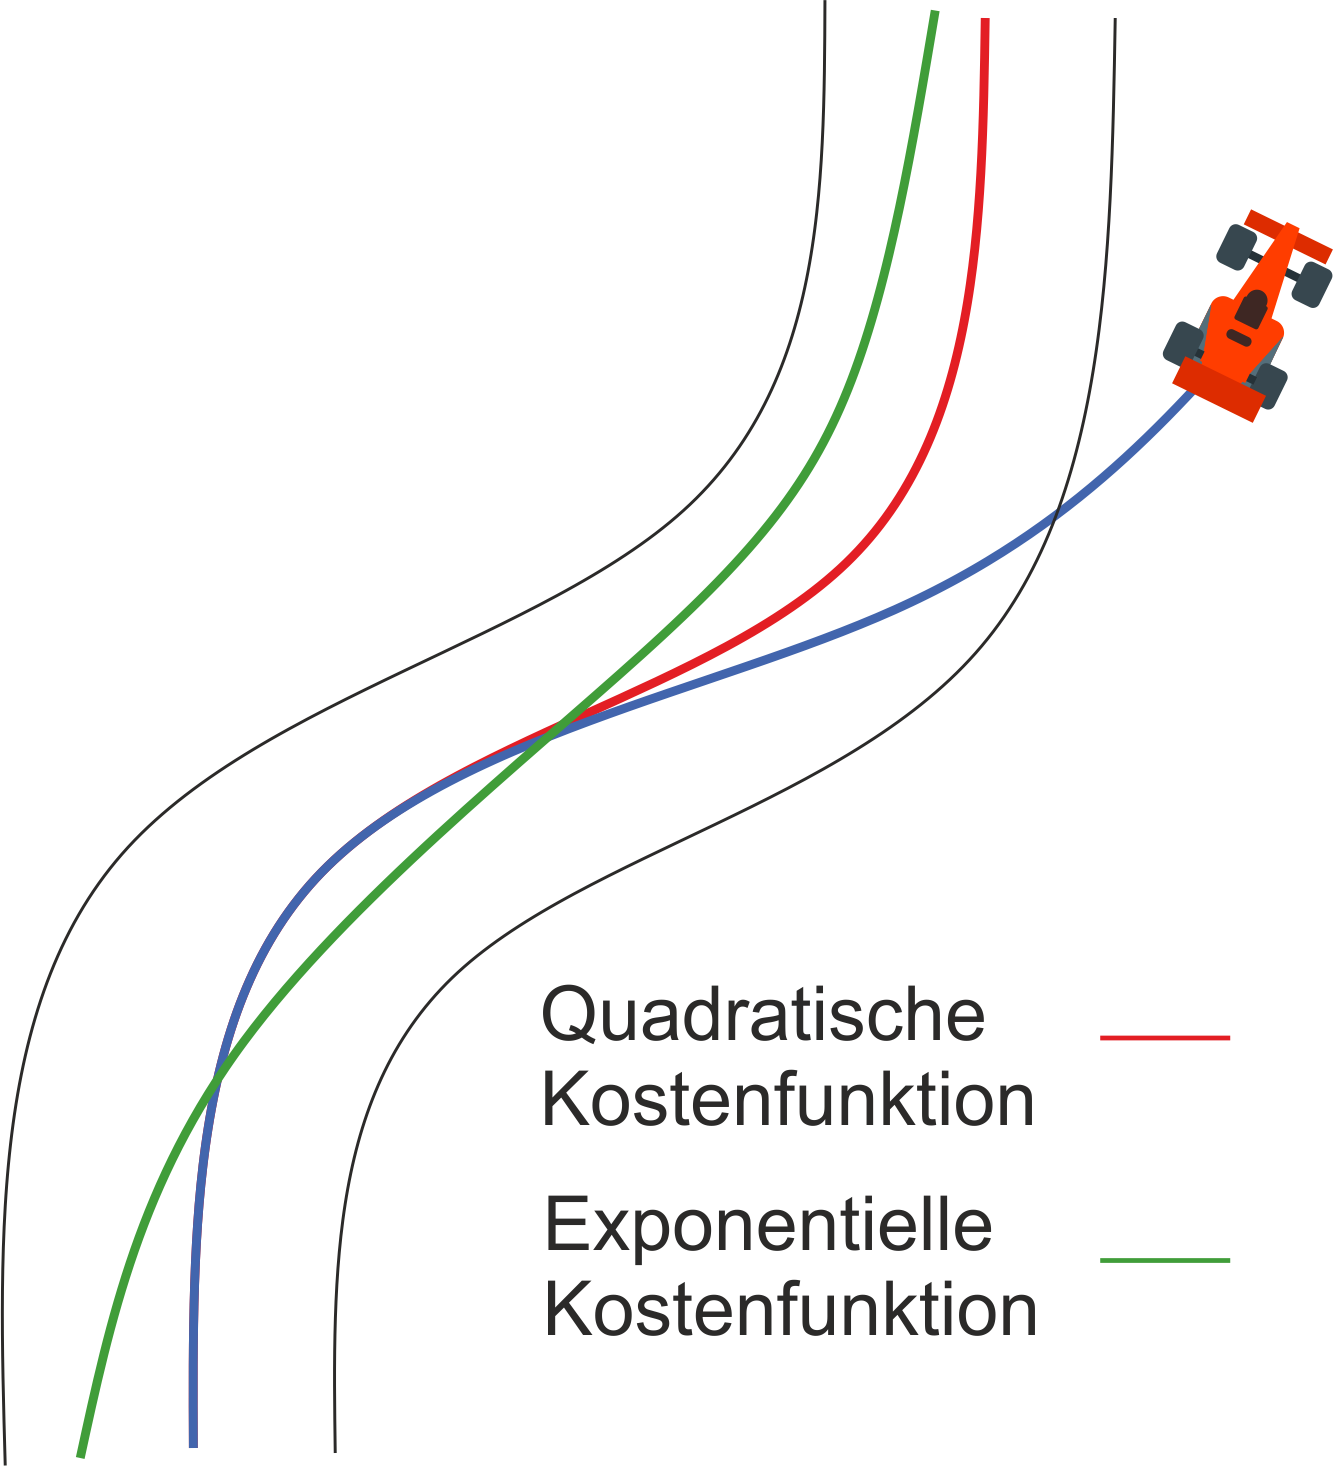
\includegraphics[width=200pt]{Abbildungen/quadraticCostFunction.png}
	\caption{Kurs auf dem sich das Fahrzeug für die quadratische Kostenfunktion bewegt}
	\label{fig:quadraticCostFunct}
\end{figure}

\chapter[Zusammenfassung]{Zusammenfassung und Ausblick}
Dieses Kapitel fasst noch einmal in kurzen Worten die Ergebnisse der Arbeit zusammen und bietet anschließend noch einige Anregungen für Verbesserungen des Algorithmus, Simulator und was in der Zukunft noch untersucht werden kann.
\section{Zusammenfassung}
In dieser Arbeit wurde eine Simulationsumgebung erstellt, die auf verschiedene Fahrzeugmodelle zurückgreifen kann und genutzt wird um die Regelbarkeit eines Rennautos mithilfe eines \ac{MPC}-Ansatzes zu überprüfen. Dies soll die Grundlage für die Entwicklung der Regelung und Trajektorienplanung des ersten High-Octane Motorsports Driverless Fahrzeug bilden. Es handelt sich dabei um ein hoch performantes Rennauto, welches für niedrige Geschwindigkeiten (bis $121$ $\frac{\text{km}}{\text{h}}$) und hohe Kurvendynamik ausgelegt ist. Besonderes Augenmerk wurde auf die Echtzeitfähigkeit und die Unterschiede zwischen den einzelnen Fahrzeugmodellen gelegt. Es ist nicht nur wichtig, ein möglichst realistisches Modell des Rennautos zu besitzen, der Algorithmus muss auch performant genug sein um eine Aktualisierungsrate von mindestens 20 Hz realisieren zu können. 
Im \ac{MPC}-Algorithmus wurde ein einfaches kinematisches Fahrzeugmodell hinterlegt um die Bewegung des Rennautos vorausberechnen zu können. Dieses wurde im Simulator durch ein deutlich realistischeres Modell, ein dynamisches Fahrzeugmodell, welches die Reifenkräfte mit betrachtet, simuliert. Die Unterschiede zwischen den Modellen wurden genutzt, um zu evaluieren wie robust der Algorithmus noch ist, wenn die hinterlegte Systembeschreibung von der Realität abweicht. Um das Fahrzeug auf der Spur zu halten ohne dass der Algorithmus bei einer Überschreitung der Seitenlinien abbricht, wurden verschiedene Kostenfunktionen untersucht, die die tangentialen Beschränkungen in die Kostenfunktion integrieren. Das beste Ergebnis lieferte eine e-Funktion, die an den Grenzen sehr schnell groß wird. Sie zeichnet sich durch eine schnelle Berechnungszeit und eine gute Approximation der tangentialen Beschränkung aus. Die Untersuchungen der Länge des Prädiktionshorizontes und der Aktualisierungsrate verdeutlichen, dass das gewählte $\Delta t$ einen größeren Einfluss auf die schnellste Rundenzeit hat als die Zeit mit der in die Zukunft prädiziert wird. Hier muss abhängig von der zur Verfügung stehenden Rechenleistung ein Kompromiss gesucht werden. Die höchste Priorität hat jedoch ein möglichst genaues Fahrzeugmodell. Durch den Umstieg im Simulator vom kinematischen auf das dynamische Fahrzeugmodell ist die Rundenzeit signifikant schlechter geworden. Mit einem genaueren Modell im \ac{MPC}-Algorithmus ist also auch mit einer besseren Regelung zu rechnen.  

\section{Ausblick}
Im nächsten Abschnitt wird kurz auf die Verbesserungsmöglichkeiten eingegangen, um den \ac{MPC}-Ansatz noch leistungsfähiger zu machen und die Simulation zu Verbessern.
\subsection{Simulator}
In der aktuellen Version des Simulators bezieht sich die Beschränkung durch die Streckenbegrenzung auf den Mittelpunkt des Fahrzeugs. Diese Einschränkung kann erweitert werden, indem die tangentialen Beschränkungen auf allen vier Rädern angewandt wird. Ein weiterer Punkt, der noch keine Beachtung gefunden hat, ist die Definition der verschiedenen Rennkurse. Die Stützpunkte mit denen der virtuelle Rennkurs definiert ist besteht aus Geraden und Punkten, die auf Kreisen mit verschiedenen Radien liegen. Im echten Straßenbau wird für den Übergang zwischen der Geraden und dem Kreis auf Klothoiden gesetzt. Das Ergebnis sind Kurven die ruckfrei bzw. ihre Krümmung eine steige Funktion der Länge sind. \\
Eine Vereinfachung, die getroffen wurde, die in der Realität eine entscheidende Rolle spielt, ist die Änderungsrate des Lenkwinkels. Im Simulator kann das Fahrzeug beliebig schnell zwischen Lenkeinschlägen wechseln. Dies ist natürlich im echten Rennauto nicht möglich. Ebenfalls vorstellbar wäre die Berücksichtigung der Bewegung des Fahrzeugs während die Regelparameter vom \ac{MPC}-Algorithmus berechnet werden. Die Stellgrößen beziehen sich auf eine Position, die nicht mehr der aktuellen entspricht, sobald die Berechnung abgeschlossen ist.

\subsection{Dynamisches Fahrzeugmodell im MPC}
In dieser Arbeit wurde untersucht, unter welchen Bedingungen ein autonomes Rennauto mit einem \ac{MPC}-Algorithmus geregelt werden kann. Das für das Fahrzeug hinterlegte Modell, welches zur Prädiktion zukünftiger Systemzustände genutzt wird, entspricht einem kinematischen Modell. Trotz dieser Einschränkung sind bereits hohe Geschwindigkeiten gut kontrollierbar. Performance an der Leistungsgrenze des Rennautos ist jedoch erst zu erwarten, wenn das dynamische Modell im \ac{MPC}-Ansatz hinterlegt wird, um die zukünftigen Zustände zu berechnen. An diesem Punkt würden der Regler auch die ganze Querdynamik des Fahrzeugs mit in die Lösung einbeziehen. Es muss untersucht werden, welche Einschränkungen das für die Länge des prädizierten Horizontes bedeutet, da die Komplexität der Berechnung steigt. Die Messungen in Kapitel \ref{laptime} haben jedoch ergeben, dass der größere Prädiktionshorizont weniger Einfluss auf die Rundenzeit als das Modell hat.

\subsection{Zweispurmodell}
Im High-Octane Motorsports Verein ist eine Rundenzeitsimulation in der Entwicklung. Für diese wird ein genaues Zweispurmodell genutzt, welches das Fahrwerk, Abtrieb, Nicken, Rollen, Federkräfte und ein sehr genaues Reifenmodell berücksichtigt. Die Berechnungszeit ist nicht mehr in einem Bereich, der in Echtzeit realisierbar ist. Für die Steuerparameter könnte das Modell trotzdem mit dem \ac{MPC}-Ansatz kombiniert werden, um die idealen Steuerparameter zu finden, um die Rundenzeitsimulation zu realisieren. 

\subsection{Implementierung in C++}
Im Driverless-Projekt des High-Octane Vereins wird die Middleware \ac{ROS} verwendet um die Software des autonomen Rennautos zu entwickeln. \ac{ROS} unterstützt nativ nur Python und C++. Daher sollte der Algorithmus in C++ implementiert werden, um eine möglichst hohe Performance zu gewährleisten. 
Es gibt noch kein Framework wie \ac{Jump} für C++, welches die Verwendung des Optimierers und die automatische Ableitung kombiniert. Diese zwei Bestandteile müssen also manuell integriert werden. Für die automatische Ableitung kann zum Beispiel das CppAd Paket verwendet werden, welches unter der Common Public License veröffentlicht wird. Der Optimierer \ac{Ipopt} ist in C++ implementiert und daher direkt integrierbar. 
Ein anderer Weg wäre es den \ac{MPC}-Ansatz in Python mit dem \ac{Jump} ähnlichen Framework CasADi zu implementiere. Wie der Benchmark \ref{fig:juliaBench} in Kapitel \ref{julia} jedoch gezeigt hat ist eine höhere Performance von einer C-Nahen Implementierung zu erwarten. 

\subsection{Fahrzeugparameter anpassen}
Wie bereits im Stand der Technik ausgeführt, kann nichtlineare Regression dazu verwendet werden die Werte, mit denen das Modell parametrisiert ist zu verbessern. Das Rennauto wird von einem menschlichen Fahrer in verschiedenen Szenarien gefahren werden und sowohl die Steuerparameter (Gas, Bremse, Lenkung) wie auch der Fahrzeugzustand mit möglichst hoher Frequenz abgespeichert. Die so erfassten Daten werden genutzt um die Parameter des Modells anzupassen und die Differenz zwischen Modell und Realität zu minimieren. 


\appendix

%\chapter*{Anhang}
%\large{
%Anhang 1\par
%Anhang 2


% setzt die Bildunterschriften auf A1 (A=Anhang)
\renewcommand{\thefigure}{A\arabic{figure}} 
\chapter{Anhang}

\subsection*{Elektronischer Anhang }

\subsection*{Fahrzeugdaten}
\begin{figure}[hb!]
	\caption{Engine Power}
	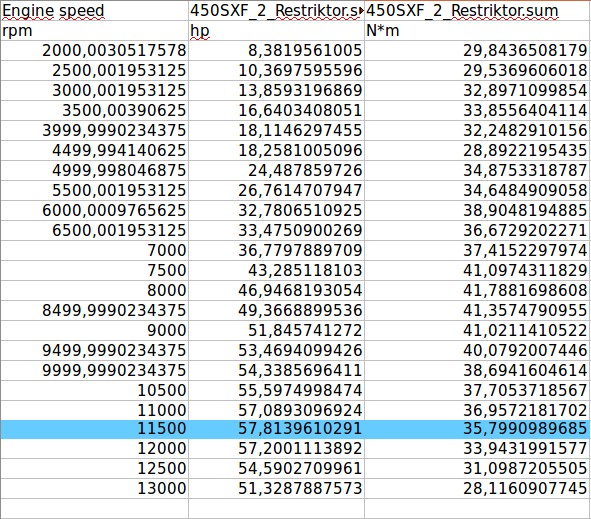
\includegraphics[width=350pt]{Abbildungen/Engine_power.png}
	\label{fig:enginePower}
\end{figure}

\begin{figure}[hb!]
	\caption{Max Tire Force}
	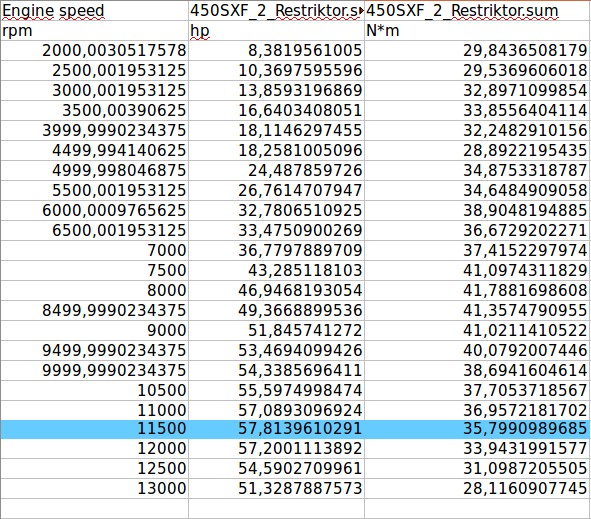
\includegraphics[width=350pt]{Abbildungen/Engine_power.png}
	\label{fig:maxTireForce}
\end{figure}



 \subsection*{Einbindung Grafik im Anhang}
  \begin{figure}[h!]
  \begin{centering}
  {
\includegraphics[width=0.33\textwidth]{Abbildungen/fau.png}}
   \caption{Unterschrift Bild x Die auf die Rotationsfrequenz des Innenzylinders normierten Eigenfrequenzen der gefun-denen Grundmoden der Taylor-Strömung für h(Die azimutale Wellenzahl ist mit m  bezeichnet.)}
  \end{centering}
  \end{figure}

\subsection{Code}

\begin{lstlisting}
[caption={ein paar Zeilen code}\label{lst:vehicleModel},captionpos=t] 
    for i in 0: N-1
    
    @NLexpression(m, x_dd, (VehicleModel.max_long_acc * x[8*i + 7]/10.0))
    
    @NLconstraints(m, begin
    x[(i + 1)*8 + 1] - (x[i * 8 + 1] + x[8*i + 3]*
    dt*cos(x[i*8 + 4] + atan(lr/(lf + lr) * tan(x[i*8 + 8])))) == 0
    x[(i + 1)*8 + 2] - (x[i * 8 + 2] + x[8*i + 3]*
    dt*sin(x[i*8 + 4] + atan(lr/(lf + lr) * tan(x[i*8 + 8])))) == 0
    x[(i + 1)*8 + 3] - (x[i * 8 + 3] + x_dd*dt) == 0
    x[(i + 1)*8 + 4] - (x[i * 8 + 4] + x[8*i + 3]*
    dt / lr*sin(atan(lr/(lf + lr) * tan(x[i*8 + 8])))) == 0
    atan(0.5 * (lf + lr) * mpc_struct.beta_max / x[i*8 + 3]^2)
    - atan(lr/(lf + lf) * tan(x[i*8 + 8])) >= 0  #max_beta - beta
    atan(0.5 * (lf + lr) * mpc_struct.beta_max / x[i*8 + 3]^2)
    + atan(lr/(lf + lf) * tan(x[i*8 + 8])) >= 0  #max_beta + beta
    end)
    end
\end{lstlisting}







%Abkürzungsverzeichnis
%\pagestyle{scrheadings}
%\chapter*{Abkürzungsverzeichnis}

\chapter*{Abkürzungsverzeichnis}
\addcontentsline{toc}{chapter}{Abkürzungsverzeichnis} %Abkürzungsverzeichnis kommt ins InhaV.





\begin{acronym}[SEPSEP] 
 \acro{Abk.}{Abkürzung}
 \acro{z.B.}{zum Beispiel}
 \acro{MPC}{Model Predictive Control}
 \acro{JIT}{just-in-time}
 \acro{SLSQP}{Sequential Least SQuarez Programming}
\end{acronym}




%\bibliographystyle{IEEEtran}
\bibliographystyle{alpha}
\bibliography{Inhalt/literatur}
\listoffigures
\listoftables

% Bitte noch Index anhängen (kommt unter Linux zu Fehlermeldungen)
%





%\printindex


%bitte Lebenslauf anhängen !!!
% kommt unter Linux zu Fehlermeldungen

%%%%%%%%%%%%%%%%%%%%%%%%%%%%%%%%%%%%%%%%%%%%%%%%%%%%%
          %   \begin  CV und Beginn des Dokuments
%%%%%%%%%%%%%%%%%%%%%%%%%%%%%%%%%%%%%%%%%%%%%%%%%%%%
%\enlargethispage{3cm}

\chapter*{Albert Einstein}
\markboth{Albert Einstein}{Albert Einstein} % falls der CV über 2 Seiten geht um einen "Running Header" zu haben


\flushright
% Code mit Bild:
%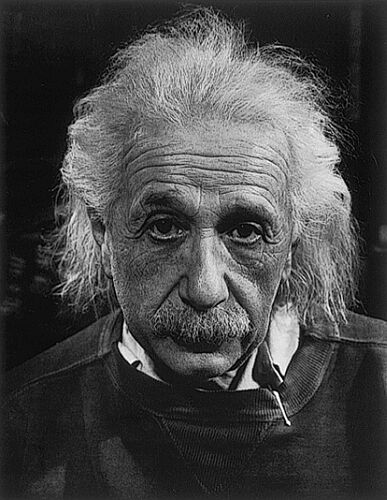
\includegraphics[scale=.2]{Abbildungen/albert-einstein.jpg}
%\vspace*{-5cm}{
%Code ohne Bild:
%\vspace*{-1cm}{
\subsection*{Persönliche Daten}
\flushleft
%\tabular-Umgebung
\normalsize
\begin{tabular}{lcl}
Adresse             & ~ & Albert-Einstein-Straße 98\\
                    & ~ & 91058 Erlangen\\[5pt]
Mobil               & ~ & 0151 - 12345978\\
Email               & ~ & albert@einstein.de\\[5pt]
Geburtsdatum        & ~ & 10.10.1910\\
Staatsangehörigkeit & ~ & deutsch\\
\end{tabular} 

\subsection*{Bachelorarbeit (optionaler Punkt)}
\begin{tabular}{lcl}
01/2016-07/2016     & ~~~~~ & Bachelorarbeit \\
                    & ~~~~~ & Ich bin das Thema der Bachelorarbeit\\[5pt]

\end{tabular} 
\\*  % Zeilenumbruch OHNE Seitenwechsel

\nopagebreak
\subsection*{Studium und Schulbildung}
\begin{tabular}{lcl}
01/2016 - 07/2016     & ~~~ &  Friedrich-Alexander-Universität Erlangen-Nürnberg\\
                      & ~~~ &  Hauptfächer Prokrastination und Bummelei\\
01/2010 - 01/2016     & ~~~ &  Albert-Einstein-Gymnasium, Erlangen\\
                      & ~~~ &  Leistungskurse: Feiern und Relaxen\\
\end{tabular}

\subsection*{Berufliche Erfahrungen / Praktika}
\begin{tabular}{lcl}
01/2016 - 07/2016     & ~~~ &  Wissenschaftlicher Hilfsmitarbeiter am Fraunhofer IIS\\
01/2016 - 07/2016     & ~~~ &  Praktikum bei Siemens Erlangen\\
\end{tabular}
\subsection*{Zusatzqualifikationen - (optional)}
\begin{tabular}{lcl}
Sprachen            &  & Deutsch (Muttersprache)\\
                    &  & Englisch (fließend in Wort und Schrift)\\
                    &  & Französisch (Grundkenntnisse)\\[5pt]
Programmiersprachen &  & Java \\
\end{tabular} 
\bigskip
\vspace*{.5cm}




Erlangen, den (Datum eintragen)\\*[20pt]\nopagebreak
\vspace{0.5cm}


\rule{5cm}{0.4pt}\\*\nopagebreak


Albert Einstein\\*\nopagebreak







\end{document}



 
